\documentclass[man,floatsintext]{apa7}

\usepackage{rotating}
\usepackage{graphicx}
\usepackage{caption}
\usepackage{hyperref}
\usepackage{enumitem}
\usepackage{subcaption}
\usepackage{pdfpages}
\usepackage{amsmath}
\usepackage{longtable}
\usepackage{soul}
\usepackage{arydshln}
\usepackage{threeparttable}
% keep every table and figure within its own section (no drifting to the end)
\usepackage[section]{placeins}

\usepackage{listings}
\usepackage{xcolor}


\usepackage{soul}
\usepackage[utf8]{inputenc}
\usepackage[export]{adjustbox}
\usepackage[style=apa,sortcites=true,sorting=nyt,backend=biber]{biblatex}

\DeclareFieldFormat{apacase}{#1}

\addbibresource{lit.bib}

% synthetic-data version: the revision markup is printed as plain text, so
% that only purple (synthetic results) and red (text that does not fit them)
% carry meaning
\newcommand{\change}[1]{#1}

% All numbers from the analysis: \res{<key>}, written by run_all.R
% (keys and values are listed in generated/results.tex)
% generated by R/export_tex.R -- do not edit by hand.
% run: 2026-11-19 00:00
%
% \res{<key>} prints a value; an unknown key prints a red ??<key>.
\newcommand{\res}[1]{\ifcsname res@#1\endcsname\csname res@#1\endcsname\else\textbf{\textcolor{red}{??\detokenize{#1}}}\fi}
\newcommand{\resrundate}{2026-11-19}
% SYNTHETIC data: every value below is wrapped in \synth (purple);
% \synthmismatch marks manuscript sentences that do not fit the synthetic results (red).
\providecommand{\synth}[1]{\textcolor[HTML]{7B1FA2}{#1}}
\providecommand{\synthmismatch}[1]{\textcolor{red}{#1}}

\expandafter\def\csname res@apeq.cor.who.aaq\endcsname{\synth{\ensuremath{-}.686}}
\expandafter\def\csname res@bge.apeq.aaq.best.cihi\endcsname{\synth{.055}}
\expandafter\def\csname res@bge.apeq.aaq.best.cilo\endcsname{\synth{.018}}
\expandafter\def\csname res@bge.apeq.aaq.best.delta\endcsname{\synth{.037}}
\expandafter\def\csname res@bge.apeq.aaq.best.deltapct\endcsname{\synth{3.7}}
\expandafter\def\csname res@bge.apeq.aaq.best.df\endcsname{\synth{99}}
\expandafter\def\csname res@bge.apeq.aaq.best.model\endcsname{\synth{text}}
\expandafter\def\csname res@bge.apeq.aaq.best.p\endcsname{\synth{\ensuremath{p < .001}}}
\expandafter\def\csname res@bge.apeq.aaq.best.r2\endcsname{\synth{.436}}
\expandafter\def\csname res@bge.apeq.aaq.best.relgain\endcsname{\synth{9.2}}
\expandafter\def\csname res@bge.apeq.aaq.best.t\endcsname{\synth{3.91}}
\expandafter\def\csname res@bge.apeq.aaq.confirm.cihi\endcsname{\synth{.055}}
\expandafter\def\csname res@bge.apeq.aaq.confirm.cilo\endcsname{\synth{.018}}
\expandafter\def\csname res@bge.apeq.aaq.confirm.delta\endcsname{\synth{.037}}
\expandafter\def\csname res@bge.apeq.aaq.confirm.deltapct\endcsname{\synth{3.7}}
\expandafter\def\csname res@bge.apeq.aaq.confirm.df\endcsname{\synth{99}}
\expandafter\def\csname res@bge.apeq.aaq.confirm.model\endcsname{\synth{text}}
\expandafter\def\csname res@bge.apeq.aaq.confirm.p\endcsname{\synth{\ensuremath{p < .001}}}
\expandafter\def\csname res@bge.apeq.aaq.confirm.r2\endcsname{\synth{.436}}
\expandafter\def\csname res@bge.apeq.aaq.confirm.relgain\endcsname{\synth{9.2}}
\expandafter\def\csname res@bge.apeq.aaq.confirm.t\endcsname{\synth{3.91}}
\expandafter\def\csname res@bge.apeq.aaq.examples.model\endcsname{\synth{text}}
\expandafter\def\csname res@bge.apeq.aaq.examples.ndropped\endcsname{\synth{0}}
\expandafter\def\csname res@bge.apeq.aaq.none.alpha\endcsname{\synth{0.1}}
\expandafter\def\csname res@bge.apeq.aaq.none.lambda\endcsname{\synth{1.23}}
\expandafter\def\csname res@bge.apeq.aaq.none.nna\endcsname{\synth{0}}
\expandafter\def\csname res@bge.apeq.aaq.none.r2\endcsname{\synth{.399}}
\expandafter\def\csname res@bge.apeq.aaq.none.single.alpha\endcsname{\synth{0.1}}
\expandafter\def\csname res@bge.apeq.aaq.none.single.lambda\endcsname{\synth{0.977}}
\expandafter\def\csname res@bge.apeq.aaq.none.single.r2\endcsname{\synth{.408}}
\expandafter\def\csname res@bge.apeq.aaq.singlebest.delta\endcsname{\synth{.038}}
\expandafter\def\csname res@bge.apeq.aaq.singlebest.deltapct\endcsname{\synth{3.8}}
\expandafter\def\csname res@bge.apeq.aaq.singlebest.model\endcsname{\synth{text}}
\expandafter\def\csname res@bge.apeq.aaq.singlebest.r2\endcsname{\synth{.446}}
\expandafter\def\csname res@bge.apeq.aaq.singlebest.relgain\endcsname{\synth{9.3}}
\expandafter\def\csname res@bge.apeq.aaq.sweepbest.delta\endcsname{\synth{.038}}
\expandafter\def\csname res@bge.apeq.aaq.sweepbest.model\endcsname{\synth{text}}
\expandafter\def\csname res@bge.apeq.aaq.sweepbest.nprin\endcsname{\synth{18}}
\expandafter\def\csname res@bge.apeq.aaq.sweepbest.r2\endcsname{\synth{.446}}
\expandafter\def\csname res@bge.apeq.aaq.text.alpha\endcsname{\synth{0.0}}
\expandafter\def\csname res@bge.apeq.aaq.text.cihi\endcsname{\synth{.055}}
\expandafter\def\csname res@bge.apeq.aaq.text.cilo\endcsname{\synth{.018}}
\expandafter\def\csname res@bge.apeq.aaq.text.delta\endcsname{\synth{.037}}
\expandafter\def\csname res@bge.apeq.aaq.text.deltapct\endcsname{\synth{3.7}}
\expandafter\def\csname res@bge.apeq.aaq.text.df\endcsname{\synth{99}}
\expandafter\def\csname res@bge.apeq.aaq.text.lambda\endcsname{\synth{4.98}}
\expandafter\def\csname res@bge.apeq.aaq.text.mcse\endcsname{\synth{0.0014}}
\expandafter\def\csname res@bge.apeq.aaq.text.nna\endcsname{\synth{0}}
\expandafter\def\csname res@bge.apeq.aaq.text.p\endcsname{\synth{\ensuremath{p < .001}}}
\expandafter\def\csname res@bge.apeq.aaq.text.r2\endcsname{\synth{.436}}
\expandafter\def\csname res@bge.apeq.aaq.text.relgain\endcsname{\synth{9.2}}
\expandafter\def\csname res@bge.apeq.aaq.text.single.alpha\endcsname{\synth{0.0}}
\expandafter\def\csname res@bge.apeq.aaq.text.single.delta\endcsname{\synth{.038}}
\expandafter\def\csname res@bge.apeq.aaq.text.single.deltapct\endcsname{\synth{3.8}}
\expandafter\def\csname res@bge.apeq.aaq.text.single.lambda\endcsname{\synth{3.51}}
\expandafter\def\csname res@bge.apeq.aaq.text.single.r2\endcsname{\synth{.446}}
\expandafter\def\csname res@bge.apeq.aaq.text.single.relgain\endcsname{\synth{9.3}}
\expandafter\def\csname res@bge.apeq.aaq.text.sweepbest.delta\endcsname{\synth{.038}}
\expandafter\def\csname res@bge.apeq.aaq.text.sweepbest.nprin\endcsname{\synth{18}}
\expandafter\def\csname res@bge.apeq.aaq.text.sweepbest.r2\endcsname{\synth{.446}}
\expandafter\def\csname res@bge.apeq.aaq.text.t\endcsname{\synth{3.91}}
\expandafter\def\csname res@bge.apeq.aaq.textonly.alpha\endcsname{\synth{0.1}}
\expandafter\def\csname res@bge.apeq.aaq.textonly.lambda\endcsname{\synth{0.486}}
\expandafter\def\csname res@bge.apeq.aaq.textonly.nna\endcsname{\synth{0}}
\expandafter\def\csname res@bge.apeq.aaq.textonly.r2\endcsname{\synth{.197}}
\expandafter\def\csname res@bge.apeq.aaq.textonly.single.alpha\endcsname{\synth{0.0}}
\expandafter\def\csname res@bge.apeq.aaq.textonly.single.delta\endcsname{\synth{\ensuremath{-}.194}}
\expandafter\def\csname res@bge.apeq.aaq.textonly.single.deltapct\endcsname{\synth{\ensuremath{-}19.4}}
\expandafter\def\csname res@bge.apeq.aaq.textonly.single.lambda\endcsname{\synth{7.92}}
\expandafter\def\csname res@bge.apeq.aaq.textonly.single.r2\endcsname{\synth{.214}}
\expandafter\def\csname res@bge.apeq.aaq.textonly.single.relgain\endcsname{\synth{\ensuremath{-}47.5}}
\expandafter\def\csname res@bge.apeq.aaq.textonly.sweepbest.delta\endcsname{\synth{\ensuremath{-}.194}}
\expandafter\def\csname res@bge.apeq.aaq.textonly.sweepbest.nprin\endcsname{\synth{20}}
\expandafter\def\csname res@bge.apeq.aaq.textonly.sweepbest.r2\endcsname{\synth{.214}}
\expandafter\def\csname res@bge.apeq.aaq.textsignal.r2\endcsname{\synth{.290}}
\expandafter\def\csname res@bge.apeq.overlap.age...jahre\endcsname{\synth{.011}}
\expandafter\def\csname res@bge.apeq.overlap.apeq-acpe\endcsname{\synth{.219}}
\expandafter\def\csname res@bge.apeq.overlap.apeq-avpe\endcsname{\synth{.002}}
\expandafter\def\csname res@bge.apeq.overlap.ceq-total\endcsname{\synth{.060}}
\expandafter\def\csname res@bge.apeq.overlap.dose\endcsname{\synth{.018}}
\expandafter\def\csname res@bge.apeq.overlap.duration\endcsname{\synth{\ensuremath{-}.001}}
\expandafter\def\csname res@bge.apeq.overlap.ebi-total\endcsname{\synth{.101}}
\expandafter\def\csname res@bge.apeq.overlap.factor1-therapeutic\endcsname{\synth{.180}}
\expandafter\def\csname res@bge.apeq.overlap.factor2-escapist\endcsname{\synth{\ensuremath{-}.011}}
\expandafter\def\csname res@bge.apeq.overlap.factor3-hedonic\endcsname{\synth{\ensuremath{-}.001}}
\expandafter\def\csname res@bge.apeq.overlap.group\endcsname{\synth{text}}
\expandafter\def\csname res@bge.apeq.overlap.mood\endcsname{\synth{\ensuremath{-}.002}}
\expandafter\def\csname res@bge.apeq.overlap.n\endcsname{\synth{958}}
\expandafter\def\csname res@bge.apeq.overlap.nbinary\endcsname{\synth{0}}
\expandafter\def\csname res@bge.apeq.overlap.nmultilevel\endcsname{\synth{3}}
\expandafter\def\csname res@bge.apeq.overlap.nrare\endcsname{\synth{0}}
\expandafter\def\csname res@bge.apeq.overlap.preparedness\endcsname{\synth{.009}}
\expandafter\def\csname res@bge.apeq.overlap.retrospectiveappraisal\endcsname{\synth{.121}}
\expandafter\def\csname res@bge.apeq.overlap.strength\endcsname{\synth{\ensuremath{-}.001}}
\expandafter\def\csname res@bge.apeq.overlap.valence\endcsname{\synth{.001}}
\expandafter\def\csname res@bge.apeq.who.best.cihi\endcsname{\synth{.074}}
\expandafter\def\csname res@bge.apeq.who.best.cilo\endcsname{\synth{.029}}
\expandafter\def\csname res@bge.apeq.who.best.delta\endcsname{\synth{.051}}
\expandafter\def\csname res@bge.apeq.who.best.deltapct\endcsname{\synth{5.1}}
\expandafter\def\csname res@bge.apeq.who.best.df\endcsname{\synth{99}}
\expandafter\def\csname res@bge.apeq.who.best.model\endcsname{\synth{text}}
\expandafter\def\csname res@bge.apeq.who.best.p\endcsname{\synth{\ensuremath{p < .001}}}
\expandafter\def\csname res@bge.apeq.who.best.r2\endcsname{\synth{.421}}
\expandafter\def\csname res@bge.apeq.who.best.relgain\endcsname{\synth{13.9}}
\expandafter\def\csname res@bge.apeq.who.best.t\endcsname{\synth{4.56}}
\expandafter\def\csname res@bge.apeq.who.confirm.cihi\endcsname{\synth{.074}}
\expandafter\def\csname res@bge.apeq.who.confirm.cilo\endcsname{\synth{.029}}
\expandafter\def\csname res@bge.apeq.who.confirm.delta\endcsname{\synth{.051}}
\expandafter\def\csname res@bge.apeq.who.confirm.deltapct\endcsname{\synth{5.1}}
\expandafter\def\csname res@bge.apeq.who.confirm.df\endcsname{\synth{99}}
\expandafter\def\csname res@bge.apeq.who.confirm.model\endcsname{\synth{text}}
\expandafter\def\csname res@bge.apeq.who.confirm.p\endcsname{\synth{\ensuremath{p < .001}}}
\expandafter\def\csname res@bge.apeq.who.confirm.r2\endcsname{\synth{.421}}
\expandafter\def\csname res@bge.apeq.who.confirm.relgain\endcsname{\synth{13.9}}
\expandafter\def\csname res@bge.apeq.who.confirm.t\endcsname{\synth{4.56}}
\expandafter\def\csname res@bge.apeq.who.examples.model\endcsname{\synth{text}}
\expandafter\def\csname res@bge.apeq.who.examples.ndropped\endcsname{\synth{0}}
\expandafter\def\csname res@bge.apeq.who.none.alpha\endcsname{\synth{0.2}}
\expandafter\def\csname res@bge.apeq.who.none.lambda\endcsname{\synth{0.114}}
\expandafter\def\csname res@bge.apeq.who.none.nna\endcsname{\synth{0}}
\expandafter\def\csname res@bge.apeq.who.none.r2\endcsname{\synth{.369}}
\expandafter\def\csname res@bge.apeq.who.none.single.alpha\endcsname{\synth{0.1}}
\expandafter\def\csname res@bge.apeq.who.none.single.lambda\endcsname{\synth{0.774}}
\expandafter\def\csname res@bge.apeq.who.none.single.r2\endcsname{\synth{.373}}
\expandafter\def\csname res@bge.apeq.who.singlebest.delta\endcsname{\synth{.049}}
\expandafter\def\csname res@bge.apeq.who.singlebest.deltapct\endcsname{\synth{4.9}}
\expandafter\def\csname res@bge.apeq.who.singlebest.model\endcsname{\synth{text}}
\expandafter\def\csname res@bge.apeq.who.singlebest.r2\endcsname{\synth{.422}}
\expandafter\def\csname res@bge.apeq.who.singlebest.relgain\endcsname{\synth{13.2}}
\expandafter\def\csname res@bge.apeq.who.sweepbest.delta\endcsname{\synth{.049}}
\expandafter\def\csname res@bge.apeq.who.sweepbest.model\endcsname{\synth{text}}
\expandafter\def\csname res@bge.apeq.who.sweepbest.nprin\endcsname{\synth{30}}
\expandafter\def\csname res@bge.apeq.who.sweepbest.r2\endcsname{\synth{.422}}
\expandafter\def\csname res@bge.apeq.who.text.alpha\endcsname{\synth{0.2}}
\expandafter\def\csname res@bge.apeq.who.text.cihi\endcsname{\synth{.074}}
\expandafter\def\csname res@bge.apeq.who.text.cilo\endcsname{\synth{.029}}
\expandafter\def\csname res@bge.apeq.who.text.delta\endcsname{\synth{.051}}
\expandafter\def\csname res@bge.apeq.who.text.deltapct\endcsname{\synth{5.1}}
\expandafter\def\csname res@bge.apeq.who.text.df\endcsname{\synth{99}}
\expandafter\def\csname res@bge.apeq.who.text.lambda\endcsname{\synth{0.689}}
\expandafter\def\csname res@bge.apeq.who.text.mcse\endcsname{\synth{0.00084}}
\expandafter\def\csname res@bge.apeq.who.text.nna\endcsname{\synth{0}}
\expandafter\def\csname res@bge.apeq.who.text.p\endcsname{\synth{\ensuremath{p < .001}}}
\expandafter\def\csname res@bge.apeq.who.text.r2\endcsname{\synth{.421}}
\expandafter\def\csname res@bge.apeq.who.text.relgain\endcsname{\synth{13.9}}
\expandafter\def\csname res@bge.apeq.who.text.single.alpha\endcsname{\synth{0.1}}
\expandafter\def\csname res@bge.apeq.who.text.single.delta\endcsname{\synth{.049}}
\expandafter\def\csname res@bge.apeq.who.text.single.deltapct\endcsname{\synth{4.9}}
\expandafter\def\csname res@bge.apeq.who.text.single.lambda\endcsname{\synth{0.87}}
\expandafter\def\csname res@bge.apeq.who.text.single.r2\endcsname{\synth{.422}}
\expandafter\def\csname res@bge.apeq.who.text.single.relgain\endcsname{\synth{13.2}}
\expandafter\def\csname res@bge.apeq.who.text.sweepbest.delta\endcsname{\synth{.049}}
\expandafter\def\csname res@bge.apeq.who.text.sweepbest.nprin\endcsname{\synth{30}}
\expandafter\def\csname res@bge.apeq.who.text.sweepbest.r2\endcsname{\synth{.422}}
\expandafter\def\csname res@bge.apeq.who.text.t\endcsname{\synth{4.56}}
\expandafter\def\csname res@bge.apeq.who.textonly.alpha\endcsname{\synth{0.3}}
\expandafter\def\csname res@bge.apeq.who.textonly.lambda\endcsname{\synth{0.135}}
\expandafter\def\csname res@bge.apeq.who.textonly.nna\endcsname{\synth{0}}
\expandafter\def\csname res@bge.apeq.who.textonly.r2\endcsname{\synth{.224}}
\expandafter\def\csname res@bge.apeq.who.textonly.single.alpha\endcsname{\synth{0.1}}
\expandafter\def\csname res@bge.apeq.who.textonly.single.delta\endcsname{\synth{\ensuremath{-}.144}}
\expandafter\def\csname res@bge.apeq.who.textonly.single.deltapct\endcsname{\synth{\ensuremath{-}14.4}}
\expandafter\def\csname res@bge.apeq.who.textonly.single.lambda\endcsname{\synth{0.774}}
\expandafter\def\csname res@bge.apeq.who.textonly.single.r2\endcsname{\synth{.229}}
\expandafter\def\csname res@bge.apeq.who.textonly.single.relgain\endcsname{\synth{\ensuremath{-}38.5}}
\expandafter\def\csname res@bge.apeq.who.textonly.sweepbest.delta\endcsname{\synth{\ensuremath{-}.140}}
\expandafter\def\csname res@bge.apeq.who.textonly.sweepbest.nprin\endcsname{\synth{22}}
\expandafter\def\csname res@bge.apeq.who.textonly.sweepbest.r2\endcsname{\synth{.232}}
\expandafter\def\csname res@bge.apeq.who.textsignal.r2\endcsname{\synth{.319}}
\expandafter\def\csname res@bge.gcmq.overlap.age\endcsname{\synth{.014}}
\expandafter\def\csname res@bge.gcmq.overlap.apeq-ace\endcsname{\synth{\ensuremath{-}.006}}
\expandafter\def\csname res@bge.gcmq.overlap.apeq-ave\endcsname{\synth{.013}}
\expandafter\def\csname res@bge.gcmq.overlap.asc-obe\endcsname{\synth{.095}}
\expandafter\def\csname res@bge.gcmq.overlap.ceq\endcsname{\synth{.032}}
\expandafter\def\csname res@bge.gcmq.overlap.clarity\endcsname{\synth{\ensuremath{-}.001}}
\expandafter\def\csname res@bge.gcmq.overlap.conc-none\endcsname{\synth{.041}}
\expandafter\def\csname res@bge.gcmq.overlap.cumsle\endcsname{\synth{.033}}
\expandafter\def\csname res@bge.gcmq.overlap.depression\endcsname{\synth{.038}}
\expandafter\def\csname res@bge.gcmq.overlap.diagnosis\endcsname{\synth{.055}}
\expandafter\def\csname res@bge.gcmq.overlap.dose\endcsname{\synth{\ensuremath{-}.014}}
\expandafter\def\csname res@bge.gcmq.overlap.ebi\endcsname{\synth{.000}}
\expandafter\def\csname res@bge.gcmq.overlap.gcmq-cl\endcsname{\synth{.036}}
\expandafter\def\csname res@bge.gcmq.overlap.gcmq-ma\endcsname{\synth{.002}}
\expandafter\def\csname res@bge.gcmq.overlap.gcmq-pa\endcsname{\synth{\ensuremath{-}.009}}
\expandafter\def\csname res@bge.gcmq.overlap.gcmq-ra\endcsname{\synth{.098}}
\expandafter\def\csname res@bge.gcmq.overlap.group\endcsname{\synth{health}}
\expandafter\def\csname res@bge.gcmq.overlap.int-esca\endcsname{\synth{.120}}
\expandafter\def\csname res@bge.gcmq.overlap.int-hedo\endcsname{\synth{\ensuremath{-}.004}}
\expandafter\def\csname res@bge.gcmq.overlap.int-ther\endcsname{\synth{.089}}
\expandafter\def\csname res@bge.gcmq.overlap.n\endcsname{\synth{605}}
\expandafter\def\csname res@bge.gcmq.overlap.nbinary\endcsname{\synth{4}}
\expandafter\def\csname res@bge.gcmq.overlap.nmultilevel\endcsname{\synth{3}}
\expandafter\def\csname res@bge.gcmq.overlap.nrare\endcsname{\synth{18}}
\expandafter\def\csname res@bge.gcmq.overlap.retrospectiveappraisal\endcsname{\synth{.032}}
\expandafter\def\csname res@bge.gcmq.overlap.settingnature\endcsname{\synth{.037}}
\expandafter\def\csname res@bge.gcmq.overlap.suitability\endcsname{\synth{.017}}
\expandafter\def\csname res@bge.gcmq.overlap.valence\endcsname{\synth{.022}}
\expandafter\def\csname res@bge.gcmq.wemwbs.best.cihi\endcsname{\synth{.015}}
\expandafter\def\csname res@bge.gcmq.wemwbs.best.cilo\endcsname{\synth{\ensuremath{-}.010}}
\expandafter\def\csname res@bge.gcmq.wemwbs.best.delta\endcsname{\synth{.002}}
\expandafter\def\csname res@bge.gcmq.wemwbs.best.deltapct\endcsname{\synth{0.2}}
\expandafter\def\csname res@bge.gcmq.wemwbs.best.df\endcsname{\synth{99}}
\expandafter\def\csname res@bge.gcmq.wemwbs.best.model\endcsname{\synth{health}}
\expandafter\def\csname res@bge.gcmq.wemwbs.best.p\endcsname{\synth{\ensuremath{p = .689}}}
\expandafter\def\csname res@bge.gcmq.wemwbs.best.r2\endcsname{\synth{.210}}
\expandafter\def\csname res@bge.gcmq.wemwbs.best.relgain\endcsname{\synth{1.2}}
\expandafter\def\csname res@bge.gcmq.wemwbs.best.t\endcsname{\synth{0.40}}
\expandafter\def\csname res@bge.gcmq.wemwbs.confirm.cihi\endcsname{\synth{.014}}
\expandafter\def\csname res@bge.gcmq.wemwbs.confirm.cilo\endcsname{\synth{\ensuremath{-}.015}}
\expandafter\def\csname res@bge.gcmq.wemwbs.confirm.delta\endcsname{\synth{.000}}
\expandafter\def\csname res@bge.gcmq.wemwbs.confirm.deltapct\endcsname{\synth{\ensuremath{-}0.0}}
\expandafter\def\csname res@bge.gcmq.wemwbs.confirm.df\endcsname{\synth{99}}
\expandafter\def\csname res@bge.gcmq.wemwbs.confirm.model\endcsname{\synth{events + health}}
\expandafter\def\csname res@bge.gcmq.wemwbs.confirm.p\endcsname{\synth{\ensuremath{p = .975}}}
\expandafter\def\csname res@bge.gcmq.wemwbs.confirm.r2\endcsname{\synth{.207}}
\expandafter\def\csname res@bge.gcmq.wemwbs.confirm.relgain\endcsname{\synth{\ensuremath{-}0.1}}
\expandafter\def\csname res@bge.gcmq.wemwbs.confirm.t\endcsname{\synth{\ensuremath{-}0.03}}
\expandafter\def\csname res@bge.gcmq.wemwbs.events.alpha\endcsname{\synth{0.7}}
\expandafter\def\csname res@bge.gcmq.wemwbs.events.cihi\endcsname{\synth{.007}}
\expandafter\def\csname res@bge.gcmq.wemwbs.events.cilo\endcsname{\synth{\ensuremath{-}.017}}
\expandafter\def\csname res@bge.gcmq.wemwbs.events.delta\endcsname{\synth{\ensuremath{-}.005}}
\expandafter\def\csname res@bge.gcmq.wemwbs.events.deltapct\endcsname{\synth{\ensuremath{-}0.5}}
\expandafter\def\csname res@bge.gcmq.wemwbs.events.df\endcsname{\synth{99}}
\expandafter\def\csname res@bge.gcmq.wemwbs.events.lambda\endcsname{\synth{0.58}}
\expandafter\def\csname res@bge.gcmq.wemwbs.events.mcse\endcsname{\synth{0.002}}
\expandafter\def\csname res@bge.gcmq.wemwbs.events.nna\endcsname{\synth{0}}
\expandafter\def\csname res@bge.gcmq.wemwbs.events.p\endcsname{\synth{\ensuremath{p = .433}}}
\expandafter\def\csname res@bge.gcmq.wemwbs.events.r2\endcsname{\synth{.203}}
\expandafter\def\csname res@bge.gcmq.wemwbs.events.relgain\endcsname{\synth{\ensuremath{-}2.3}}
\expandafter\def\csname res@bge.gcmq.wemwbs.events.single.alpha\endcsname{\synth{0.9}}
\expandafter\def\csname res@bge.gcmq.wemwbs.events.single.delta\endcsname{\synth{\ensuremath{-}.001}}
\expandafter\def\csname res@bge.gcmq.wemwbs.events.single.deltapct\endcsname{\synth{\ensuremath{-}0.1}}
\expandafter\def\csname res@bge.gcmq.wemwbs.events.single.lambda\endcsname{\synth{0.385}}
\expandafter\def\csname res@bge.gcmq.wemwbs.events.single.r2\endcsname{\synth{.208}}
\expandafter\def\csname res@bge.gcmq.wemwbs.events.single.relgain\endcsname{\synth{\ensuremath{-}0.3}}
\expandafter\def\csname res@bge.gcmq.wemwbs.events.sweepbest.delta\endcsname{\synth{.000}}
\expandafter\def\csname res@bge.gcmq.wemwbs.events.sweepbest.nprin\endcsname{\synth{100}}
\expandafter\def\csname res@bge.gcmq.wemwbs.events.sweepbest.r2\endcsname{\synth{.208}}
\expandafter\def\csname res@bge.gcmq.wemwbs.events.t\endcsname{\synth{\ensuremath{-}0.79}}
\expandafter\def\csname res@bge.gcmq.wemwbs.events+health.alpha\endcsname{\synth{0.9}}
\expandafter\def\csname res@bge.gcmq.wemwbs.events+health.cihi\endcsname{\synth{.014}}
\expandafter\def\csname res@bge.gcmq.wemwbs.events+health.cilo\endcsname{\synth{\ensuremath{-}.015}}
\expandafter\def\csname res@bge.gcmq.wemwbs.events+health.delta\endcsname{\synth{.000}}
\expandafter\def\csname res@bge.gcmq.wemwbs.events+health.deltapct\endcsname{\synth{\ensuremath{-}0.0}}
\expandafter\def\csname res@bge.gcmq.wemwbs.events+health.df\endcsname{\synth{99}}
\expandafter\def\csname res@bge.gcmq.wemwbs.events+health.lambda\endcsname{\synth{0.546}}
\expandafter\def\csname res@bge.gcmq.wemwbs.events+health.mcse\endcsname{\synth{0.0019}}
\expandafter\def\csname res@bge.gcmq.wemwbs.events+health.nna\endcsname{\synth{0}}
\expandafter\def\csname res@bge.gcmq.wemwbs.events+health.p\endcsname{\synth{\ensuremath{p = .975}}}
\expandafter\def\csname res@bge.gcmq.wemwbs.events+health.r2\endcsname{\synth{.207}}
\expandafter\def\csname res@bge.gcmq.wemwbs.events+health.relgain\endcsname{\synth{\ensuremath{-}0.1}}
\expandafter\def\csname res@bge.gcmq.wemwbs.events+health.single.alpha\endcsname{\synth{1.0}}
\expandafter\def\csname res@bge.gcmq.wemwbs.events+health.single.delta\endcsname{\synth{.002}}
\expandafter\def\csname res@bge.gcmq.wemwbs.events+health.single.deltapct\endcsname{\synth{0.2}}
\expandafter\def\csname res@bge.gcmq.wemwbs.events+health.single.lambda\endcsname{\synth{0.343}}
\expandafter\def\csname res@bge.gcmq.wemwbs.events+health.single.r2\endcsname{\synth{.210}}
\expandafter\def\csname res@bge.gcmq.wemwbs.events+health.single.relgain\endcsname{\synth{0.8}}
\expandafter\def\csname res@bge.gcmq.wemwbs.events+health.sweepbest.delta\endcsname{\synth{.008}}
\expandafter\def\csname res@bge.gcmq.wemwbs.events+health.sweepbest.nprin\endcsname{\synth{2}}
\expandafter\def\csname res@bge.gcmq.wemwbs.events+health.sweepbest.r2\endcsname{\synth{.216}}
\expandafter\def\csname res@bge.gcmq.wemwbs.events+health.t\endcsname{\synth{\ensuremath{-}0.03}}
\expandafter\def\csname res@bge.gcmq.wemwbs.examples.model\endcsname{\synth{health}}
\expandafter\def\csname res@bge.gcmq.wemwbs.examples.ndropped\endcsname{\synth{0}}
\expandafter\def\csname res@bge.gcmq.wemwbs.health.alpha\endcsname{\synth{0.9}}
\expandafter\def\csname res@bge.gcmq.wemwbs.health.cihi\endcsname{\synth{.015}}
\expandafter\def\csname res@bge.gcmq.wemwbs.health.cilo\endcsname{\synth{\ensuremath{-}.010}}
\expandafter\def\csname res@bge.gcmq.wemwbs.health.delta\endcsname{\synth{.002}}
\expandafter\def\csname res@bge.gcmq.wemwbs.health.deltapct\endcsname{\synth{0.2}}
\expandafter\def\csname res@bge.gcmq.wemwbs.health.df\endcsname{\synth{99}}
\expandafter\def\csname res@bge.gcmq.wemwbs.health.lambda\endcsname{\synth{0.486}}
\expandafter\def\csname res@bge.gcmq.wemwbs.health.mcse\endcsname{\synth{0.001}}
\expandafter\def\csname res@bge.gcmq.wemwbs.health.nna\endcsname{\synth{0}}
\expandafter\def\csname res@bge.gcmq.wemwbs.health.p\endcsname{\synth{\ensuremath{p = .689}}}
\expandafter\def\csname res@bge.gcmq.wemwbs.health.r2\endcsname{\synth{.210}}
\expandafter\def\csname res@bge.gcmq.wemwbs.health.relgain\endcsname{\synth{1.2}}
\expandafter\def\csname res@bge.gcmq.wemwbs.health.single.alpha\endcsname{\synth{1.0}}
\expandafter\def\csname res@bge.gcmq.wemwbs.health.single.delta\endcsname{\synth{.003}}
\expandafter\def\csname res@bge.gcmq.wemwbs.health.single.deltapct\endcsname{\synth{0.3}}
\expandafter\def\csname res@bge.gcmq.wemwbs.health.single.lambda\endcsname{\synth{0.305}}
\expandafter\def\csname res@bge.gcmq.wemwbs.health.single.r2\endcsname{\synth{.211}}
\expandafter\def\csname res@bge.gcmq.wemwbs.health.single.relgain\endcsname{\synth{1.2}}
\expandafter\def\csname res@bge.gcmq.wemwbs.health.sweepbest.delta\endcsname{\synth{.008}}
\expandafter\def\csname res@bge.gcmq.wemwbs.health.sweepbest.nprin\endcsname{\synth{2}}
\expandafter\def\csname res@bge.gcmq.wemwbs.health.sweepbest.r2\endcsname{\synth{.216}}
\expandafter\def\csname res@bge.gcmq.wemwbs.health.t\endcsname{\synth{0.40}}
\expandafter\def\csname res@bge.gcmq.wemwbs.none.alpha\endcsname{\synth{0.8}}
\expandafter\def\csname res@bge.gcmq.wemwbs.none.lambda\endcsname{\synth{0.486}}
\expandafter\def\csname res@bge.gcmq.wemwbs.none.nna\endcsname{\synth{0}}
\expandafter\def\csname res@bge.gcmq.wemwbs.none.r2\endcsname{\synth{.207}}
\expandafter\def\csname res@bge.gcmq.wemwbs.none.single.alpha\endcsname{\synth{1.0}}
\expandafter\def\csname res@bge.gcmq.wemwbs.none.single.lambda\endcsname{\synth{0.305}}
\expandafter\def\csname res@bge.gcmq.wemwbs.none.single.r2\endcsname{\synth{.209}}
\expandafter\def\csname res@bge.gcmq.wemwbs.singlebest.delta\endcsname{\synth{.003}}
\expandafter\def\csname res@bge.gcmq.wemwbs.singlebest.deltapct\endcsname{\synth{0.3}}
\expandafter\def\csname res@bge.gcmq.wemwbs.singlebest.model\endcsname{\synth{health}}
\expandafter\def\csname res@bge.gcmq.wemwbs.singlebest.r2\endcsname{\synth{.211}}
\expandafter\def\csname res@bge.gcmq.wemwbs.singlebest.relgain\endcsname{\synth{1.2}}
\expandafter\def\csname res@bge.gcmq.wemwbs.sweepbest.delta\endcsname{\synth{.008}}
\expandafter\def\csname res@bge.gcmq.wemwbs.sweepbest.model\endcsname{\synth{events + health}}
\expandafter\def\csname res@bge.gcmq.wemwbs.sweepbest.nprin\endcsname{\synth{2}}
\expandafter\def\csname res@bge.gcmq.wemwbs.sweepbest.r2\endcsname{\synth{.216}}
\expandafter\def\csname res@bge.gcmq.wemwbs.textonly.alpha\endcsname{\synth{0.3}}
\expandafter\def\csname res@bge.gcmq.wemwbs.textonly.lambda\endcsname{\synth{2.21}}
\expandafter\def\csname res@bge.gcmq.wemwbs.textonly.nna\endcsname{\synth{3}}
\expandafter\def\csname res@bge.gcmq.wemwbs.textonly.r2\endcsname{\synth{.026}}
\expandafter\def\csname res@bge.gcmq.wemwbs.textonly.single.alpha\endcsname{\synth{0.9}}
\expandafter\def\csname res@bge.gcmq.wemwbs.textonly.single.delta\endcsname{\synth{\ensuremath{-}.161}}
\expandafter\def\csname res@bge.gcmq.wemwbs.textonly.single.deltapct\endcsname{\synth{\ensuremath{-}16.1}}
\expandafter\def\csname res@bge.gcmq.wemwbs.textonly.single.lambda\endcsname{\synth{0.977}}
\expandafter\def\csname res@bge.gcmq.wemwbs.textonly.single.r2\endcsname{\synth{.047}}
\expandafter\def\csname res@bge.gcmq.wemwbs.textonly.single.relgain\endcsname{\synth{\ensuremath{-}77.4}}
\expandafter\def\csname res@bge.gcmq.wemwbs.textonly.sweepbest.delta\endcsname{\synth{\ensuremath{-}.161}}
\expandafter\def\csname res@bge.gcmq.wemwbs.textonly.sweepbest.nprin\endcsname{\synth{5}}
\expandafter\def\csname res@bge.gcmq.wemwbs.textonly.sweepbest.r2\endcsname{\synth{.047}}
\expandafter\def\csname res@bge.gcmq.wemwbs.textsignal.r2\endcsname{\synth{.700}}
\expandafter\def\csname res@bge.ptsd.overlap.age\endcsname{\synth{\ensuremath{-}.032}}
\expandafter\def\csname res@bge.ptsd.overlap.apeq-ace-mean\endcsname{\synth{\ensuremath{-}.010}}
\expandafter\def\csname res@bge.ptsd.overlap.apeq-ave-mean\endcsname{\synth{.031}}
\expandafter\def\csname res@bge.ptsd.overlap.ceq-mean\endcsname{\synth{.017}}
\expandafter\def\csname res@bge.ptsd.overlap.challenge\endcsname{\synth{\ensuremath{-}.049}}
\expandafter\def\csname res@bge.ptsd.overlap.clear-exp\endcsname{\synth{.031}}
\expandafter\def\csname res@bge.ptsd.overlap.dose-exp\endcsname{\synth{\ensuremath{-}.015}}
\expandafter\def\csname res@bge.ptsd.overlap.duration-exp\endcsname{\synth{.029}}
\expandafter\def\csname res@bge.ptsd.overlap.evaluation-exp\endcsname{\synth{.072}}
\expandafter\def\csname res@bge.ptsd.overlap.group\endcsname{\synth{post}}
\expandafter\def\csname res@bge.ptsd.overlap.motive-escapist\endcsname{\synth{\ensuremath{-}.014}}
\expandafter\def\csname res@bge.ptsd.overlap.motive-hedonic\endcsname{\synth{.003}}
\expandafter\def\csname res@bge.ptsd.overlap.motive-selfexploration\endcsname{\synth{.019}}
\expandafter\def\csname res@bge.ptsd.overlap.n\endcsname{\synth{232}}
\expandafter\def\csname res@bge.ptsd.overlap.nbinary\endcsname{\synth{0}}
\expandafter\def\csname res@bge.ptsd.overlap.nmultilevel\endcsname{\synth{5}}
\expandafter\def\csname res@bge.ptsd.overlap.nrare\endcsname{\synth{14}}
\expandafter\def\csname res@bge.ptsd.overlap.subs-count-all\endcsname{\synth{\ensuremath{-}.010}}
\expandafter\def\csname res@bge.ptsd.overlap.subs-others-count\endcsname{\synth{\ensuremath{-}.027}}
\expandafter\def\csname res@bge.ptsd.overlap.subs-psy-count\endcsname{\synth{.027}}
\expandafter\def\csname res@bge.ptsd.overlap.valence\endcsname{\synth{\ensuremath{-}.003}}
\expandafter\def\csname res@bge.ptsd.pcl.acute.alpha\endcsname{\synth{0.1}}
\expandafter\def\csname res@bge.ptsd.pcl.acute.cihi\endcsname{\synth{.045}}
\expandafter\def\csname res@bge.ptsd.pcl.acute.cilo\endcsname{\synth{\ensuremath{-}.043}}
\expandafter\def\csname res@bge.ptsd.pcl.acute.delta\endcsname{\synth{.001}}
\expandafter\def\csname res@bge.ptsd.pcl.acute.deltapct\endcsname{\synth{0.1}}
\expandafter\def\csname res@bge.ptsd.pcl.acute.df\endcsname{\synth{99}}
\expandafter\def\csname res@bge.ptsd.pcl.acute.lambda\endcsname{\synth{8.9}}
\expandafter\def\csname res@bge.ptsd.pcl.acute.mcse\endcsname{\synth{0.0047}}
\expandafter\def\csname res@bge.ptsd.pcl.acute.nna\endcsname{\synth{0}}
\expandafter\def\csname res@bge.ptsd.pcl.acute.p\endcsname{\synth{\ensuremath{p = .948}}}
\expandafter\def\csname res@bge.ptsd.pcl.acute.r2\endcsname{\synth{.327}}
\expandafter\def\csname res@bge.ptsd.pcl.acute.relgain\endcsname{\synth{0.4}}
\expandafter\def\csname res@bge.ptsd.pcl.acute.single.alpha\endcsname{\synth{0.1}}
\expandafter\def\csname res@bge.ptsd.pcl.acute.single.delta\endcsname{\synth{\ensuremath{-}.015}}
\expandafter\def\csname res@bge.ptsd.pcl.acute.single.deltapct\endcsname{\synth{\ensuremath{-}1.5}}
\expandafter\def\csname res@bge.ptsd.pcl.acute.single.lambda\endcsname{\synth{5.59}}
\expandafter\def\csname res@bge.ptsd.pcl.acute.single.r2\endcsname{\synth{.360}}
\expandafter\def\csname res@bge.ptsd.pcl.acute.single.relgain\endcsname{\synth{\ensuremath{-}4.0}}
\expandafter\def\csname res@bge.ptsd.pcl.acute.sweepbest.delta\endcsname{\synth{.016}}
\expandafter\def\csname res@bge.ptsd.pcl.acute.sweepbest.nprin\endcsname{\synth{5}}
\expandafter\def\csname res@bge.ptsd.pcl.acute.sweepbest.r2\endcsname{\synth{.391}}
\expandafter\def\csname res@bge.ptsd.pcl.acute.t\endcsname{\synth{0.07}}
\expandafter\def\csname res@bge.ptsd.pcl.acute+post.alpha\endcsname{\synth{0.1}}
\expandafter\def\csname res@bge.ptsd.pcl.acute+post.cihi\endcsname{\synth{.109}}
\expandafter\def\csname res@bge.ptsd.pcl.acute+post.cilo\endcsname{\synth{\ensuremath{-}.027}}
\expandafter\def\csname res@bge.ptsd.pcl.acute+post.delta\endcsname{\synth{.041}}
\expandafter\def\csname res@bge.ptsd.pcl.acute+post.deltapct\endcsname{\synth{4.1}}
\expandafter\def\csname res@bge.ptsd.pcl.acute+post.df\endcsname{\synth{99}}
\expandafter\def\csname res@bge.ptsd.pcl.acute+post.lambda\endcsname{\synth{7.92}}
\expandafter\def\csname res@bge.ptsd.pcl.acute+post.mcse\endcsname{\synth{0.0088}}
\expandafter\def\csname res@bge.ptsd.pcl.acute+post.nna\endcsname{\synth{0}}
\expandafter\def\csname res@bge.ptsd.pcl.acute+post.p\endcsname{\synth{\ensuremath{p = .231}}}
\expandafter\def\csname res@bge.ptsd.pcl.acute+post.r2\endcsname{\synth{.367}}
\expandafter\def\csname res@bge.ptsd.pcl.acute+post.relgain\endcsname{\synth{12.7}}
\expandafter\def\csname res@bge.ptsd.pcl.acute+post.single.alpha\endcsname{\synth{0.1}}
\expandafter\def\csname res@bge.ptsd.pcl.acute+post.single.delta\endcsname{\synth{.025}}
\expandafter\def\csname res@bge.ptsd.pcl.acute+post.single.deltapct\endcsname{\synth{2.5}}
\expandafter\def\csname res@bge.ptsd.pcl.acute+post.single.lambda\endcsname{\synth{3.94}}
\expandafter\def\csname res@bge.ptsd.pcl.acute+post.single.r2\endcsname{\synth{.399}}
\expandafter\def\csname res@bge.ptsd.pcl.acute+post.single.relgain\endcsname{\synth{6.5}}
\expandafter\def\csname res@bge.ptsd.pcl.acute+post.sweepbest.delta\endcsname{\synth{.084}}
\expandafter\def\csname res@bge.ptsd.pcl.acute+post.sweepbest.nprin\endcsname{\synth{2}}
\expandafter\def\csname res@bge.ptsd.pcl.acute+post.sweepbest.r2\endcsname{\synth{.459}}
\expandafter\def\csname res@bge.ptsd.pcl.acute+post.t\endcsname{\synth{1.20}}
\expandafter\def\csname res@bge.ptsd.pcl.acute+post+treat.alpha\endcsname{\synth{0.1}}
\expandafter\def\csname res@bge.ptsd.pcl.acute+post+treat.cihi\endcsname{\synth{.112}}
\expandafter\def\csname res@bge.ptsd.pcl.acute+post+treat.cilo\endcsname{\synth{\ensuremath{-}.032}}
\expandafter\def\csname res@bge.ptsd.pcl.acute+post+treat.delta\endcsname{\synth{.040}}
\expandafter\def\csname res@bge.ptsd.pcl.acute+post+treat.deltapct\endcsname{\synth{4.0}}
\expandafter\def\csname res@bge.ptsd.pcl.acute+post+treat.df\endcsname{\synth{99}}
\expandafter\def\csname res@bge.ptsd.pcl.acute+post+treat.lambda\endcsname{\synth{7.92}}
\expandafter\def\csname res@bge.ptsd.pcl.acute+post+treat.mcse\endcsname{\synth{0.0087}}
\expandafter\def\csname res@bge.ptsd.pcl.acute+post+treat.nna\endcsname{\synth{0}}
\expandafter\def\csname res@bge.ptsd.pcl.acute+post+treat.p\endcsname{\synth{\ensuremath{p = .273}}}
\expandafter\def\csname res@bge.ptsd.pcl.acute+post+treat.r2\endcsname{\synth{.365}}
\expandafter\def\csname res@bge.ptsd.pcl.acute+post+treat.relgain\endcsname{\synth{12.3}}
\expandafter\def\csname res@bge.ptsd.pcl.acute+post+treat.single.alpha\endcsname{\synth{0.0}}
\expandafter\def\csname res@bge.ptsd.pcl.acute+post+treat.single.delta\endcsname{\synth{.032}}
\expandafter\def\csname res@bge.ptsd.pcl.acute+post+treat.single.deltapct\endcsname{\synth{3.2}}
\expandafter\def\csname res@bge.ptsd.pcl.acute+post+treat.single.lambda\endcsname{\synth{10}}
\expandafter\def\csname res@bge.ptsd.pcl.acute+post+treat.single.r2\endcsname{\synth{.407}}
\expandafter\def\csname res@bge.ptsd.pcl.acute+post+treat.single.relgain\endcsname{\synth{8.5}}
\expandafter\def\csname res@bge.ptsd.pcl.acute+post+treat.sweepbest.delta\endcsname{\synth{.078}}
\expandafter\def\csname res@bge.ptsd.pcl.acute+post+treat.sweepbest.nprin\endcsname{\synth{2}}
\expandafter\def\csname res@bge.ptsd.pcl.acute+post+treat.sweepbest.r2\endcsname{\synth{.453}}
\expandafter\def\csname res@bge.ptsd.pcl.acute+post+treat.t\endcsname{\synth{1.10}}
\expandafter\def\csname res@bge.ptsd.pcl.acute+treat.alpha\endcsname{\synth{0.0}}
\expandafter\def\csname res@bge.ptsd.pcl.acute+treat.cihi\endcsname{\synth{.106}}
\expandafter\def\csname res@bge.ptsd.pcl.acute+treat.cilo\endcsname{\synth{\ensuremath{-}.021}}
\expandafter\def\csname res@bge.ptsd.pcl.acute+treat.delta\endcsname{\synth{.042}}
\expandafter\def\csname res@bge.ptsd.pcl.acute+treat.deltapct\endcsname{\synth{4.2}}
\expandafter\def\csname res@bge.ptsd.pcl.acute+treat.df\endcsname{\synth{99}}
\expandafter\def\csname res@bge.ptsd.pcl.acute+treat.lambda\endcsname{\synth{10}}
\expandafter\def\csname res@bge.ptsd.pcl.acute+treat.mcse\endcsname{\synth{0.0076}}
\expandafter\def\csname res@bge.ptsd.pcl.acute+treat.nna\endcsname{\synth{0}}
\expandafter\def\csname res@bge.ptsd.pcl.acute+treat.p\endcsname{\synth{\ensuremath{p = .190}}}
\expandafter\def\csname res@bge.ptsd.pcl.acute+treat.r2\endcsname{\synth{.367}}
\expandafter\def\csname res@bge.ptsd.pcl.acute+treat.relgain\endcsname{\synth{13.0}}
\expandafter\def\csname res@bge.ptsd.pcl.acute+treat.single.alpha\endcsname{\synth{0.1}}
\expandafter\def\csname res@bge.ptsd.pcl.acute+treat.single.delta\endcsname{\synth{.016}}
\expandafter\def\csname res@bge.ptsd.pcl.acute+treat.single.deltapct\endcsname{\synth{1.6}}
\expandafter\def\csname res@bge.ptsd.pcl.acute+treat.single.lambda\endcsname{\synth{4.43}}
\expandafter\def\csname res@bge.ptsd.pcl.acute+treat.single.r2\endcsname{\synth{.391}}
\expandafter\def\csname res@bge.ptsd.pcl.acute+treat.single.relgain\endcsname{\synth{4.3}}
\expandafter\def\csname res@bge.ptsd.pcl.acute+treat.sweepbest.delta\endcsname{\synth{.055}}
\expandafter\def\csname res@bge.ptsd.pcl.acute+treat.sweepbest.nprin\endcsname{\synth{5}}
\expandafter\def\csname res@bge.ptsd.pcl.acute+treat.sweepbest.r2\endcsname{\synth{.430}}
\expandafter\def\csname res@bge.ptsd.pcl.acute+treat.t\endcsname{\synth{1.32}}
\expandafter\def\csname res@bge.ptsd.pcl.best.cihi\endcsname{\synth{.168}}
\expandafter\def\csname res@bge.ptsd.pcl.best.cilo\endcsname{\synth{.027}}
\expandafter\def\csname res@bge.ptsd.pcl.best.delta\endcsname{\synth{.098}}
\expandafter\def\csname res@bge.ptsd.pcl.best.deltapct\endcsname{\synth{9.8}}
\expandafter\def\csname res@bge.ptsd.pcl.best.df\endcsname{\synth{99}}
\expandafter\def\csname res@bge.ptsd.pcl.best.model\endcsname{\synth{post}}
\expandafter\def\csname res@bge.ptsd.pcl.best.p\endcsname{\synth{\ensuremath{p = .007}}}
\expandafter\def\csname res@bge.ptsd.pcl.best.r2\endcsname{\synth{.423}}
\expandafter\def\csname res@bge.ptsd.pcl.best.relgain\endcsname{\synth{30.0}}
\expandafter\def\csname res@bge.ptsd.pcl.best.t\endcsname{\synth{2.76}}
\expandafter\def\csname res@bge.ptsd.pcl.confirm.cihi\endcsname{\synth{.112}}
\expandafter\def\csname res@bge.ptsd.pcl.confirm.cilo\endcsname{\synth{\ensuremath{-}.032}}
\expandafter\def\csname res@bge.ptsd.pcl.confirm.delta\endcsname{\synth{.040}}
\expandafter\def\csname res@bge.ptsd.pcl.confirm.deltapct\endcsname{\synth{4.0}}
\expandafter\def\csname res@bge.ptsd.pcl.confirm.df\endcsname{\synth{99}}
\expandafter\def\csname res@bge.ptsd.pcl.confirm.model\endcsname{\synth{acute + post + treat}}
\expandafter\def\csname res@bge.ptsd.pcl.confirm.p\endcsname{\synth{\ensuremath{p = .273}}}
\expandafter\def\csname res@bge.ptsd.pcl.confirm.r2\endcsname{\synth{.365}}
\expandafter\def\csname res@bge.ptsd.pcl.confirm.relgain\endcsname{\synth{12.3}}
\expandafter\def\csname res@bge.ptsd.pcl.confirm.t\endcsname{\synth{1.10}}
\expandafter\def\csname res@bge.ptsd.pcl.examples.model\endcsname{\synth{post}}
\expandafter\def\csname res@bge.ptsd.pcl.examples.ndropped\endcsname{\synth{0}}
\expandafter\def\csname res@bge.ptsd.pcl.none.alpha\endcsname{\synth{0.0}}
\expandafter\def\csname res@bge.ptsd.pcl.none.lambda\endcsname{\synth{8.9}}
\expandafter\def\csname res@bge.ptsd.pcl.none.nna\endcsname{\synth{0}}
\expandafter\def\csname res@bge.ptsd.pcl.none.r2\endcsname{\synth{.325}}
\expandafter\def\csname res@bge.ptsd.pcl.none.single.alpha\endcsname{\synth{0.1}}
\expandafter\def\csname res@bge.ptsd.pcl.none.single.lambda\endcsname{\synth{4.98}}
\expandafter\def\csname res@bge.ptsd.pcl.none.single.r2\endcsname{\synth{.375}}
\expandafter\def\csname res@bge.ptsd.pcl.post.alpha\endcsname{\synth{0.0}}
\expandafter\def\csname res@bge.ptsd.pcl.post.cihi\endcsname{\synth{.168}}
\expandafter\def\csname res@bge.ptsd.pcl.post.cilo\endcsname{\synth{.027}}
\expandafter\def\csname res@bge.ptsd.pcl.post.delta\endcsname{\synth{.098}}
\expandafter\def\csname res@bge.ptsd.pcl.post.deltapct\endcsname{\synth{9.8}}
\expandafter\def\csname res@bge.ptsd.pcl.post.df\endcsname{\synth{99}}
\expandafter\def\csname res@bge.ptsd.pcl.post.lambda\endcsname{\synth{7.92}}
\expandafter\def\csname res@bge.ptsd.pcl.post.mcse\endcsname{\synth{0.0068}}
\expandafter\def\csname res@bge.ptsd.pcl.post.nna\endcsname{\synth{0}}
\expandafter\def\csname res@bge.ptsd.pcl.post.p\endcsname{\synth{\ensuremath{p = .007}}}
\expandafter\def\csname res@bge.ptsd.pcl.post.r2\endcsname{\synth{.423}}
\expandafter\def\csname res@bge.ptsd.pcl.post.relgain\endcsname{\synth{30.0}}
\expandafter\def\csname res@bge.ptsd.pcl.post.single.alpha\endcsname{\synth{0.0}}
\expandafter\def\csname res@bge.ptsd.pcl.post.single.delta\endcsname{\synth{.070}}
\expandafter\def\csname res@bge.ptsd.pcl.post.single.deltapct\endcsname{\synth{7.0}}
\expandafter\def\csname res@bge.ptsd.pcl.post.single.lambda\endcsname{\synth{4.98}}
\expandafter\def\csname res@bge.ptsd.pcl.post.single.r2\endcsname{\synth{.445}}
\expandafter\def\csname res@bge.ptsd.pcl.post.single.relgain\endcsname{\synth{18.8}}
\expandafter\def\csname res@bge.ptsd.pcl.post.sweepbest.delta\endcsname{\synth{.089}}
\expandafter\def\csname res@bge.ptsd.pcl.post.sweepbest.nprin\endcsname{\synth{5}}
\expandafter\def\csname res@bge.ptsd.pcl.post.sweepbest.r2\endcsname{\synth{.464}}
\expandafter\def\csname res@bge.ptsd.pcl.post.t\endcsname{\synth{2.76}}
\expandafter\def\csname res@bge.ptsd.pcl.post+treat.alpha\endcsname{\synth{0.0}}
\expandafter\def\csname res@bge.ptsd.pcl.post+treat.cihi\endcsname{\synth{.160}}
\expandafter\def\csname res@bge.ptsd.pcl.post+treat.cilo\endcsname{\synth{.013}}
\expandafter\def\csname res@bge.ptsd.pcl.post+treat.delta\endcsname{\synth{.087}}
\expandafter\def\csname res@bge.ptsd.pcl.post+treat.deltapct\endcsname{\synth{8.7}}
\expandafter\def\csname res@bge.ptsd.pcl.post+treat.df\endcsname{\synth{99}}
\expandafter\def\csname res@bge.ptsd.pcl.post+treat.lambda\endcsname{\synth{8.9}}
\expandafter\def\csname res@bge.ptsd.pcl.post+treat.mcse\endcsname{\synth{0.0066}}
\expandafter\def\csname res@bge.ptsd.pcl.post+treat.nna\endcsname{\synth{0}}
\expandafter\def\csname res@bge.ptsd.pcl.post+treat.p\endcsname{\synth{\ensuremath{p = .021}}}
\expandafter\def\csname res@bge.ptsd.pcl.post+treat.r2\endcsname{\synth{.412}}
\expandafter\def\csname res@bge.ptsd.pcl.post+treat.relgain\endcsname{\synth{26.7}}
\expandafter\def\csname res@bge.ptsd.pcl.post+treat.single.alpha\endcsname{\synth{0.1}}
\expandafter\def\csname res@bge.ptsd.pcl.post+treat.single.delta\endcsname{\synth{.071}}
\expandafter\def\csname res@bge.ptsd.pcl.post+treat.single.deltapct\endcsname{\synth{7.1}}
\expandafter\def\csname res@bge.ptsd.pcl.post+treat.single.lambda\endcsname{\synth{2.21}}
\expandafter\def\csname res@bge.ptsd.pcl.post+treat.single.r2\endcsname{\synth{.445}}
\expandafter\def\csname res@bge.ptsd.pcl.post+treat.single.relgain\endcsname{\synth{18.9}}
\expandafter\def\csname res@bge.ptsd.pcl.post+treat.sweepbest.delta\endcsname{\synth{.087}}
\expandafter\def\csname res@bge.ptsd.pcl.post+treat.sweepbest.nprin\endcsname{\synth{5}}
\expandafter\def\csname res@bge.ptsd.pcl.post+treat.sweepbest.r2\endcsname{\synth{.462}}
\expandafter\def\csname res@bge.ptsd.pcl.post+treat.t\endcsname{\synth{2.35}}
\expandafter\def\csname res@bge.ptsd.pcl.singlebest.delta\endcsname{\synth{.071}}
\expandafter\def\csname res@bge.ptsd.pcl.singlebest.deltapct\endcsname{\synth{7.1}}
\expandafter\def\csname res@bge.ptsd.pcl.singlebest.model\endcsname{\synth{post + treat}}
\expandafter\def\csname res@bge.ptsd.pcl.singlebest.r2\endcsname{\synth{.445}}
\expandafter\def\csname res@bge.ptsd.pcl.singlebest.relgain\endcsname{\synth{18.9}}
\expandafter\def\csname res@bge.ptsd.pcl.sweepbest.delta\endcsname{\synth{.089}}
\expandafter\def\csname res@bge.ptsd.pcl.sweepbest.model\endcsname{\synth{post}}
\expandafter\def\csname res@bge.ptsd.pcl.sweepbest.nprin\endcsname{\synth{5}}
\expandafter\def\csname res@bge.ptsd.pcl.sweepbest.r2\endcsname{\synth{.464}}
\expandafter\def\csname res@bge.ptsd.pcl.textonly.alpha\endcsname{\synth{0.8}}
\expandafter\def\csname res@bge.ptsd.pcl.textonly.lambda\endcsname{\synth{5.59}}
\expandafter\def\csname res@bge.ptsd.pcl.textonly.nna\endcsname{\synth{0}}
\expandafter\def\csname res@bge.ptsd.pcl.textonly.r2\endcsname{\synth{.154}}
\expandafter\def\csname res@bge.ptsd.pcl.textonly.single.alpha\endcsname{\synth{0.5}}
\expandafter\def\csname res@bge.ptsd.pcl.textonly.single.delta\endcsname{\synth{\ensuremath{-}.184}}
\expandafter\def\csname res@bge.ptsd.pcl.textonly.single.deltapct\endcsname{\synth{\ensuremath{-}18.4}}
\expandafter\def\csname res@bge.ptsd.pcl.textonly.single.lambda\endcsname{\synth{5.59}}
\expandafter\def\csname res@bge.ptsd.pcl.textonly.single.r2\endcsname{\synth{.191}}
\expandafter\def\csname res@bge.ptsd.pcl.textonly.single.relgain\endcsname{\synth{\ensuremath{-}49.2}}
\expandafter\def\csname res@bge.ptsd.pcl.textonly.sweepbest.delta\endcsname{\synth{\ensuremath{-}.165}}
\expandafter\def\csname res@bge.ptsd.pcl.textonly.sweepbest.nprin\endcsname{\synth{2}}
\expandafter\def\csname res@bge.ptsd.pcl.textonly.sweepbest.r2\endcsname{\synth{.210}}
\expandafter\def\csname res@bge.ptsd.pcl.textsignal.r2\endcsname{\synth{.136}}
\expandafter\def\csname res@bge.ptsd.pcl.treat.alpha\endcsname{\synth{0.0}}
\expandafter\def\csname res@bge.ptsd.pcl.treat.cihi\endcsname{\synth{.134}}
\expandafter\def\csname res@bge.ptsd.pcl.treat.cilo\endcsname{\synth{.020}}
\expandafter\def\csname res@bge.ptsd.pcl.treat.delta\endcsname{\synth{.077}}
\expandafter\def\csname res@bge.ptsd.pcl.treat.deltapct\endcsname{\synth{7.7}}
\expandafter\def\csname res@bge.ptsd.pcl.treat.df\endcsname{\synth{99}}
\expandafter\def\csname res@bge.ptsd.pcl.treat.lambda\endcsname{\synth{8.9}}
\expandafter\def\csname res@bge.ptsd.pcl.treat.mcse\endcsname{\synth{0.0053}}
\expandafter\def\csname res@bge.ptsd.pcl.treat.nna\endcsname{\synth{0}}
\expandafter\def\csname res@bge.ptsd.pcl.treat.p\endcsname{\synth{\ensuremath{p = .008}}}
\expandafter\def\csname res@bge.ptsd.pcl.treat.r2\endcsname{\synth{.402}}
\expandafter\def\csname res@bge.ptsd.pcl.treat.relgain\endcsname{\synth{23.7}}
\expandafter\def\csname res@bge.ptsd.pcl.treat.single.alpha\endcsname{\synth{0.1}}
\expandafter\def\csname res@bge.ptsd.pcl.treat.single.delta\endcsname{\synth{.053}}
\expandafter\def\csname res@bge.ptsd.pcl.treat.single.deltapct\endcsname{\synth{5.3}}
\expandafter\def\csname res@bge.ptsd.pcl.treat.single.lambda\endcsname{\synth{1.96}}
\expandafter\def\csname res@bge.ptsd.pcl.treat.single.r2\endcsname{\synth{.427}}
\expandafter\def\csname res@bge.ptsd.pcl.treat.single.relgain\endcsname{\synth{14.1}}
\expandafter\def\csname res@bge.ptsd.pcl.treat.sweepbest.delta\endcsname{\synth{.063}}
\expandafter\def\csname res@bge.ptsd.pcl.treat.sweepbest.nprin\endcsname{\synth{5}}
\expandafter\def\csname res@bge.ptsd.pcl.treat.sweepbest.r2\endcsname{\synth{.437}}
\expandafter\def\csname res@bge.ptsd.pcl.treat.t\endcsname{\synth{2.69}}
\expandafter\def\csname res@bge.ptsd.ptgi.acute.alpha\endcsname{\synth{0.4}}
\expandafter\def\csname res@bge.ptsd.ptgi.acute.cihi\endcsname{\synth{.016}}
\expandafter\def\csname res@bge.ptsd.ptgi.acute.cilo\endcsname{\synth{\ensuremath{-}.026}}
\expandafter\def\csname res@bge.ptsd.ptgi.acute.delta\endcsname{\synth{\ensuremath{-}.005}}
\expandafter\def\csname res@bge.ptsd.ptgi.acute.deltapct\endcsname{\synth{\ensuremath{-}0.5}}
\expandafter\def\csname res@bge.ptsd.ptgi.acute.df\endcsname{\synth{99}}
\expandafter\def\csname res@bge.ptsd.ptgi.acute.lambda\endcsname{\synth{8.9}}
\expandafter\def\csname res@bge.ptsd.ptgi.acute.mcse\endcsname{\synth{0.0025}}
\expandafter\def\csname res@bge.ptsd.ptgi.acute.nna\endcsname{\synth{0}}
\expandafter\def\csname res@bge.ptsd.ptgi.acute.p\endcsname{\synth{\ensuremath{p = .627}}}
\expandafter\def\csname res@bge.ptsd.ptgi.acute.r2\endcsname{\synth{.312}}
\expandafter\def\csname res@bge.ptsd.ptgi.acute.relgain\endcsname{\synth{\ensuremath{-}1.6}}
\expandafter\def\csname res@bge.ptsd.ptgi.acute.single.alpha\endcsname{\synth{0.6}}
\expandafter\def\csname res@bge.ptsd.ptgi.acute.single.delta\endcsname{\synth{\ensuremath{-}.002}}
\expandafter\def\csname res@bge.ptsd.ptgi.acute.single.deltapct\endcsname{\synth{\ensuremath{-}0.2}}
\expandafter\def\csname res@bge.ptsd.ptgi.acute.single.lambda\endcsname{\synth{4.98}}
\expandafter\def\csname res@bge.ptsd.ptgi.acute.single.r2\endcsname{\synth{.333}}
\expandafter\def\csname res@bge.ptsd.ptgi.acute.single.relgain\endcsname{\synth{\ensuremath{-}0.6}}
\expandafter\def\csname res@bge.ptsd.ptgi.acute.sweepbest.delta\endcsname{\synth{.002}}
\expandafter\def\csname res@bge.ptsd.ptgi.acute.sweepbest.nprin\endcsname{\synth{40}}
\expandafter\def\csname res@bge.ptsd.ptgi.acute.sweepbest.r2\endcsname{\synth{.336}}
\expandafter\def\csname res@bge.ptsd.ptgi.acute.t\endcsname{\synth{\ensuremath{-}0.49}}
\expandafter\def\csname res@bge.ptsd.ptgi.acute+post.alpha\endcsname{\synth{0.4}}
\expandafter\def\csname res@bge.ptsd.ptgi.acute+post.cihi\endcsname{\synth{.016}}
\expandafter\def\csname res@bge.ptsd.ptgi.acute+post.cilo\endcsname{\synth{\ensuremath{-}.019}}
\expandafter\def\csname res@bge.ptsd.ptgi.acute+post.delta\endcsname{\synth{\ensuremath{-}.001}}
\expandafter\def\csname res@bge.ptsd.ptgi.acute+post.deltapct\endcsname{\synth{\ensuremath{-}0.1}}
\expandafter\def\csname res@bge.ptsd.ptgi.acute+post.df\endcsname{\synth{99}}
\expandafter\def\csname res@bge.ptsd.ptgi.acute+post.lambda\endcsname{\synth{8.9}}
\expandafter\def\csname res@bge.ptsd.ptgi.acute+post.mcse\endcsname{\synth{0.0014}}
\expandafter\def\csname res@bge.ptsd.ptgi.acute+post.nna\endcsname{\synth{0}}
\expandafter\def\csname res@bge.ptsd.ptgi.acute+post.p\endcsname{\synth{\ensuremath{p = .877}}}
\expandafter\def\csname res@bge.ptsd.ptgi.acute+post.r2\endcsname{\synth{.315}}
\expandafter\def\csname res@bge.ptsd.ptgi.acute+post.relgain\endcsname{\synth{\ensuremath{-}0.4}}
\expandafter\def\csname res@bge.ptsd.ptgi.acute+post.single.alpha\endcsname{\synth{0.6}}
\expandafter\def\csname res@bge.ptsd.ptgi.acute+post.single.delta\endcsname{\synth{\ensuremath{-}.002}}
\expandafter\def\csname res@bge.ptsd.ptgi.acute+post.single.deltapct\endcsname{\synth{\ensuremath{-}0.2}}
\expandafter\def\csname res@bge.ptsd.ptgi.acute+post.single.lambda\endcsname{\synth{4.98}}
\expandafter\def\csname res@bge.ptsd.ptgi.acute+post.single.r2\endcsname{\synth{.333}}
\expandafter\def\csname res@bge.ptsd.ptgi.acute+post.single.relgain\endcsname{\synth{\ensuremath{-}0.5}}
\expandafter\def\csname res@bge.ptsd.ptgi.acute+post.sweepbest.delta\endcsname{\synth{\ensuremath{-}.001}}
\expandafter\def\csname res@bge.ptsd.ptgi.acute+post.sweepbest.nprin\endcsname{\synth{2}}
\expandafter\def\csname res@bge.ptsd.ptgi.acute+post.sweepbest.r2\endcsname{\synth{.334}}
\expandafter\def\csname res@bge.ptsd.ptgi.acute+post.t\endcsname{\synth{\ensuremath{-}0.16}}
\expandafter\def\csname res@bge.ptsd.ptgi.acute+post+treat.alpha\endcsname{\synth{0.4}}
\expandafter\def\csname res@bge.ptsd.ptgi.acute+post+treat.cihi\endcsname{\synth{.019}}
\expandafter\def\csname res@bge.ptsd.ptgi.acute+post+treat.cilo\endcsname{\synth{\ensuremath{-}.024}}
\expandafter\def\csname res@bge.ptsd.ptgi.acute+post+treat.delta\endcsname{\synth{\ensuremath{-}.002}}
\expandafter\def\csname res@bge.ptsd.ptgi.acute+post+treat.deltapct\endcsname{\synth{\ensuremath{-}0.2}}
\expandafter\def\csname res@bge.ptsd.ptgi.acute+post+treat.df\endcsname{\synth{99}}
\expandafter\def\csname res@bge.ptsd.ptgi.acute+post+treat.lambda\endcsname{\synth{8.9}}
\expandafter\def\csname res@bge.ptsd.ptgi.acute+post+treat.mcse\endcsname{\synth{0.0026}}
\expandafter\def\csname res@bge.ptsd.ptgi.acute+post+treat.nna\endcsname{\synth{0}}
\expandafter\def\csname res@bge.ptsd.ptgi.acute+post+treat.p\endcsname{\synth{\ensuremath{p = .845}}}
\expandafter\def\csname res@bge.ptsd.ptgi.acute+post+treat.r2\endcsname{\synth{.315}}
\expandafter\def\csname res@bge.ptsd.ptgi.acute+post+treat.relgain\endcsname{\synth{\ensuremath{-}0.7}}
\expandafter\def\csname res@bge.ptsd.ptgi.acute+post+treat.single.alpha\endcsname{\synth{0.3}}
\expandafter\def\csname res@bge.ptsd.ptgi.acute+post+treat.single.delta\endcsname{\synth{.003}}
\expandafter\def\csname res@bge.ptsd.ptgi.acute+post+treat.single.deltapct\endcsname{\synth{0.3}}
\expandafter\def\csname res@bge.ptsd.ptgi.acute+post+treat.single.lambda\endcsname{\synth{8.9}}
\expandafter\def\csname res@bge.ptsd.ptgi.acute+post+treat.single.r2\endcsname{\synth{.338}}
\expandafter\def\csname res@bge.ptsd.ptgi.acute+post+treat.single.relgain\endcsname{\synth{0.9}}
\expandafter\def\csname res@bge.ptsd.ptgi.acute+post+treat.sweepbest.delta\endcsname{\synth{.004}}
\expandafter\def\csname res@bge.ptsd.ptgi.acute+post+treat.sweepbest.nprin\endcsname{\synth{22}}
\expandafter\def\csname res@bge.ptsd.ptgi.acute+post+treat.sweepbest.r2\endcsname{\synth{.338}}
\expandafter\def\csname res@bge.ptsd.ptgi.acute+post+treat.t\endcsname{\synth{\ensuremath{-}0.20}}
\expandafter\def\csname res@bge.ptsd.ptgi.acute+treat.alpha\endcsname{\synth{0.4}}
\expandafter\def\csname res@bge.ptsd.ptgi.acute+treat.cihi\endcsname{\synth{.019}}
\expandafter\def\csname res@bge.ptsd.ptgi.acute+treat.cilo\endcsname{\synth{\ensuremath{-}.025}}
\expandafter\def\csname res@bge.ptsd.ptgi.acute+treat.delta\endcsname{\synth{\ensuremath{-}.003}}
\expandafter\def\csname res@bge.ptsd.ptgi.acute+treat.deltapct\endcsname{\synth{\ensuremath{-}0.3}}
\expandafter\def\csname res@bge.ptsd.ptgi.acute+treat.df\endcsname{\synth{99}}
\expandafter\def\csname res@bge.ptsd.ptgi.acute+treat.lambda\endcsname{\synth{8.9}}
\expandafter\def\csname res@bge.ptsd.ptgi.acute+treat.mcse\endcsname{\synth{0.0029}}
\expandafter\def\csname res@bge.ptsd.ptgi.acute+treat.nna\endcsname{\synth{0}}
\expandafter\def\csname res@bge.ptsd.ptgi.acute+treat.p\endcsname{\synth{\ensuremath{p = .777}}}
\expandafter\def\csname res@bge.ptsd.ptgi.acute+treat.r2\endcsname{\synth{.314}}
\expandafter\def\csname res@bge.ptsd.ptgi.acute+treat.relgain\endcsname{\synth{\ensuremath{-}1.0}}
\expandafter\def\csname res@bge.ptsd.ptgi.acute+treat.single.alpha\endcsname{\synth{0.3}}
\expandafter\def\csname res@bge.ptsd.ptgi.acute+treat.single.delta\endcsname{\synth{.003}}
\expandafter\def\csname res@bge.ptsd.ptgi.acute+treat.single.deltapct\endcsname{\synth{0.3}}
\expandafter\def\csname res@bge.ptsd.ptgi.acute+treat.single.lambda\endcsname{\synth{8.9}}
\expandafter\def\csname res@bge.ptsd.ptgi.acute+treat.single.r2\endcsname{\synth{.338}}
\expandafter\def\csname res@bge.ptsd.ptgi.acute+treat.single.relgain\endcsname{\synth{0.9}}
\expandafter\def\csname res@bge.ptsd.ptgi.acute+treat.sweepbest.delta\endcsname{\synth{.005}}
\expandafter\def\csname res@bge.ptsd.ptgi.acute+treat.sweepbest.nprin\endcsname{\synth{40}}
\expandafter\def\csname res@bge.ptsd.ptgi.acute+treat.sweepbest.r2\endcsname{\synth{.340}}
\expandafter\def\csname res@bge.ptsd.ptgi.acute+treat.t\endcsname{\synth{\ensuremath{-}0.28}}
\expandafter\def\csname res@bge.ptsd.ptgi.best.cihi\endcsname{\synth{.014}}
\expandafter\def\csname res@bge.ptsd.ptgi.best.cilo\endcsname{\synth{\ensuremath{-}.013}}
\expandafter\def\csname res@bge.ptsd.ptgi.best.delta\endcsname{\synth{.000}}
\expandafter\def\csname res@bge.ptsd.ptgi.best.deltapct\endcsname{\synth{0.0}}
\expandafter\def\csname res@bge.ptsd.ptgi.best.df\endcsname{\synth{99}}
\expandafter\def\csname res@bge.ptsd.ptgi.best.model\endcsname{\synth{post}}
\expandafter\def\csname res@bge.ptsd.ptgi.best.p\endcsname{\synth{\ensuremath{p = .956}}}
\expandafter\def\csname res@bge.ptsd.ptgi.best.r2\endcsname{\synth{.317}}
\expandafter\def\csname res@bge.ptsd.ptgi.best.relgain\endcsname{\synth{0.1}}
\expandafter\def\csname res@bge.ptsd.ptgi.best.t\endcsname{\synth{0.06}}
\expandafter\def\csname res@bge.ptsd.ptgi.confirm.cihi\endcsname{\synth{.019}}
\expandafter\def\csname res@bge.ptsd.ptgi.confirm.cilo\endcsname{\synth{\ensuremath{-}.024}}
\expandafter\def\csname res@bge.ptsd.ptgi.confirm.delta\endcsname{\synth{\ensuremath{-}.002}}
\expandafter\def\csname res@bge.ptsd.ptgi.confirm.deltapct\endcsname{\synth{\ensuremath{-}0.2}}
\expandafter\def\csname res@bge.ptsd.ptgi.confirm.df\endcsname{\synth{99}}
\expandafter\def\csname res@bge.ptsd.ptgi.confirm.model\endcsname{\synth{acute + post + treat}}
\expandafter\def\csname res@bge.ptsd.ptgi.confirm.p\endcsname{\synth{\ensuremath{p = .845}}}
\expandafter\def\csname res@bge.ptsd.ptgi.confirm.r2\endcsname{\synth{.315}}
\expandafter\def\csname res@bge.ptsd.ptgi.confirm.relgain\endcsname{\synth{\ensuremath{-}0.7}}
\expandafter\def\csname res@bge.ptsd.ptgi.confirm.t\endcsname{\synth{\ensuremath{-}0.20}}
\expandafter\def\csname res@bge.ptsd.ptgi.examples.model\endcsname{\synth{treat}}
\expandafter\def\csname res@bge.ptsd.ptgi.examples.ndropped\endcsname{\synth{0}}
\expandafter\def\csname res@bge.ptsd.ptgi.none.alpha\endcsname{\synth{0.3}}
\expandafter\def\csname res@bge.ptsd.ptgi.none.lambda\endcsname{\synth{8.9}}
\expandafter\def\csname res@bge.ptsd.ptgi.none.nna\endcsname{\synth{0}}
\expandafter\def\csname res@bge.ptsd.ptgi.none.r2\endcsname{\synth{.317}}
\expandafter\def\csname res@bge.ptsd.ptgi.none.single.alpha\endcsname{\synth{0.6}}
\expandafter\def\csname res@bge.ptsd.ptgi.none.single.lambda\endcsname{\synth{4.98}}
\expandafter\def\csname res@bge.ptsd.ptgi.none.single.r2\endcsname{\synth{.334}}
\expandafter\def\csname res@bge.ptsd.ptgi.post.alpha\endcsname{\synth{0.4}}
\expandafter\def\csname res@bge.ptsd.ptgi.post.cihi\endcsname{\synth{.014}}
\expandafter\def\csname res@bge.ptsd.ptgi.post.cilo\endcsname{\synth{\ensuremath{-}.013}}
\expandafter\def\csname res@bge.ptsd.ptgi.post.delta\endcsname{\synth{.000}}
\expandafter\def\csname res@bge.ptsd.ptgi.post.deltapct\endcsname{\synth{0.0}}
\expandafter\def\csname res@bge.ptsd.ptgi.post.df\endcsname{\synth{99}}
\expandafter\def\csname res@bge.ptsd.ptgi.post.lambda\endcsname{\synth{8.9}}
\expandafter\def\csname res@bge.ptsd.ptgi.post.mcse\endcsname{\synth{0.0012}}
\expandafter\def\csname res@bge.ptsd.ptgi.post.nna\endcsname{\synth{0}}
\expandafter\def\csname res@bge.ptsd.ptgi.post.p\endcsname{\synth{\ensuremath{p = .956}}}
\expandafter\def\csname res@bge.ptsd.ptgi.post.r2\endcsname{\synth{.317}}
\expandafter\def\csname res@bge.ptsd.ptgi.post.relgain\endcsname{\synth{0.1}}
\expandafter\def\csname res@bge.ptsd.ptgi.post.single.alpha\endcsname{\synth{0.6}}
\expandafter\def\csname res@bge.ptsd.ptgi.post.single.delta\endcsname{\synth{.001}}
\expandafter\def\csname res@bge.ptsd.ptgi.post.single.deltapct\endcsname{\synth{0.1}}
\expandafter\def\csname res@bge.ptsd.ptgi.post.single.lambda\endcsname{\synth{4.98}}
\expandafter\def\csname res@bge.ptsd.ptgi.post.single.r2\endcsname{\synth{.335}}
\expandafter\def\csname res@bge.ptsd.ptgi.post.single.relgain\endcsname{\synth{0.2}}
\expandafter\def\csname res@bge.ptsd.ptgi.post.sweepbest.delta\endcsname{\synth{.001}}
\expandafter\def\csname res@bge.ptsd.ptgi.post.sweepbest.nprin\endcsname{\synth{15}}
\expandafter\def\csname res@bge.ptsd.ptgi.post.sweepbest.r2\endcsname{\synth{.335}}
\expandafter\def\csname res@bge.ptsd.ptgi.post.t\endcsname{\synth{0.06}}
\expandafter\def\csname res@bge.ptsd.ptgi.post+treat.alpha\endcsname{\synth{0.4}}
\expandafter\def\csname res@bge.ptsd.ptgi.post+treat.cihi\endcsname{\synth{.019}}
\expandafter\def\csname res@bge.ptsd.ptgi.post+treat.cilo\endcsname{\synth{\ensuremath{-}.028}}
\expandafter\def\csname res@bge.ptsd.ptgi.post+treat.delta\endcsname{\synth{\ensuremath{-}.005}}
\expandafter\def\csname res@bge.ptsd.ptgi.post+treat.deltapct\endcsname{\synth{\ensuremath{-}0.5}}
\expandafter\def\csname res@bge.ptsd.ptgi.post+treat.df\endcsname{\synth{99}}
\expandafter\def\csname res@bge.ptsd.ptgi.post+treat.lambda\endcsname{\synth{8.9}}
\expandafter\def\csname res@bge.ptsd.ptgi.post+treat.mcse\endcsname{\synth{0.0026}}
\expandafter\def\csname res@bge.ptsd.ptgi.post+treat.nna\endcsname{\synth{0}}
\expandafter\def\csname res@bge.ptsd.ptgi.post+treat.p\endcsname{\synth{\ensuremath{p = .692}}}
\expandafter\def\csname res@bge.ptsd.ptgi.post+treat.r2\endcsname{\synth{.312}}
\expandafter\def\csname res@bge.ptsd.ptgi.post+treat.relgain\endcsname{\synth{\ensuremath{-}1.5}}
\expandafter\def\csname res@bge.ptsd.ptgi.post+treat.single.alpha\endcsname{\synth{0.3}}
\expandafter\def\csname res@bge.ptsd.ptgi.post+treat.single.delta\endcsname{\synth{.005}}
\expandafter\def\csname res@bge.ptsd.ptgi.post+treat.single.deltapct\endcsname{\synth{0.5}}
\expandafter\def\csname res@bge.ptsd.ptgi.post+treat.single.lambda\endcsname{\synth{8.9}}
\expandafter\def\csname res@bge.ptsd.ptgi.post+treat.single.r2\endcsname{\synth{.339}}
\expandafter\def\csname res@bge.ptsd.ptgi.post+treat.single.relgain\endcsname{\synth{1.5}}
\expandafter\def\csname res@bge.ptsd.ptgi.post+treat.sweepbest.delta\endcsname{\synth{.006}}
\expandafter\def\csname res@bge.ptsd.ptgi.post+treat.sweepbest.nprin\endcsname{\synth{22}}
\expandafter\def\csname res@bge.ptsd.ptgi.post+treat.sweepbest.r2\endcsname{\synth{.340}}
\expandafter\def\csname res@bge.ptsd.ptgi.post+treat.t\endcsname{\synth{\ensuremath{-}0.40}}
\expandafter\def\csname res@bge.ptsd.ptgi.singlebest.delta\endcsname{\synth{.005}}
\expandafter\def\csname res@bge.ptsd.ptgi.singlebest.deltapct\endcsname{\synth{0.5}}
\expandafter\def\csname res@bge.ptsd.ptgi.singlebest.model\endcsname{\synth{post + treat}}
\expandafter\def\csname res@bge.ptsd.ptgi.singlebest.r2\endcsname{\synth{.339}}
\expandafter\def\csname res@bge.ptsd.ptgi.singlebest.relgain\endcsname{\synth{1.5}}
\expandafter\def\csname res@bge.ptsd.ptgi.sweepbest.delta\endcsname{\synth{.006}}
\expandafter\def\csname res@bge.ptsd.ptgi.sweepbest.model\endcsname{\synth{post + treat}}
\expandafter\def\csname res@bge.ptsd.ptgi.sweepbest.nprin\endcsname{\synth{22}}
\expandafter\def\csname res@bge.ptsd.ptgi.sweepbest.r2\endcsname{\synth{.340}}
\expandafter\def\csname res@bge.ptsd.ptgi.textonly.alpha\endcsname{\synth{0.7}}
\expandafter\def\csname res@bge.ptsd.ptgi.textonly.lambda\endcsname{\synth{7.92}}
\expandafter\def\csname res@bge.ptsd.ptgi.textonly.nna\endcsname{\synth{29}}
\expandafter\def\csname res@bge.ptsd.ptgi.textonly.r2\endcsname{\synth{.045}}
\expandafter\def\csname res@bge.ptsd.ptgi.textonly.single.alpha\endcsname{\synth{0.5}}
\expandafter\def\csname res@bge.ptsd.ptgi.textonly.single.delta\endcsname{\synth{\ensuremath{-}.282}}
\expandafter\def\csname res@bge.ptsd.ptgi.textonly.single.deltapct\endcsname{\synth{\ensuremath{-}28.2}}
\expandafter\def\csname res@bge.ptsd.ptgi.textonly.single.lambda\endcsname{\synth{0.0001}}
\expandafter\def\csname res@bge.ptsd.ptgi.textonly.single.r2\endcsname{\synth{.052}}
\expandafter\def\csname res@bge.ptsd.ptgi.textonly.single.relgain\endcsname{\synth{\ensuremath{-}84.3}}
\expandafter\def\csname res@bge.ptsd.ptgi.textonly.sweepbest.delta\endcsname{\synth{\ensuremath{-}.255}}
\expandafter\def\csname res@bge.ptsd.ptgi.textonly.sweepbest.nprin\endcsname{\synth{15}}
\expandafter\def\csname res@bge.ptsd.ptgi.textonly.sweepbest.r2\endcsname{\synth{.080}}
\expandafter\def\csname res@bge.ptsd.ptgi.textsignal.r2\endcsname{\synth{\ensuremath{-}.022}}
\expandafter\def\csname res@bge.ptsd.ptgi.treat.alpha\endcsname{\synth{0.3}}
\expandafter\def\csname res@bge.ptsd.ptgi.treat.cihi\endcsname{\synth{.022}}
\expandafter\def\csname res@bge.ptsd.ptgi.treat.cilo\endcsname{\synth{\ensuremath{-}.031}}
\expandafter\def\csname res@bge.ptsd.ptgi.treat.delta\endcsname{\synth{\ensuremath{-}.005}}
\expandafter\def\csname res@bge.ptsd.ptgi.treat.deltapct\endcsname{\synth{\ensuremath{-}0.5}}
\expandafter\def\csname res@bge.ptsd.ptgi.treat.df\endcsname{\synth{99}}
\expandafter\def\csname res@bge.ptsd.ptgi.treat.lambda\endcsname{\synth{8.9}}
\expandafter\def\csname res@bge.ptsd.ptgi.treat.mcse\endcsname{\synth{0.0027}}
\expandafter\def\csname res@bge.ptsd.ptgi.treat.nna\endcsname{\synth{0}}
\expandafter\def\csname res@bge.ptsd.ptgi.treat.p\endcsname{\synth{\ensuremath{p = .733}}}
\expandafter\def\csname res@bge.ptsd.ptgi.treat.r2\endcsname{\synth{.312}}
\expandafter\def\csname res@bge.ptsd.ptgi.treat.relgain\endcsname{\synth{\ensuremath{-}1.4}}
\expandafter\def\csname res@bge.ptsd.ptgi.treat.single.alpha\endcsname{\synth{0.3}}
\expandafter\def\csname res@bge.ptsd.ptgi.treat.single.delta\endcsname{\synth{.004}}
\expandafter\def\csname res@bge.ptsd.ptgi.treat.single.deltapct\endcsname{\synth{0.4}}
\expandafter\def\csname res@bge.ptsd.ptgi.treat.single.lambda\endcsname{\synth{8.9}}
\expandafter\def\csname res@bge.ptsd.ptgi.treat.single.r2\endcsname{\synth{.339}}
\expandafter\def\csname res@bge.ptsd.ptgi.treat.single.relgain\endcsname{\synth{1.3}}
\expandafter\def\csname res@bge.ptsd.ptgi.treat.sweepbest.delta\endcsname{\synth{.005}}
\expandafter\def\csname res@bge.ptsd.ptgi.treat.sweepbest.nprin\endcsname{\synth{22}}
\expandafter\def\csname res@bge.ptsd.ptgi.treat.sweepbest.r2\endcsname{\synth{.339}}
\expandafter\def\csname res@bge.ptsd.ptgi.treat.t\endcsname{\synth{\ensuremath{-}0.34}}
\expandafter\def\csname res@e5.apeq.aaq.best.cihi\endcsname{\synth{.054}}
\expandafter\def\csname res@e5.apeq.aaq.best.cilo\endcsname{\synth{.012}}
\expandafter\def\csname res@e5.apeq.aaq.best.delta\endcsname{\synth{.033}}
\expandafter\def\csname res@e5.apeq.aaq.best.deltapct\endcsname{\synth{3.3}}
\expandafter\def\csname res@e5.apeq.aaq.best.df\endcsname{\synth{99}}
\expandafter\def\csname res@e5.apeq.aaq.best.model\endcsname{\synth{text}}
\expandafter\def\csname res@e5.apeq.aaq.best.p\endcsname{\synth{\ensuremath{p = .003}}}
\expandafter\def\csname res@e5.apeq.aaq.best.r2\endcsname{\synth{.432}}
\expandafter\def\csname res@e5.apeq.aaq.best.relgain\endcsname{\synth{8.2}}
\expandafter\def\csname res@e5.apeq.aaq.best.t\endcsname{\synth{3.08}}
\expandafter\def\csname res@e5.apeq.aaq.confirm.cihi\endcsname{\synth{.054}}
\expandafter\def\csname res@e5.apeq.aaq.confirm.cilo\endcsname{\synth{.012}}
\expandafter\def\csname res@e5.apeq.aaq.confirm.delta\endcsname{\synth{.033}}
\expandafter\def\csname res@e5.apeq.aaq.confirm.deltapct\endcsname{\synth{3.3}}
\expandafter\def\csname res@e5.apeq.aaq.confirm.df\endcsname{\synth{99}}
\expandafter\def\csname res@e5.apeq.aaq.confirm.model\endcsname{\synth{text}}
\expandafter\def\csname res@e5.apeq.aaq.confirm.p\endcsname{\synth{\ensuremath{p = .003}}}
\expandafter\def\csname res@e5.apeq.aaq.confirm.r2\endcsname{\synth{.432}}
\expandafter\def\csname res@e5.apeq.aaq.confirm.relgain\endcsname{\synth{8.2}}
\expandafter\def\csname res@e5.apeq.aaq.confirm.t\endcsname{\synth{3.08}}
\expandafter\def\csname res@e5.apeq.aaq.examples.model\endcsname{\synth{text}}
\expandafter\def\csname res@e5.apeq.aaq.examples.ndropped\endcsname{\synth{0}}
\expandafter\def\csname res@e5.apeq.aaq.none.alpha\endcsname{\synth{0.1}}
\expandafter\def\csname res@e5.apeq.aaq.none.lambda\endcsname{\synth{1.23}}
\expandafter\def\csname res@e5.apeq.aaq.none.nna\endcsname{\synth{0}}
\expandafter\def\csname res@e5.apeq.aaq.none.r2\endcsname{\synth{.399}}
\expandafter\def\csname res@e5.apeq.aaq.none.single.alpha\endcsname{\synth{0.1}}
\expandafter\def\csname res@e5.apeq.aaq.none.single.lambda\endcsname{\synth{0.977}}
\expandafter\def\csname res@e5.apeq.aaq.none.single.r2\endcsname{\synth{.408}}
\expandafter\def\csname res@e5.apeq.aaq.singlebest.delta\endcsname{\synth{.032}}
\expandafter\def\csname res@e5.apeq.aaq.singlebest.deltapct\endcsname{\synth{3.2}}
\expandafter\def\csname res@e5.apeq.aaq.singlebest.model\endcsname{\synth{text}}
\expandafter\def\csname res@e5.apeq.aaq.singlebest.r2\endcsname{\synth{.440}}
\expandafter\def\csname res@e5.apeq.aaq.singlebest.relgain\endcsname{\synth{7.8}}
\expandafter\def\csname res@e5.apeq.aaq.sweepbest.delta\endcsname{\synth{.036}}
\expandafter\def\csname res@e5.apeq.aaq.sweepbest.model\endcsname{\synth{text}}
\expandafter\def\csname res@e5.apeq.aaq.sweepbest.nprin\endcsname{\synth{30}}
\expandafter\def\csname res@e5.apeq.aaq.sweepbest.r2\endcsname{\synth{.443}}
\expandafter\def\csname res@e5.apeq.aaq.text.alpha\endcsname{\synth{0.0}}
\expandafter\def\csname res@e5.apeq.aaq.text.cihi\endcsname{\synth{.054}}
\expandafter\def\csname res@e5.apeq.aaq.text.cilo\endcsname{\synth{.012}}
\expandafter\def\csname res@e5.apeq.aaq.text.delta\endcsname{\synth{.033}}
\expandafter\def\csname res@e5.apeq.aaq.text.deltapct\endcsname{\synth{3.3}}
\expandafter\def\csname res@e5.apeq.aaq.text.df\endcsname{\synth{99}}
\expandafter\def\csname res@e5.apeq.aaq.text.lambda\endcsname{\synth{7.05}}
\expandafter\def\csname res@e5.apeq.aaq.text.mcse\endcsname{\synth{0.0016}}
\expandafter\def\csname res@e5.apeq.aaq.text.nna\endcsname{\synth{0}}
\expandafter\def\csname res@e5.apeq.aaq.text.p\endcsname{\synth{\ensuremath{p = .003}}}
\expandafter\def\csname res@e5.apeq.aaq.text.r2\endcsname{\synth{.432}}
\expandafter\def\csname res@e5.apeq.aaq.text.relgain\endcsname{\synth{8.2}}
\expandafter\def\csname res@e5.apeq.aaq.text.single.alpha\endcsname{\synth{0.0}}
\expandafter\def\csname res@e5.apeq.aaq.text.single.delta\endcsname{\synth{.032}}
\expandafter\def\csname res@e5.apeq.aaq.text.single.deltapct\endcsname{\synth{3.2}}
\expandafter\def\csname res@e5.apeq.aaq.text.single.lambda\endcsname{\synth{4.98}}
\expandafter\def\csname res@e5.apeq.aaq.text.single.r2\endcsname{\synth{.440}}
\expandafter\def\csname res@e5.apeq.aaq.text.single.relgain\endcsname{\synth{7.8}}
\expandafter\def\csname res@e5.apeq.aaq.text.sweepbest.delta\endcsname{\synth{.036}}
\expandafter\def\csname res@e5.apeq.aaq.text.sweepbest.nprin\endcsname{\synth{30}}
\expandafter\def\csname res@e5.apeq.aaq.text.sweepbest.r2\endcsname{\synth{.443}}
\expandafter\def\csname res@e5.apeq.aaq.text.t\endcsname{\synth{3.08}}
\expandafter\def\csname res@e5.apeq.aaq.textonly.alpha\endcsname{\synth{0.3}}
\expandafter\def\csname res@e5.apeq.aaq.textonly.lambda\endcsname{\synth{0.409}}
\expandafter\def\csname res@e5.apeq.aaq.textonly.nna\endcsname{\synth{0}}
\expandafter\def\csname res@e5.apeq.aaq.textonly.r2\endcsname{\synth{.196}}
\expandafter\def\csname res@e5.apeq.aaq.textonly.single.alpha\endcsname{\synth{0.6}}
\expandafter\def\csname res@e5.apeq.aaq.textonly.single.delta\endcsname{\synth{\ensuremath{-}.203}}
\expandafter\def\csname res@e5.apeq.aaq.textonly.single.deltapct\endcsname{\synth{\ensuremath{-}20.3}}
\expandafter\def\csname res@e5.apeq.aaq.textonly.single.lambda\endcsname{\synth{0.242}}
\expandafter\def\csname res@e5.apeq.aaq.textonly.single.r2\endcsname{\synth{.205}}
\expandafter\def\csname res@e5.apeq.aaq.textonly.single.relgain\endcsname{\synth{\ensuremath{-}49.7}}
\expandafter\def\csname res@e5.apeq.aaq.textonly.sweepbest.delta\endcsname{\synth{\ensuremath{-}.196}}
\expandafter\def\csname res@e5.apeq.aaq.textonly.sweepbest.nprin\endcsname{\synth{40}}
\expandafter\def\csname res@e5.apeq.aaq.textonly.sweepbest.r2\endcsname{\synth{.211}}
\expandafter\def\csname res@e5.apeq.aaq.textsignal.r2\endcsname{\synth{.336}}
\expandafter\def\csname res@e5.apeq.overlap.age...jahre\endcsname{\synth{.010}}
\expandafter\def\csname res@e5.apeq.overlap.apeq-acpe\endcsname{\synth{.213}}
\expandafter\def\csname res@e5.apeq.overlap.apeq-avpe\endcsname{\synth{.011}}
\expandafter\def\csname res@e5.apeq.overlap.ceq-total\endcsname{\synth{.053}}
\expandafter\def\csname res@e5.apeq.overlap.dose\endcsname{\synth{.010}}
\expandafter\def\csname res@e5.apeq.overlap.duration\endcsname{\synth{.004}}
\expandafter\def\csname res@e5.apeq.overlap.ebi-total\endcsname{\synth{.101}}
\expandafter\def\csname res@e5.apeq.overlap.factor1-therapeutic\endcsname{\synth{.159}}
\expandafter\def\csname res@e5.apeq.overlap.factor2-escapist\endcsname{\synth{\ensuremath{-}.009}}
\expandafter\def\csname res@e5.apeq.overlap.factor3-hedonic\endcsname{\synth{\ensuremath{-}.010}}
\expandafter\def\csname res@e5.apeq.overlap.group\endcsname{\synth{text}}
\expandafter\def\csname res@e5.apeq.overlap.mood\endcsname{\synth{.010}}
\expandafter\def\csname res@e5.apeq.overlap.n\endcsname{\synth{958}}
\expandafter\def\csname res@e5.apeq.overlap.nbinary\endcsname{\synth{0}}
\expandafter\def\csname res@e5.apeq.overlap.nmultilevel\endcsname{\synth{3}}
\expandafter\def\csname res@e5.apeq.overlap.nrare\endcsname{\synth{0}}
\expandafter\def\csname res@e5.apeq.overlap.preparedness\endcsname{\synth{.022}}
\expandafter\def\csname res@e5.apeq.overlap.retrospectiveappraisal\endcsname{\synth{.113}}
\expandafter\def\csname res@e5.apeq.overlap.strength\endcsname{\synth{\ensuremath{-}.005}}
\expandafter\def\csname res@e5.apeq.overlap.valence\endcsname{\synth{\ensuremath{-}.001}}
\expandafter\def\csname res@e5.apeq.who.best.cihi\endcsname{\synth{.065}}
\expandafter\def\csname res@e5.apeq.who.best.cilo\endcsname{\synth{.018}}
\expandafter\def\csname res@e5.apeq.who.best.delta\endcsname{\synth{.042}}
\expandafter\def\csname res@e5.apeq.who.best.deltapct\endcsname{\synth{4.2}}
\expandafter\def\csname res@e5.apeq.who.best.df\endcsname{\synth{99}}
\expandafter\def\csname res@e5.apeq.who.best.model\endcsname{\synth{text}}
\expandafter\def\csname res@e5.apeq.who.best.p\endcsname{\synth{\ensuremath{p < .001}}}
\expandafter\def\csname res@e5.apeq.who.best.r2\endcsname{\synth{.411}}
\expandafter\def\csname res@e5.apeq.who.best.relgain\endcsname{\synth{11.2}}
\expandafter\def\csname res@e5.apeq.who.best.t\endcsname{\synth{3.48}}
\expandafter\def\csname res@e5.apeq.who.confirm.cihi\endcsname{\synth{.065}}
\expandafter\def\csname res@e5.apeq.who.confirm.cilo\endcsname{\synth{.018}}
\expandafter\def\csname res@e5.apeq.who.confirm.delta\endcsname{\synth{.042}}
\expandafter\def\csname res@e5.apeq.who.confirm.deltapct\endcsname{\synth{4.2}}
\expandafter\def\csname res@e5.apeq.who.confirm.df\endcsname{\synth{99}}
\expandafter\def\csname res@e5.apeq.who.confirm.model\endcsname{\synth{text}}
\expandafter\def\csname res@e5.apeq.who.confirm.p\endcsname{\synth{\ensuremath{p < .001}}}
\expandafter\def\csname res@e5.apeq.who.confirm.r2\endcsname{\synth{.411}}
\expandafter\def\csname res@e5.apeq.who.confirm.relgain\endcsname{\synth{11.2}}
\expandafter\def\csname res@e5.apeq.who.confirm.t\endcsname{\synth{3.48}}
\expandafter\def\csname res@e5.apeq.who.examples.model\endcsname{\synth{text}}
\expandafter\def\csname res@e5.apeq.who.examples.ndropped\endcsname{\synth{0}}
\expandafter\def\csname res@e5.apeq.who.none.alpha\endcsname{\synth{0.2}}
\expandafter\def\csname res@e5.apeq.who.none.lambda\endcsname{\synth{0.114}}
\expandafter\def\csname res@e5.apeq.who.none.nna\endcsname{\synth{0}}
\expandafter\def\csname res@e5.apeq.who.none.r2\endcsname{\synth{.369}}
\expandafter\def\csname res@e5.apeq.who.none.single.alpha\endcsname{\synth{0.1}}
\expandafter\def\csname res@e5.apeq.who.none.single.lambda\endcsname{\synth{0.774}}
\expandafter\def\csname res@e5.apeq.who.none.single.r2\endcsname{\synth{.373}}
\expandafter\def\csname res@e5.apeq.who.singlebest.delta\endcsname{\synth{.039}}
\expandafter\def\csname res@e5.apeq.who.singlebest.deltapct\endcsname{\synth{3.9}}
\expandafter\def\csname res@e5.apeq.who.singlebest.model\endcsname{\synth{text}}
\expandafter\def\csname res@e5.apeq.who.singlebest.r2\endcsname{\synth{.411}}
\expandafter\def\csname res@e5.apeq.who.singlebest.relgain\endcsname{\synth{10.4}}
\expandafter\def\csname res@e5.apeq.who.sweepbest.delta\endcsname{\synth{.041}}
\expandafter\def\csname res@e5.apeq.who.sweepbest.model\endcsname{\synth{text}}
\expandafter\def\csname res@e5.apeq.who.sweepbest.nprin\endcsname{\synth{10}}
\expandafter\def\csname res@e5.apeq.who.sweepbest.r2\endcsname{\synth{.414}}
\expandafter\def\csname res@e5.apeq.who.text.alpha\endcsname{\synth{0.1}}
\expandafter\def\csname res@e5.apeq.who.text.cihi\endcsname{\synth{.065}}
\expandafter\def\csname res@e5.apeq.who.text.cilo\endcsname{\synth{.018}}
\expandafter\def\csname res@e5.apeq.who.text.delta\endcsname{\synth{.042}}
\expandafter\def\csname res@e5.apeq.who.text.deltapct\endcsname{\synth{4.2}}
\expandafter\def\csname res@e5.apeq.who.text.df\endcsname{\synth{99}}
\expandafter\def\csname res@e5.apeq.who.text.lambda\endcsname{\synth{0.689}}
\expandafter\def\csname res@e5.apeq.who.text.mcse\endcsname{\synth{0.0015}}
\expandafter\def\csname res@e5.apeq.who.text.nna\endcsname{\synth{0}}
\expandafter\def\csname res@e5.apeq.who.text.p\endcsname{\synth{\ensuremath{p < .001}}}
\expandafter\def\csname res@e5.apeq.who.text.r2\endcsname{\synth{.411}}
\expandafter\def\csname res@e5.apeq.who.text.relgain\endcsname{\synth{11.2}}
\expandafter\def\csname res@e5.apeq.who.text.single.alpha\endcsname{\synth{0.2}}
\expandafter\def\csname res@e5.apeq.who.text.single.delta\endcsname{\synth{.039}}
\expandafter\def\csname res@e5.apeq.who.text.single.deltapct\endcsname{\synth{3.9}}
\expandafter\def\csname res@e5.apeq.who.text.single.lambda\endcsname{\synth{0.486}}
\expandafter\def\csname res@e5.apeq.who.text.single.r2\endcsname{\synth{.411}}
\expandafter\def\csname res@e5.apeq.who.text.single.relgain\endcsname{\synth{10.4}}
\expandafter\def\csname res@e5.apeq.who.text.sweepbest.delta\endcsname{\synth{.041}}
\expandafter\def\csname res@e5.apeq.who.text.sweepbest.nprin\endcsname{\synth{10}}
\expandafter\def\csname res@e5.apeq.who.text.sweepbest.r2\endcsname{\synth{.414}}
\expandafter\def\csname res@e5.apeq.who.text.t\endcsname{\synth{3.48}}
\expandafter\def\csname res@e5.apeq.who.textonly.alpha\endcsname{\synth{0.4}}
\expandafter\def\csname res@e5.apeq.who.textonly.lambda\endcsname{\synth{0.204}}
\expandafter\def\csname res@e5.apeq.who.textonly.nna\endcsname{\synth{0}}
\expandafter\def\csname res@e5.apeq.who.textonly.r2\endcsname{\synth{.220}}
\expandafter\def\csname res@e5.apeq.who.textonly.single.alpha\endcsname{\synth{0.7}}
\expandafter\def\csname res@e5.apeq.who.textonly.single.delta\endcsname{\synth{\ensuremath{-}.153}}
\expandafter\def\csname res@e5.apeq.who.textonly.single.deltapct\endcsname{\synth{\ensuremath{-}15.3}}
\expandafter\def\csname res@e5.apeq.who.textonly.single.lambda\endcsname{\synth{0.0673}}
\expandafter\def\csname res@e5.apeq.who.textonly.single.r2\endcsname{\synth{.220}}
\expandafter\def\csname res@e5.apeq.who.textonly.single.relgain\endcsname{\synth{\ensuremath{-}41.0}}
\expandafter\def\csname res@e5.apeq.who.textonly.sweepbest.delta\endcsname{\synth{\ensuremath{-}.146}}
\expandafter\def\csname res@e5.apeq.who.textonly.sweepbest.nprin\endcsname{\synth{40}}
\expandafter\def\csname res@e5.apeq.who.textonly.sweepbest.r2\endcsname{\synth{.226}}
\expandafter\def\csname res@e5.apeq.who.textsignal.r2\endcsname{\synth{.339}}
\expandafter\def\csname res@e5.gcmq.overlap.age\endcsname{\synth{.018}}
\expandafter\def\csname res@e5.gcmq.overlap.apeq-ace\endcsname{\synth{\ensuremath{-}.006}}
\expandafter\def\csname res@e5.gcmq.overlap.apeq-ave\endcsname{\synth{.019}}
\expandafter\def\csname res@e5.gcmq.overlap.asc-obe\endcsname{\synth{.076}}
\expandafter\def\csname res@e5.gcmq.overlap.ceq\endcsname{\synth{.023}}
\expandafter\def\csname res@e5.gcmq.overlap.clarity\endcsname{\synth{.009}}
\expandafter\def\csname res@e5.gcmq.overlap.conc-none\endcsname{\synth{.035}}
\expandafter\def\csname res@e5.gcmq.overlap.cumsle\endcsname{\synth{.033}}
\expandafter\def\csname res@e5.gcmq.overlap.depression\endcsname{\synth{.034}}
\expandafter\def\csname res@e5.gcmq.overlap.diagnosis\endcsname{\synth{.039}}
\expandafter\def\csname res@e5.gcmq.overlap.dose\endcsname{\synth{\ensuremath{-}.004}}
\expandafter\def\csname res@e5.gcmq.overlap.ebi\endcsname{\synth{.000}}
\expandafter\def\csname res@e5.gcmq.overlap.gcmq-cl\endcsname{\synth{.036}}
\expandafter\def\csname res@e5.gcmq.overlap.gcmq-ma\endcsname{\synth{.003}}
\expandafter\def\csname res@e5.gcmq.overlap.gcmq-pa\endcsname{\synth{\ensuremath{-}.003}}
\expandafter\def\csname res@e5.gcmq.overlap.gcmq-ra\endcsname{\synth{.075}}
\expandafter\def\csname res@e5.gcmq.overlap.group\endcsname{\synth{health}}
\expandafter\def\csname res@e5.gcmq.overlap.int-esca\endcsname{\synth{.072}}
\expandafter\def\csname res@e5.gcmq.overlap.int-hedo\endcsname{\synth{\ensuremath{-}.001}}
\expandafter\def\csname res@e5.gcmq.overlap.int-ther\endcsname{\synth{.087}}
\expandafter\def\csname res@e5.gcmq.overlap.n\endcsname{\synth{605}}
\expandafter\def\csname res@e5.gcmq.overlap.nbinary\endcsname{\synth{4}}
\expandafter\def\csname res@e5.gcmq.overlap.nmultilevel\endcsname{\synth{3}}
\expandafter\def\csname res@e5.gcmq.overlap.nrare\endcsname{\synth{18}}
\expandafter\def\csname res@e5.gcmq.overlap.retrospectiveappraisal\endcsname{\synth{.029}}
\expandafter\def\csname res@e5.gcmq.overlap.settingnature\endcsname{\synth{.034}}
\expandafter\def\csname res@e5.gcmq.overlap.suitability\endcsname{\synth{.024}}
\expandafter\def\csname res@e5.gcmq.overlap.valence\endcsname{\synth{.038}}
\expandafter\def\csname res@e5.gcmq.wemwbs.best.cihi\endcsname{\synth{.015}}
\expandafter\def\csname res@e5.gcmq.wemwbs.best.cilo\endcsname{\synth{\ensuremath{-}.011}}
\expandafter\def\csname res@e5.gcmq.wemwbs.best.delta\endcsname{\synth{.002}}
\expandafter\def\csname res@e5.gcmq.wemwbs.best.deltapct\endcsname{\synth{0.2}}
\expandafter\def\csname res@e5.gcmq.wemwbs.best.df\endcsname{\synth{99}}
\expandafter\def\csname res@e5.gcmq.wemwbs.best.model\endcsname{\synth{health}}
\expandafter\def\csname res@e5.gcmq.wemwbs.best.p\endcsname{\synth{\ensuremath{p = .725}}}
\expandafter\def\csname res@e5.gcmq.wemwbs.best.r2\endcsname{\synth{.210}}
\expandafter\def\csname res@e5.gcmq.wemwbs.best.relgain\endcsname{\synth{1.1}}
\expandafter\def\csname res@e5.gcmq.wemwbs.best.t\endcsname{\synth{0.35}}
\expandafter\def\csname res@e5.gcmq.wemwbs.confirm.cihi\endcsname{\synth{.011}}
\expandafter\def\csname res@e5.gcmq.wemwbs.confirm.cilo\endcsname{\synth{\ensuremath{-}.015}}
\expandafter\def\csname res@e5.gcmq.wemwbs.confirm.delta\endcsname{\synth{\ensuremath{-}.002}}
\expandafter\def\csname res@e5.gcmq.wemwbs.confirm.deltapct\endcsname{\synth{\ensuremath{-}0.2}}
\expandafter\def\csname res@e5.gcmq.wemwbs.confirm.df\endcsname{\synth{99}}
\expandafter\def\csname res@e5.gcmq.wemwbs.confirm.model\endcsname{\synth{events + health}}
\expandafter\def\csname res@e5.gcmq.wemwbs.confirm.p\endcsname{\synth{\ensuremath{p = .741}}}
\expandafter\def\csname res@e5.gcmq.wemwbs.confirm.r2\endcsname{\synth{.205}}
\expandafter\def\csname res@e5.gcmq.wemwbs.confirm.relgain\endcsname{\synth{\ensuremath{-}1.0}}
\expandafter\def\csname res@e5.gcmq.wemwbs.confirm.t\endcsname{\synth{\ensuremath{-}0.33}}
\expandafter\def\csname res@e5.gcmq.wemwbs.events.alpha\endcsname{\synth{0.6}}
\expandafter\def\csname res@e5.gcmq.wemwbs.events.cihi\endcsname{\synth{.006}}
\expandafter\def\csname res@e5.gcmq.wemwbs.events.cilo\endcsname{\synth{\ensuremath{-}.017}}
\expandafter\def\csname res@e5.gcmq.wemwbs.events.delta\endcsname{\synth{\ensuremath{-}.005}}
\expandafter\def\csname res@e5.gcmq.wemwbs.events.deltapct\endcsname{\synth{\ensuremath{-}0.5}}
\expandafter\def\csname res@e5.gcmq.wemwbs.events.df\endcsname{\synth{99}}
\expandafter\def\csname res@e5.gcmq.wemwbs.events.lambda\endcsname{\synth{0.614}}
\expandafter\def\csname res@e5.gcmq.wemwbs.events.mcse\endcsname{\synth{0.0025}}
\expandafter\def\csname res@e5.gcmq.wemwbs.events.nna\endcsname{\synth{0}}
\expandafter\def\csname res@e5.gcmq.wemwbs.events.p\endcsname{\synth{\ensuremath{p = .382}}}
\expandafter\def\csname res@e5.gcmq.wemwbs.events.r2\endcsname{\synth{.202}}
\expandafter\def\csname res@e5.gcmq.wemwbs.events.relgain\endcsname{\synth{\ensuremath{-}2.5}}
\expandafter\def\csname res@e5.gcmq.wemwbs.events.single.alpha\endcsname{\synth{0.6}}
\expandafter\def\csname res@e5.gcmq.wemwbs.events.single.delta\endcsname{\synth{\ensuremath{-}.007}}
\expandafter\def\csname res@e5.gcmq.wemwbs.events.single.deltapct\endcsname{\synth{\ensuremath{-}0.7}}
\expandafter\def\csname res@e5.gcmq.wemwbs.events.single.lambda\endcsname{\synth{0.614}}
\expandafter\def\csname res@e5.gcmq.wemwbs.events.single.r2\endcsname{\synth{.201}}
\expandafter\def\csname res@e5.gcmq.wemwbs.events.single.relgain\endcsname{\synth{\ensuremath{-}3.4}}
\expandafter\def\csname res@e5.gcmq.wemwbs.events.sweepbest.delta\endcsname{\synth{.000}}
\expandafter\def\csname res@e5.gcmq.wemwbs.events.sweepbest.nprin\endcsname{\synth{2}}
\expandafter\def\csname res@e5.gcmq.wemwbs.events.sweepbest.r2\endcsname{\synth{.209}}
\expandafter\def\csname res@e5.gcmq.wemwbs.events.t\endcsname{\synth{\ensuremath{-}0.88}}
\expandafter\def\csname res@e5.gcmq.wemwbs.events+health.alpha\endcsname{\synth{0.7}}
\expandafter\def\csname res@e5.gcmq.wemwbs.events+health.cihi\endcsname{\synth{.011}}
\expandafter\def\csname res@e5.gcmq.wemwbs.events+health.cilo\endcsname{\synth{\ensuremath{-}.015}}
\expandafter\def\csname res@e5.gcmq.wemwbs.events+health.delta\endcsname{\synth{\ensuremath{-}.002}}
\expandafter\def\csname res@e5.gcmq.wemwbs.events+health.deltapct\endcsname{\synth{\ensuremath{-}0.2}}
\expandafter\def\csname res@e5.gcmq.wemwbs.events+health.df\endcsname{\synth{99}}
\expandafter\def\csname res@e5.gcmq.wemwbs.events+health.lambda\endcsname{\synth{0.614}}
\expandafter\def\csname res@e5.gcmq.wemwbs.events+health.mcse\endcsname{\synth{0.0023}}
\expandafter\def\csname res@e5.gcmq.wemwbs.events+health.nna\endcsname{\synth{0}}
\expandafter\def\csname res@e5.gcmq.wemwbs.events+health.p\endcsname{\synth{\ensuremath{p = .741}}}
\expandafter\def\csname res@e5.gcmq.wemwbs.events+health.r2\endcsname{\synth{.205}}
\expandafter\def\csname res@e5.gcmq.wemwbs.events+health.relgain\endcsname{\synth{\ensuremath{-}1.0}}
\expandafter\def\csname res@e5.gcmq.wemwbs.events+health.single.alpha\endcsname{\synth{0.7}}
\expandafter\def\csname res@e5.gcmq.wemwbs.events+health.single.delta\endcsname{\synth{\ensuremath{-}.002}}
\expandafter\def\csname res@e5.gcmq.wemwbs.events+health.single.deltapct\endcsname{\synth{\ensuremath{-}0.2}}
\expandafter\def\csname res@e5.gcmq.wemwbs.events+health.single.lambda\endcsname{\synth{0.546}}
\expandafter\def\csname res@e5.gcmq.wemwbs.events+health.single.r2\endcsname{\synth{.207}}
\expandafter\def\csname res@e5.gcmq.wemwbs.events+health.single.relgain\endcsname{\synth{\ensuremath{-}0.8}}
\expandafter\def\csname res@e5.gcmq.wemwbs.events+health.sweepbest.delta\endcsname{\synth{.008}}
\expandafter\def\csname res@e5.gcmq.wemwbs.events+health.sweepbest.nprin\endcsname{\synth{2}}
\expandafter\def\csname res@e5.gcmq.wemwbs.events+health.sweepbest.r2\endcsname{\synth{.217}}
\expandafter\def\csname res@e5.gcmq.wemwbs.events+health.t\endcsname{\synth{\ensuremath{-}0.33}}
\expandafter\def\csname res@e5.gcmq.wemwbs.examples.model\endcsname{\synth{health}}
\expandafter\def\csname res@e5.gcmq.wemwbs.examples.ndropped\endcsname{\synth{0}}
\expandafter\def\csname res@e5.gcmq.wemwbs.health.alpha\endcsname{\synth{0.9}}
\expandafter\def\csname res@e5.gcmq.wemwbs.health.cihi\endcsname{\synth{.015}}
\expandafter\def\csname res@e5.gcmq.wemwbs.health.cilo\endcsname{\synth{\ensuremath{-}.011}}
\expandafter\def\csname res@e5.gcmq.wemwbs.health.delta\endcsname{\synth{.002}}
\expandafter\def\csname res@e5.gcmq.wemwbs.health.deltapct\endcsname{\synth{0.2}}
\expandafter\def\csname res@e5.gcmq.wemwbs.health.df\endcsname{\synth{99}}
\expandafter\def\csname res@e5.gcmq.wemwbs.health.lambda\endcsname{\synth{0.433}}
\expandafter\def\csname res@e5.gcmq.wemwbs.health.mcse\endcsname{\synth{0.0019}}
\expandafter\def\csname res@e5.gcmq.wemwbs.health.nna\endcsname{\synth{0}}
\expandafter\def\csname res@e5.gcmq.wemwbs.health.p\endcsname{\synth{\ensuremath{p = .725}}}
\expandafter\def\csname res@e5.gcmq.wemwbs.health.r2\endcsname{\synth{.210}}
\expandafter\def\csname res@e5.gcmq.wemwbs.health.relgain\endcsname{\synth{1.1}}
\expandafter\def\csname res@e5.gcmq.wemwbs.health.single.alpha\endcsname{\synth{0.9}}
\expandafter\def\csname res@e5.gcmq.wemwbs.health.single.delta\endcsname{\synth{.003}}
\expandafter\def\csname res@e5.gcmq.wemwbs.health.single.deltapct\endcsname{\synth{0.3}}
\expandafter\def\csname res@e5.gcmq.wemwbs.health.single.lambda\endcsname{\synth{0.385}}
\expandafter\def\csname res@e5.gcmq.wemwbs.health.single.r2\endcsname{\synth{.211}}
\expandafter\def\csname res@e5.gcmq.wemwbs.health.single.relgain\endcsname{\synth{1.3}}
\expandafter\def\csname res@e5.gcmq.wemwbs.health.sweepbest.delta\endcsname{\synth{.008}}
\expandafter\def\csname res@e5.gcmq.wemwbs.health.sweepbest.nprin\endcsname{\synth{2}}
\expandafter\def\csname res@e5.gcmq.wemwbs.health.sweepbest.r2\endcsname{\synth{.217}}
\expandafter\def\csname res@e5.gcmq.wemwbs.health.t\endcsname{\synth{0.35}}
\expandafter\def\csname res@e5.gcmq.wemwbs.none.alpha\endcsname{\synth{0.8}}
\expandafter\def\csname res@e5.gcmq.wemwbs.none.lambda\endcsname{\synth{0.486}}
\expandafter\def\csname res@e5.gcmq.wemwbs.none.nna\endcsname{\synth{0}}
\expandafter\def\csname res@e5.gcmq.wemwbs.none.r2\endcsname{\synth{.207}}
\expandafter\def\csname res@e5.gcmq.wemwbs.none.single.alpha\endcsname{\synth{1.0}}
\expandafter\def\csname res@e5.gcmq.wemwbs.none.single.lambda\endcsname{\synth{0.305}}
\expandafter\def\csname res@e5.gcmq.wemwbs.none.single.r2\endcsname{\synth{.209}}
\expandafter\def\csname res@e5.gcmq.wemwbs.singlebest.delta\endcsname{\synth{.003}}
\expandafter\def\csname res@e5.gcmq.wemwbs.singlebest.deltapct\endcsname{\synth{0.3}}
\expandafter\def\csname res@e5.gcmq.wemwbs.singlebest.model\endcsname{\synth{health}}
\expandafter\def\csname res@e5.gcmq.wemwbs.singlebest.r2\endcsname{\synth{.211}}
\expandafter\def\csname res@e5.gcmq.wemwbs.singlebest.relgain\endcsname{\synth{1.3}}
\expandafter\def\csname res@e5.gcmq.wemwbs.sweepbest.delta\endcsname{\synth{.008}}
\expandafter\def\csname res@e5.gcmq.wemwbs.sweepbest.model\endcsname{\synth{health}}
\expandafter\def\csname res@e5.gcmq.wemwbs.sweepbest.nprin\endcsname{\synth{2}}
\expandafter\def\csname res@e5.gcmq.wemwbs.sweepbest.r2\endcsname{\synth{.217}}
\expandafter\def\csname res@e5.gcmq.wemwbs.textonly.alpha\endcsname{\synth{0.1}}
\expandafter\def\csname res@e5.gcmq.wemwbs.textonly.lambda\endcsname{\synth{4.98}}
\expandafter\def\csname res@e5.gcmq.wemwbs.textonly.nna\endcsname{\synth{0}}
\expandafter\def\csname res@e5.gcmq.wemwbs.textonly.r2\endcsname{\synth{.030}}
\expandafter\def\csname res@e5.gcmq.wemwbs.textonly.single.alpha\endcsname{\synth{0.1}}
\expandafter\def\csname res@e5.gcmq.wemwbs.textonly.single.delta\endcsname{\synth{\ensuremath{-}.174}}
\expandafter\def\csname res@e5.gcmq.wemwbs.textonly.single.deltapct\endcsname{\synth{\ensuremath{-}17.4}}
\expandafter\def\csname res@e5.gcmq.wemwbs.textonly.single.lambda\endcsname{\synth{5.59}}
\expandafter\def\csname res@e5.gcmq.wemwbs.textonly.single.r2\endcsname{\synth{.034}}
\expandafter\def\csname res@e5.gcmq.wemwbs.textonly.single.relgain\endcsname{\synth{\ensuremath{-}83.6}}
\expandafter\def\csname res@e5.gcmq.wemwbs.textonly.sweepbest.delta\endcsname{\synth{\ensuremath{-}.156}}
\expandafter\def\csname res@e5.gcmq.wemwbs.textonly.sweepbest.nprin\endcsname{\synth{2}}
\expandafter\def\csname res@e5.gcmq.wemwbs.textonly.sweepbest.r2\endcsname{\synth{.052}}
\expandafter\def\csname res@e5.gcmq.wemwbs.textsignal.r2\endcsname{\synth{.606}}
\expandafter\def\csname res@e5.ptsd.overlap.age\endcsname{\synth{\ensuremath{-}.001}}
\expandafter\def\csname res@e5.ptsd.overlap.apeq-ace-mean\endcsname{\synth{\ensuremath{-}.004}}
\expandafter\def\csname res@e5.ptsd.overlap.apeq-ave-mean\endcsname{\synth{.007}}
\expandafter\def\csname res@e5.ptsd.overlap.ceq-mean\endcsname{\synth{.022}}
\expandafter\def\csname res@e5.ptsd.overlap.challenge\endcsname{\synth{\ensuremath{-}.055}}
\expandafter\def\csname res@e5.ptsd.overlap.clear-exp\endcsname{\synth{.050}}
\expandafter\def\csname res@e5.ptsd.overlap.dose-exp\endcsname{\synth{\ensuremath{-}.021}}
\expandafter\def\csname res@e5.ptsd.overlap.duration-exp\endcsname{\synth{\ensuremath{-}.001}}
\expandafter\def\csname res@e5.ptsd.overlap.evaluation-exp\endcsname{\synth{.078}}
\expandafter\def\csname res@e5.ptsd.overlap.group\endcsname{\synth{post}}
\expandafter\def\csname res@e5.ptsd.overlap.motive-escapist\endcsname{\synth{\ensuremath{-}.031}}
\expandafter\def\csname res@e5.ptsd.overlap.motive-hedonic\endcsname{\synth{.006}}
\expandafter\def\csname res@e5.ptsd.overlap.motive-selfexploration\endcsname{\synth{.018}}
\expandafter\def\csname res@e5.ptsd.overlap.n\endcsname{\synth{232}}
\expandafter\def\csname res@e5.ptsd.overlap.nbinary\endcsname{\synth{0}}
\expandafter\def\csname res@e5.ptsd.overlap.nmultilevel\endcsname{\synth{5}}
\expandafter\def\csname res@e5.ptsd.overlap.nrare\endcsname{\synth{14}}
\expandafter\def\csname res@e5.ptsd.overlap.subs-count-all\endcsname{\synth{.039}}
\expandafter\def\csname res@e5.ptsd.overlap.subs-others-count\endcsname{\synth{\ensuremath{-}.010}}
\expandafter\def\csname res@e5.ptsd.overlap.subs-psy-count\endcsname{\synth{.036}}
\expandafter\def\csname res@e5.ptsd.overlap.valence\endcsname{\synth{\ensuremath{-}.027}}
\expandafter\def\csname res@e5.ptsd.pcl.acute.alpha\endcsname{\synth{0.0}}
\expandafter\def\csname res@e5.ptsd.pcl.acute.cihi\endcsname{\synth{.070}}
\expandafter\def\csname res@e5.ptsd.pcl.acute.cilo\endcsname{\synth{\ensuremath{-}.029}}
\expandafter\def\csname res@e5.ptsd.pcl.acute.delta\endcsname{\synth{.020}}
\expandafter\def\csname res@e5.ptsd.pcl.acute.deltapct\endcsname{\synth{2.0}}
\expandafter\def\csname res@e5.ptsd.pcl.acute.df\endcsname{\synth{99}}
\expandafter\def\csname res@e5.ptsd.pcl.acute.lambda\endcsname{\synth{10}}
\expandafter\def\csname res@e5.ptsd.pcl.acute.mcse\endcsname{\synth{0.0062}}
\expandafter\def\csname res@e5.ptsd.pcl.acute.nna\endcsname{\synth{0}}
\expandafter\def\csname res@e5.ptsd.pcl.acute.p\endcsname{\synth{\ensuremath{p = .419}}}
\expandafter\def\csname res@e5.ptsd.pcl.acute.r2\endcsname{\synth{.346}}
\expandafter\def\csname res@e5.ptsd.pcl.acute.relgain\endcsname{\synth{6.3}}
\expandafter\def\csname res@e5.ptsd.pcl.acute.single.alpha\endcsname{\synth{0.1}}
\expandafter\def\csname res@e5.ptsd.pcl.acute.single.delta\endcsname{\synth{.000}}
\expandafter\def\csname res@e5.ptsd.pcl.acute.single.deltapct\endcsname{\synth{0.0}}
\expandafter\def\csname res@e5.ptsd.pcl.acute.single.lambda\endcsname{\synth{4.43}}
\expandafter\def\csname res@e5.ptsd.pcl.acute.single.r2\endcsname{\synth{.375}}
\expandafter\def\csname res@e5.ptsd.pcl.acute.single.relgain\endcsname{\synth{0.1}}
\expandafter\def\csname res@e5.ptsd.pcl.acute.sweepbest.delta\endcsname{\synth{.016}}
\expandafter\def\csname res@e5.ptsd.pcl.acute.sweepbest.nprin\endcsname{\synth{2}}
\expandafter\def\csname res@e5.ptsd.pcl.acute.sweepbest.r2\endcsname{\synth{.391}}
\expandafter\def\csname res@e5.ptsd.pcl.acute.t\endcsname{\synth{0.81}}
\expandafter\def\csname res@e5.ptsd.pcl.acute+post.alpha\endcsname{\synth{0.0}}
\expandafter\def\csname res@e5.ptsd.pcl.acute+post.cihi\endcsname{\synth{.182}}
\expandafter\def\csname res@e5.ptsd.pcl.acute+post.cilo\endcsname{\synth{.024}}
\expandafter\def\csname res@e5.ptsd.pcl.acute+post.delta\endcsname{\synth{.103}}
\expandafter\def\csname res@e5.ptsd.pcl.acute+post.deltapct\endcsname{\synth{10.3}}
\expandafter\def\csname res@e5.ptsd.pcl.acute+post.df\endcsname{\synth{99}}
\expandafter\def\csname res@e5.ptsd.pcl.acute+post.lambda\endcsname{\synth{7.05}}
\expandafter\def\csname res@e5.ptsd.pcl.acute+post.mcse\endcsname{\synth{0.0063}}
\expandafter\def\csname res@e5.ptsd.pcl.acute+post.nna\endcsname{\synth{0}}
\expandafter\def\csname res@e5.ptsd.pcl.acute+post.p\endcsname{\synth{\ensuremath{p = .011}}}
\expandafter\def\csname res@e5.ptsd.pcl.acute+post.r2\endcsname{\synth{.428}}
\expandafter\def\csname res@e5.ptsd.pcl.acute+post.relgain\endcsname{\synth{31.7}}
\expandafter\def\csname res@e5.ptsd.pcl.acute+post.single.alpha\endcsname{\synth{0.1}}
\expandafter\def\csname res@e5.ptsd.pcl.acute+post.single.delta\endcsname{\synth{.072}}
\expandafter\def\csname res@e5.ptsd.pcl.acute+post.single.deltapct\endcsname{\synth{7.2}}
\expandafter\def\csname res@e5.ptsd.pcl.acute+post.single.lambda\endcsname{\synth{3.13}}
\expandafter\def\csname res@e5.ptsd.pcl.acute+post.single.r2\endcsname{\synth{.447}}
\expandafter\def\csname res@e5.ptsd.pcl.acute+post.single.relgain\endcsname{\synth{19.2}}
\expandafter\def\csname res@e5.ptsd.pcl.acute+post.sweepbest.delta\endcsname{\synth{.078}}
\expandafter\def\csname res@e5.ptsd.pcl.acute+post.sweepbest.nprin\endcsname{\synth{2}}
\expandafter\def\csname res@e5.ptsd.pcl.acute+post.sweepbest.r2\endcsname{\synth{.453}}
\expandafter\def\csname res@e5.ptsd.pcl.acute+post.t\endcsname{\synth{2.59}}
\expandafter\def\csname res@e5.ptsd.pcl.acute+post+treat.alpha\endcsname{\synth{0.0}}
\expandafter\def\csname res@e5.ptsd.pcl.acute+post+treat.cihi\endcsname{\synth{.212}}
\expandafter\def\csname res@e5.ptsd.pcl.acute+post+treat.cilo\endcsname{\synth{.037}}
\expandafter\def\csname res@e5.ptsd.pcl.acute+post+treat.delta\endcsname{\synth{.124}}
\expandafter\def\csname res@e5.ptsd.pcl.acute+post+treat.deltapct\endcsname{\synth{12.4}}
\expandafter\def\csname res@e5.ptsd.pcl.acute+post+treat.df\endcsname{\synth{99}}
\expandafter\def\csname res@e5.ptsd.pcl.acute+post+treat.lambda\endcsname{\synth{10}}
\expandafter\def\csname res@e5.ptsd.pcl.acute+post+treat.mcse\endcsname{\synth{0.006}}
\expandafter\def\csname res@e5.ptsd.pcl.acute+post+treat.nna\endcsname{\synth{0}}
\expandafter\def\csname res@e5.ptsd.pcl.acute+post+treat.p\endcsname{\synth{\ensuremath{p = .006}}}
\expandafter\def\csname res@e5.ptsd.pcl.acute+post+treat.r2\endcsname{\synth{.449}}
\expandafter\def\csname res@e5.ptsd.pcl.acute+post+treat.relgain\endcsname{\synth{38.2}}
\expandafter\def\csname res@e5.ptsd.pcl.acute+post+treat.single.alpha\endcsname{\synth{0.1}}
\expandafter\def\csname res@e5.ptsd.pcl.acute+post+treat.single.delta\endcsname{\synth{.086}}
\expandafter\def\csname res@e5.ptsd.pcl.acute+post+treat.single.deltapct\endcsname{\synth{8.6}}
\expandafter\def\csname res@e5.ptsd.pcl.acute+post+treat.single.lambda\endcsname{\synth{2.48}}
\expandafter\def\csname res@e5.ptsd.pcl.acute+post+treat.single.r2\endcsname{\synth{.461}}
\expandafter\def\csname res@e5.ptsd.pcl.acute+post+treat.single.relgain\endcsname{\synth{23.0}}
\expandafter\def\csname res@e5.ptsd.pcl.acute+post+treat.sweepbest.delta\endcsname{\synth{.105}}
\expandafter\def\csname res@e5.ptsd.pcl.acute+post+treat.sweepbest.nprin\endcsname{\synth{40}}
\expandafter\def\csname res@e5.ptsd.pcl.acute+post+treat.sweepbest.r2\endcsname{\synth{.480}}
\expandafter\def\csname res@e5.ptsd.pcl.acute+post+treat.t\endcsname{\synth{2.81}}
\expandafter\def\csname res@e5.ptsd.pcl.acute+treat.alpha\endcsname{\synth{0.0}}
\expandafter\def\csname res@e5.ptsd.pcl.acute+treat.cihi\endcsname{\synth{.171}}
\expandafter\def\csname res@e5.ptsd.pcl.acute+treat.cilo\endcsname{\synth{.010}}
\expandafter\def\csname res@e5.ptsd.pcl.acute+treat.delta\endcsname{\synth{.090}}
\expandafter\def\csname res@e5.ptsd.pcl.acute+treat.deltapct\endcsname{\synth{9.0}}
\expandafter\def\csname res@e5.ptsd.pcl.acute+treat.df\endcsname{\synth{99}}
\expandafter\def\csname res@e5.ptsd.pcl.acute+treat.lambda\endcsname{\synth{10}}
\expandafter\def\csname res@e5.ptsd.pcl.acute+treat.mcse\endcsname{\synth{0.0069}}
\expandafter\def\csname res@e5.ptsd.pcl.acute+treat.nna\endcsname{\synth{0}}
\expandafter\def\csname res@e5.ptsd.pcl.acute+treat.p\endcsname{\synth{\ensuremath{p = .028}}}
\expandafter\def\csname res@e5.ptsd.pcl.acute+treat.r2\endcsname{\synth{.416}}
\expandafter\def\csname res@e5.ptsd.pcl.acute+treat.relgain\endcsname{\synth{27.8}}
\expandafter\def\csname res@e5.ptsd.pcl.acute+treat.single.alpha\endcsname{\synth{0.0}}
\expandafter\def\csname res@e5.ptsd.pcl.acute+treat.single.delta\endcsname{\synth{.047}}
\expandafter\def\csname res@e5.ptsd.pcl.acute+treat.single.deltapct\endcsname{\synth{4.7}}
\expandafter\def\csname res@e5.ptsd.pcl.acute+treat.single.lambda\endcsname{\synth{10}}
\expandafter\def\csname res@e5.ptsd.pcl.acute+treat.single.r2\endcsname{\synth{.421}}
\expandafter\def\csname res@e5.ptsd.pcl.acute+treat.single.relgain\endcsname{\synth{12.5}}
\expandafter\def\csname res@e5.ptsd.pcl.acute+treat.sweepbest.delta\endcsname{\synth{.060}}
\expandafter\def\csname res@e5.ptsd.pcl.acute+treat.sweepbest.nprin\endcsname{\synth{60}}
\expandafter\def\csname res@e5.ptsd.pcl.acute+treat.sweepbest.r2\endcsname{\synth{.435}}
\expandafter\def\csname res@e5.ptsd.pcl.acute+treat.t\endcsname{\synth{2.23}}
\expandafter\def\csname res@e5.ptsd.pcl.best.cihi\endcsname{\synth{.219}}
\expandafter\def\csname res@e5.ptsd.pcl.best.cilo\endcsname{\synth{.057}}
\expandafter\def\csname res@e5.ptsd.pcl.best.delta\endcsname{\synth{.138}}
\expandafter\def\csname res@e5.ptsd.pcl.best.deltapct\endcsname{\synth{13.8}}
\expandafter\def\csname res@e5.ptsd.pcl.best.df\endcsname{\synth{99}}
\expandafter\def\csname res@e5.ptsd.pcl.best.model\endcsname{\synth{post + treat}}
\expandafter\def\csname res@e5.ptsd.pcl.best.p\endcsname{\synth{\ensuremath{p = .001}}}
\expandafter\def\csname res@e5.ptsd.pcl.best.r2\endcsname{\synth{.463}}
\expandafter\def\csname res@e5.ptsd.pcl.best.relgain\endcsname{\synth{42.5}}
\expandafter\def\csname res@e5.ptsd.pcl.best.t\endcsname{\synth{3.39}}
\expandafter\def\csname res@e5.ptsd.pcl.confirm.cihi\endcsname{\synth{.212}}
\expandafter\def\csname res@e5.ptsd.pcl.confirm.cilo\endcsname{\synth{.037}}
\expandafter\def\csname res@e5.ptsd.pcl.confirm.delta\endcsname{\synth{.124}}
\expandafter\def\csname res@e5.ptsd.pcl.confirm.deltapct\endcsname{\synth{12.4}}
\expandafter\def\csname res@e5.ptsd.pcl.confirm.df\endcsname{\synth{99}}
\expandafter\def\csname res@e5.ptsd.pcl.confirm.model\endcsname{\synth{acute + post + treat}}
\expandafter\def\csname res@e5.ptsd.pcl.confirm.p\endcsname{\synth{\ensuremath{p = .006}}}
\expandafter\def\csname res@e5.ptsd.pcl.confirm.r2\endcsname{\synth{.449}}
\expandafter\def\csname res@e5.ptsd.pcl.confirm.relgain\endcsname{\synth{38.2}}
\expandafter\def\csname res@e5.ptsd.pcl.confirm.t\endcsname{\synth{2.81}}
\expandafter\def\csname res@e5.ptsd.pcl.examples.model\endcsname{\synth{post}}
\expandafter\def\csname res@e5.ptsd.pcl.examples.ndropped\endcsname{\synth{0}}
\expandafter\def\csname res@e5.ptsd.pcl.none.alpha\endcsname{\synth{0.0}}
\expandafter\def\csname res@e5.ptsd.pcl.none.lambda\endcsname{\synth{8.9}}
\expandafter\def\csname res@e5.ptsd.pcl.none.nna\endcsname{\synth{0}}
\expandafter\def\csname res@e5.ptsd.pcl.none.r2\endcsname{\synth{.325}}
\expandafter\def\csname res@e5.ptsd.pcl.none.single.alpha\endcsname{\synth{0.1}}
\expandafter\def\csname res@e5.ptsd.pcl.none.single.lambda\endcsname{\synth{4.98}}
\expandafter\def\csname res@e5.ptsd.pcl.none.single.r2\endcsname{\synth{.375}}
\expandafter\def\csname res@e5.ptsd.pcl.post.alpha\endcsname{\synth{0.0}}
\expandafter\def\csname res@e5.ptsd.pcl.post.cihi\endcsname{\synth{.199}}
\expandafter\def\csname res@e5.ptsd.pcl.post.cilo\endcsname{\synth{.054}}
\expandafter\def\csname res@e5.ptsd.pcl.post.delta\endcsname{\synth{.127}}
\expandafter\def\csname res@e5.ptsd.pcl.post.deltapct\endcsname{\synth{12.7}}
\expandafter\def\csname res@e5.ptsd.pcl.post.df\endcsname{\synth{99}}
\expandafter\def\csname res@e5.ptsd.pcl.post.lambda\endcsname{\synth{10}}
\expandafter\def\csname res@e5.ptsd.pcl.post.mcse\endcsname{\synth{0.0063}}
\expandafter\def\csname res@e5.ptsd.pcl.post.nna\endcsname{\synth{0}}
\expandafter\def\csname res@e5.ptsd.pcl.post.p\endcsname{\synth{\ensuremath{p < .001}}}
\expandafter\def\csname res@e5.ptsd.pcl.post.r2\endcsname{\synth{.452}}
\expandafter\def\csname res@e5.ptsd.pcl.post.relgain\endcsname{\synth{39.0}}
\expandafter\def\csname res@e5.ptsd.pcl.post.single.alpha\endcsname{\synth{0.0}}
\expandafter\def\csname res@e5.ptsd.pcl.post.single.delta\endcsname{\synth{.089}}
\expandafter\def\csname res@e5.ptsd.pcl.post.single.deltapct\endcsname{\synth{8.9}}
\expandafter\def\csname res@e5.ptsd.pcl.post.single.lambda\endcsname{\synth{7.05}}
\expandafter\def\csname res@e5.ptsd.pcl.post.single.r2\endcsname{\synth{.464}}
\expandafter\def\csname res@e5.ptsd.pcl.post.single.relgain\endcsname{\synth{23.8}}
\expandafter\def\csname res@e5.ptsd.pcl.post.sweepbest.delta\endcsname{\synth{.090}}
\expandafter\def\csname res@e5.ptsd.pcl.post.sweepbest.nprin\endcsname{\synth{30}}
\expandafter\def\csname res@e5.ptsd.pcl.post.sweepbest.r2\endcsname{\synth{.465}}
\expandafter\def\csname res@e5.ptsd.pcl.post.t\endcsname{\synth{3.48}}
\expandafter\def\csname res@e5.ptsd.pcl.post+treat.alpha\endcsname{\synth{0.0}}
\expandafter\def\csname res@e5.ptsd.pcl.post+treat.cihi\endcsname{\synth{.219}}
\expandafter\def\csname res@e5.ptsd.pcl.post+treat.cilo\endcsname{\synth{.057}}
\expandafter\def\csname res@e5.ptsd.pcl.post+treat.delta\endcsname{\synth{.138}}
\expandafter\def\csname res@e5.ptsd.pcl.post+treat.deltapct\endcsname{\synth{13.8}}
\expandafter\def\csname res@e5.ptsd.pcl.post+treat.df\endcsname{\synth{99}}
\expandafter\def\csname res@e5.ptsd.pcl.post+treat.lambda\endcsname{\synth{10}}
\expandafter\def\csname res@e5.ptsd.pcl.post+treat.mcse\endcsname{\synth{0.0057}}
\expandafter\def\csname res@e5.ptsd.pcl.post+treat.nna\endcsname{\synth{0}}
\expandafter\def\csname res@e5.ptsd.pcl.post+treat.p\endcsname{\synth{\ensuremath{p = .001}}}
\expandafter\def\csname res@e5.ptsd.pcl.post+treat.r2\endcsname{\synth{.463}}
\expandafter\def\csname res@e5.ptsd.pcl.post+treat.relgain\endcsname{\synth{42.5}}
\expandafter\def\csname res@e5.ptsd.pcl.post+treat.single.alpha\endcsname{\synth{0.0}}
\expandafter\def\csname res@e5.ptsd.pcl.post+treat.single.delta\endcsname{\synth{.099}}
\expandafter\def\csname res@e5.ptsd.pcl.post+treat.single.deltapct\endcsname{\synth{9.9}}
\expandafter\def\csname res@e5.ptsd.pcl.post+treat.single.lambda\endcsname{\synth{10}}
\expandafter\def\csname res@e5.ptsd.pcl.post+treat.single.r2\endcsname{\synth{.473}}
\expandafter\def\csname res@e5.ptsd.pcl.post+treat.single.relgain\endcsname{\synth{26.3}}
\expandafter\def\csname res@e5.ptsd.pcl.post+treat.sweepbest.delta\endcsname{\synth{.119}}
\expandafter\def\csname res@e5.ptsd.pcl.post+treat.sweepbest.nprin\endcsname{\synth{40}}
\expandafter\def\csname res@e5.ptsd.pcl.post+treat.sweepbest.r2\endcsname{\synth{.494}}
\expandafter\def\csname res@e5.ptsd.pcl.post+treat.t\endcsname{\synth{3.39}}
\expandafter\def\csname res@e5.ptsd.pcl.singlebest.delta\endcsname{\synth{.099}}
\expandafter\def\csname res@e5.ptsd.pcl.singlebest.deltapct\endcsname{\synth{9.9}}
\expandafter\def\csname res@e5.ptsd.pcl.singlebest.model\endcsname{\synth{post + treat}}
\expandafter\def\csname res@e5.ptsd.pcl.singlebest.r2\endcsname{\synth{.473}}
\expandafter\def\csname res@e5.ptsd.pcl.singlebest.relgain\endcsname{\synth{26.3}}
\expandafter\def\csname res@e5.ptsd.pcl.sweepbest.delta\endcsname{\synth{.119}}
\expandafter\def\csname res@e5.ptsd.pcl.sweepbest.model\endcsname{\synth{post + treat}}
\expandafter\def\csname res@e5.ptsd.pcl.sweepbest.nprin\endcsname{\synth{40}}
\expandafter\def\csname res@e5.ptsd.pcl.sweepbest.r2\endcsname{\synth{.494}}
\expandafter\def\csname res@e5.ptsd.pcl.textonly.alpha\endcsname{\synth{0.9}}
\expandafter\def\csname res@e5.ptsd.pcl.textonly.lambda\endcsname{\synth{1.75}}
\expandafter\def\csname res@e5.ptsd.pcl.textonly.nna\endcsname{\synth{2}}
\expandafter\def\csname res@e5.ptsd.pcl.textonly.r2\endcsname{\synth{.180}}
\expandafter\def\csname res@e5.ptsd.pcl.textonly.single.alpha\endcsname{\synth{0.5}}
\expandafter\def\csname res@e5.ptsd.pcl.textonly.single.delta\endcsname{\synth{\ensuremath{-}.141}}
\expandafter\def\csname res@e5.ptsd.pcl.textonly.single.deltapct\endcsname{\synth{\ensuremath{-}14.1}}
\expandafter\def\csname res@e5.ptsd.pcl.textonly.single.lambda\endcsname{\synth{1.56}}
\expandafter\def\csname res@e5.ptsd.pcl.textonly.single.r2\endcsname{\synth{.234}}
\expandafter\def\csname res@e5.ptsd.pcl.textonly.single.relgain\endcsname{\synth{\ensuremath{-}37.5}}
\expandafter\def\csname res@e5.ptsd.pcl.textonly.sweepbest.delta\endcsname{\synth{\ensuremath{-}.140}}
\expandafter\def\csname res@e5.ptsd.pcl.textonly.sweepbest.nprin\endcsname{\synth{40}}
\expandafter\def\csname res@e5.ptsd.pcl.textonly.sweepbest.r2\endcsname{\synth{.234}}
\expandafter\def\csname res@e5.ptsd.pcl.textsignal.r2\endcsname{\synth{.233}}
\expandafter\def\csname res@e5.ptsd.pcl.treat.alpha\endcsname{\synth{0.0}}
\expandafter\def\csname res@e5.ptsd.pcl.treat.cihi\endcsname{\synth{.165}}
\expandafter\def\csname res@e5.ptsd.pcl.treat.cilo\endcsname{\synth{.034}}
\expandafter\def\csname res@e5.ptsd.pcl.treat.delta\endcsname{\synth{.099}}
\expandafter\def\csname res@e5.ptsd.pcl.treat.deltapct\endcsname{\synth{9.9}}
\expandafter\def\csname res@e5.ptsd.pcl.treat.df\endcsname{\synth{99}}
\expandafter\def\csname res@e5.ptsd.pcl.treat.lambda\endcsname{\synth{10}}
\expandafter\def\csname res@e5.ptsd.pcl.treat.mcse\endcsname{\synth{0.0049}}
\expandafter\def\csname res@e5.ptsd.pcl.treat.nna\endcsname{\synth{0}}
\expandafter\def\csname res@e5.ptsd.pcl.treat.p\endcsname{\synth{\ensuremath{p = .003}}}
\expandafter\def\csname res@e5.ptsd.pcl.treat.r2\endcsname{\synth{.424}}
\expandafter\def\csname res@e5.ptsd.pcl.treat.relgain\endcsname{\synth{30.5}}
\expandafter\def\csname res@e5.ptsd.pcl.treat.single.alpha\endcsname{\synth{0.1}}
\expandafter\def\csname res@e5.ptsd.pcl.treat.single.delta\endcsname{\synth{.069}}
\expandafter\def\csname res@e5.ptsd.pcl.treat.single.deltapct\endcsname{\synth{6.9}}
\expandafter\def\csname res@e5.ptsd.pcl.treat.single.lambda\endcsname{\synth{3.13}}
\expandafter\def\csname res@e5.ptsd.pcl.treat.single.r2\endcsname{\synth{.444}}
\expandafter\def\csname res@e5.ptsd.pcl.treat.single.relgain\endcsname{\synth{18.5}}
\expandafter\def\csname res@e5.ptsd.pcl.treat.sweepbest.delta\endcsname{\synth{.075}}
\expandafter\def\csname res@e5.ptsd.pcl.treat.sweepbest.nprin\endcsname{\synth{40}}
\expandafter\def\csname res@e5.ptsd.pcl.treat.sweepbest.r2\endcsname{\synth{.449}}
\expandafter\def\csname res@e5.ptsd.pcl.treat.t\endcsname{\synth{3.00}}
\expandafter\def\csname res@e5.ptsd.ptgi.acute.alpha\endcsname{\synth{0.4}}
\expandafter\def\csname res@e5.ptsd.ptgi.acute.cihi\endcsname{\synth{.015}}
\expandafter\def\csname res@e5.ptsd.ptgi.acute.cilo\endcsname{\synth{\ensuremath{-}.027}}
\expandafter\def\csname res@e5.ptsd.ptgi.acute.delta\endcsname{\synth{\ensuremath{-}.006}}
\expandafter\def\csname res@e5.ptsd.ptgi.acute.deltapct\endcsname{\synth{\ensuremath{-}0.6}}
\expandafter\def\csname res@e5.ptsd.ptgi.acute.df\endcsname{\synth{99}}
\expandafter\def\csname res@e5.ptsd.ptgi.acute.lambda\endcsname{\synth{8.9}}
\expandafter\def\csname res@e5.ptsd.ptgi.acute.mcse\endcsname{\synth{0.003}}
\expandafter\def\csname res@e5.ptsd.ptgi.acute.nna\endcsname{\synth{0}}
\expandafter\def\csname res@e5.ptsd.ptgi.acute.p\endcsname{\synth{\ensuremath{p = .568}}}
\expandafter\def\csname res@e5.ptsd.ptgi.acute.r2\endcsname{\synth{.311}}
\expandafter\def\csname res@e5.ptsd.ptgi.acute.relgain\endcsname{\synth{\ensuremath{-}1.9}}
\expandafter\def\csname res@e5.ptsd.ptgi.acute.single.alpha\endcsname{\synth{0.4}}
\expandafter\def\csname res@e5.ptsd.ptgi.acute.single.delta\endcsname{\synth{\ensuremath{-}.009}}
\expandafter\def\csname res@e5.ptsd.ptgi.acute.single.deltapct\endcsname{\synth{\ensuremath{-}0.9}}
\expandafter\def\csname res@e5.ptsd.ptgi.acute.single.lambda\endcsname{\synth{7.92}}
\expandafter\def\csname res@e5.ptsd.ptgi.acute.single.r2\endcsname{\synth{.326}}
\expandafter\def\csname res@e5.ptsd.ptgi.acute.single.relgain\endcsname{\synth{\ensuremath{-}2.6}}
\expandafter\def\csname res@e5.ptsd.ptgi.acute.sweepbest.delta\endcsname{\synth{.003}}
\expandafter\def\csname res@e5.ptsd.ptgi.acute.sweepbest.nprin\endcsname{\synth{60}}
\expandafter\def\csname res@e5.ptsd.ptgi.acute.sweepbest.r2\endcsname{\synth{.337}}
\expandafter\def\csname res@e5.ptsd.ptgi.acute.t\endcsname{\synth{\ensuremath{-}0.57}}
\expandafter\def\csname res@e5.ptsd.ptgi.acute+post.alpha\endcsname{\synth{0.4}}
\expandafter\def\csname res@e5.ptsd.ptgi.acute+post.cihi\endcsname{\synth{.014}}
\expandafter\def\csname res@e5.ptsd.ptgi.acute+post.cilo\endcsname{\synth{\ensuremath{-}.025}}
\expandafter\def\csname res@e5.ptsd.ptgi.acute+post.delta\endcsname{\synth{\ensuremath{-}.006}}
\expandafter\def\csname res@e5.ptsd.ptgi.acute+post.deltapct\endcsname{\synth{\ensuremath{-}0.6}}
\expandafter\def\csname res@e5.ptsd.ptgi.acute+post.df\endcsname{\synth{99}}
\expandafter\def\csname res@e5.ptsd.ptgi.acute+post.lambda\endcsname{\synth{8.9}}
\expandafter\def\csname res@e5.ptsd.ptgi.acute+post.mcse\endcsname{\synth{0.0037}}
\expandafter\def\csname res@e5.ptsd.ptgi.acute+post.nna\endcsname{\synth{0}}
\expandafter\def\csname res@e5.ptsd.ptgi.acute+post.p\endcsname{\synth{\ensuremath{p = .586}}}
\expandafter\def\csname res@e5.ptsd.ptgi.acute+post.r2\endcsname{\synth{.311}}
\expandafter\def\csname res@e5.ptsd.ptgi.acute+post.relgain\endcsname{\synth{\ensuremath{-}1.7}}
\expandafter\def\csname res@e5.ptsd.ptgi.acute+post.single.alpha\endcsname{\synth{0.4}}
\expandafter\def\csname res@e5.ptsd.ptgi.acute+post.single.delta\endcsname{\synth{\ensuremath{-}.009}}
\expandafter\def\csname res@e5.ptsd.ptgi.acute+post.single.deltapct\endcsname{\synth{\ensuremath{-}0.9}}
\expandafter\def\csname res@e5.ptsd.ptgi.acute+post.single.lambda\endcsname{\synth{7.92}}
\expandafter\def\csname res@e5.ptsd.ptgi.acute+post.single.r2\endcsname{\synth{.325}}
\expandafter\def\csname res@e5.ptsd.ptgi.acute+post.single.relgain\endcsname{\synth{\ensuremath{-}2.7}}
\expandafter\def\csname res@e5.ptsd.ptgi.acute+post.sweepbest.delta\endcsname{\synth{\ensuremath{-}.001}}
\expandafter\def\csname res@e5.ptsd.ptgi.acute+post.sweepbest.nprin\endcsname{\synth{2}}
\expandafter\def\csname res@e5.ptsd.ptgi.acute+post.sweepbest.r2\endcsname{\synth{.333}}
\expandafter\def\csname res@e5.ptsd.ptgi.acute+post.t\endcsname{\synth{\ensuremath{-}0.55}}
\expandafter\def\csname res@e5.ptsd.ptgi.acute+post+treat.alpha\endcsname{\synth{0.4}}
\expandafter\def\csname res@e5.ptsd.ptgi.acute+post+treat.cihi\endcsname{\synth{.017}}
\expandafter\def\csname res@e5.ptsd.ptgi.acute+post+treat.cilo\endcsname{\synth{\ensuremath{-}.033}}
\expandafter\def\csname res@e5.ptsd.ptgi.acute+post+treat.delta\endcsname{\synth{\ensuremath{-}.008}}
\expandafter\def\csname res@e5.ptsd.ptgi.acute+post+treat.deltapct\endcsname{\synth{\ensuremath{-}0.8}}
\expandafter\def\csname res@e5.ptsd.ptgi.acute+post+treat.df\endcsname{\synth{99}}
\expandafter\def\csname res@e5.ptsd.ptgi.acute+post+treat.lambda\endcsname{\synth{8.9}}
\expandafter\def\csname res@e5.ptsd.ptgi.acute+post+treat.mcse\endcsname{\synth{0.0038}}
\expandafter\def\csname res@e5.ptsd.ptgi.acute+post+treat.nna\endcsname{\synth{0}}
\expandafter\def\csname res@e5.ptsd.ptgi.acute+post+treat.p\endcsname{\synth{\ensuremath{p = .517}}}
\expandafter\def\csname res@e5.ptsd.ptgi.acute+post+treat.r2\endcsname{\synth{.309}}
\expandafter\def\csname res@e5.ptsd.ptgi.acute+post+treat.relgain\endcsname{\synth{\ensuremath{-}2.5}}
\expandafter\def\csname res@e5.ptsd.ptgi.acute+post+treat.single.alpha\endcsname{\synth{0.4}}
\expandafter\def\csname res@e5.ptsd.ptgi.acute+post+treat.single.delta\endcsname{\synth{\ensuremath{-}.014}}
\expandafter\def\csname res@e5.ptsd.ptgi.acute+post+treat.single.deltapct\endcsname{\synth{\ensuremath{-}1.4}}
\expandafter\def\csname res@e5.ptsd.ptgi.acute+post+treat.single.lambda\endcsname{\synth{7.92}}
\expandafter\def\csname res@e5.ptsd.ptgi.acute+post+treat.single.r2\endcsname{\synth{.321}}
\expandafter\def\csname res@e5.ptsd.ptgi.acute+post+treat.single.relgain\endcsname{\synth{\ensuremath{-}4.1}}
\expandafter\def\csname res@e5.ptsd.ptgi.acute+post+treat.sweepbest.delta\endcsname{\synth{\ensuremath{-}.001}}
\expandafter\def\csname res@e5.ptsd.ptgi.acute+post+treat.sweepbest.nprin\endcsname{\synth{2}}
\expandafter\def\csname res@e5.ptsd.ptgi.acute+post+treat.sweepbest.r2\endcsname{\synth{.333}}
\expandafter\def\csname res@e5.ptsd.ptgi.acute+post+treat.t\endcsname{\synth{\ensuremath{-}0.65}}
\expandafter\def\csname res@e5.ptsd.ptgi.acute+treat.alpha\endcsname{\synth{0.4}}
\expandafter\def\csname res@e5.ptsd.ptgi.acute+treat.cihi\endcsname{\synth{.019}}
\expandafter\def\csname res@e5.ptsd.ptgi.acute+treat.cilo\endcsname{\synth{\ensuremath{-}.029}}
\expandafter\def\csname res@e5.ptsd.ptgi.acute+treat.delta\endcsname{\synth{\ensuremath{-}.005}}
\expandafter\def\csname res@e5.ptsd.ptgi.acute+treat.deltapct\endcsname{\synth{\ensuremath{-}0.5}}
\expandafter\def\csname res@e5.ptsd.ptgi.acute+treat.df\endcsname{\synth{99}}
\expandafter\def\csname res@e5.ptsd.ptgi.acute+treat.lambda\endcsname{\synth{8.9}}
\expandafter\def\csname res@e5.ptsd.ptgi.acute+treat.mcse\endcsname{\synth{0.0039}}
\expandafter\def\csname res@e5.ptsd.ptgi.acute+treat.nna\endcsname{\synth{0}}
\expandafter\def\csname res@e5.ptsd.ptgi.acute+treat.p\endcsname{\synth{\ensuremath{p = .674}}}
\expandafter\def\csname res@e5.ptsd.ptgi.acute+treat.r2\endcsname{\synth{.312}}
\expandafter\def\csname res@e5.ptsd.ptgi.acute+treat.relgain\endcsname{\synth{\ensuremath{-}1.6}}
\expandafter\def\csname res@e5.ptsd.ptgi.acute+treat.single.alpha\endcsname{\synth{0.4}}
\expandafter\def\csname res@e5.ptsd.ptgi.acute+treat.single.delta\endcsname{\synth{\ensuremath{-}.013}}
\expandafter\def\csname res@e5.ptsd.ptgi.acute+treat.single.deltapct\endcsname{\synth{\ensuremath{-}1.3}}
\expandafter\def\csname res@e5.ptsd.ptgi.acute+treat.single.lambda\endcsname{\synth{7.92}}
\expandafter\def\csname res@e5.ptsd.ptgi.acute+treat.single.r2\endcsname{\synth{.321}}
\expandafter\def\csname res@e5.ptsd.ptgi.acute+treat.single.relgain\endcsname{\synth{\ensuremath{-}4.0}}
\expandafter\def\csname res@e5.ptsd.ptgi.acute+treat.sweepbest.delta\endcsname{\synth{\ensuremath{-}.001}}
\expandafter\def\csname res@e5.ptsd.ptgi.acute+treat.sweepbest.nprin\endcsname{\synth{2}}
\expandafter\def\csname res@e5.ptsd.ptgi.acute+treat.sweepbest.r2\endcsname{\synth{.333}}
\expandafter\def\csname res@e5.ptsd.ptgi.acute+treat.t\endcsname{\synth{\ensuremath{-}0.42}}
\expandafter\def\csname res@e5.ptsd.ptgi.best.cihi\endcsname{\synth{.018}}
\expandafter\def\csname res@e5.ptsd.ptgi.best.cilo\endcsname{\synth{\ensuremath{-}.017}}
\expandafter\def\csname res@e5.ptsd.ptgi.best.delta\endcsname{\synth{.001}}
\expandafter\def\csname res@e5.ptsd.ptgi.best.deltapct\endcsname{\synth{0.1}}
\expandafter\def\csname res@e5.ptsd.ptgi.best.df\endcsname{\synth{99}}
\expandafter\def\csname res@e5.ptsd.ptgi.best.model\endcsname{\synth{post + treat}}
\expandafter\def\csname res@e5.ptsd.ptgi.best.p\endcsname{\synth{\ensuremath{p = .951}}}
\expandafter\def\csname res@e5.ptsd.ptgi.best.r2\endcsname{\synth{.317}}
\expandafter\def\csname res@e5.ptsd.ptgi.best.relgain\endcsname{\synth{0.2}}
\expandafter\def\csname res@e5.ptsd.ptgi.best.t\endcsname{\synth{0.06}}
\expandafter\def\csname res@e5.ptsd.ptgi.confirm.cihi\endcsname{\synth{.017}}
\expandafter\def\csname res@e5.ptsd.ptgi.confirm.cilo\endcsname{\synth{\ensuremath{-}.033}}
\expandafter\def\csname res@e5.ptsd.ptgi.confirm.delta\endcsname{\synth{\ensuremath{-}.008}}
\expandafter\def\csname res@e5.ptsd.ptgi.confirm.deltapct\endcsname{\synth{\ensuremath{-}0.8}}
\expandafter\def\csname res@e5.ptsd.ptgi.confirm.df\endcsname{\synth{99}}
\expandafter\def\csname res@e5.ptsd.ptgi.confirm.model\endcsname{\synth{acute + post + treat}}
\expandafter\def\csname res@e5.ptsd.ptgi.confirm.p\endcsname{\synth{\ensuremath{p = .517}}}
\expandafter\def\csname res@e5.ptsd.ptgi.confirm.r2\endcsname{\synth{.309}}
\expandafter\def\csname res@e5.ptsd.ptgi.confirm.relgain\endcsname{\synth{\ensuremath{-}2.5}}
\expandafter\def\csname res@e5.ptsd.ptgi.confirm.t\endcsname{\synth{\ensuremath{-}0.65}}
\expandafter\def\csname res@e5.ptsd.ptgi.examples.model\endcsname{\synth{post}}
\expandafter\def\csname res@e5.ptsd.ptgi.examples.ndropped\endcsname{\synth{0}}
\expandafter\def\csname res@e5.ptsd.ptgi.none.alpha\endcsname{\synth{0.3}}
\expandafter\def\csname res@e5.ptsd.ptgi.none.lambda\endcsname{\synth{8.9}}
\expandafter\def\csname res@e5.ptsd.ptgi.none.nna\endcsname{\synth{0}}
\expandafter\def\csname res@e5.ptsd.ptgi.none.r2\endcsname{\synth{.317}}
\expandafter\def\csname res@e5.ptsd.ptgi.none.single.alpha\endcsname{\synth{0.6}}
\expandafter\def\csname res@e5.ptsd.ptgi.none.single.lambda\endcsname{\synth{4.98}}
\expandafter\def\csname res@e5.ptsd.ptgi.none.single.r2\endcsname{\synth{.334}}
\expandafter\def\csname res@e5.ptsd.ptgi.post.alpha\endcsname{\synth{0.4}}
\expandafter\def\csname res@e5.ptsd.ptgi.post.cihi\endcsname{\synth{.015}}
\expandafter\def\csname res@e5.ptsd.ptgi.post.cilo\endcsname{\synth{\ensuremath{-}.015}}
\expandafter\def\csname res@e5.ptsd.ptgi.post.delta\endcsname{\synth{.000}}
\expandafter\def\csname res@e5.ptsd.ptgi.post.deltapct\endcsname{\synth{0.0}}
\expandafter\def\csname res@e5.ptsd.ptgi.post.df\endcsname{\synth{99}}
\expandafter\def\csname res@e5.ptsd.ptgi.post.lambda\endcsname{\synth{8.9}}
\expandafter\def\csname res@e5.ptsd.ptgi.post.mcse\endcsname{\synth{0.0019}}
\expandafter\def\csname res@e5.ptsd.ptgi.post.nna\endcsname{\synth{0}}
\expandafter\def\csname res@e5.ptsd.ptgi.post.p\endcsname{\synth{\ensuremath{p = .988}}}
\expandafter\def\csname res@e5.ptsd.ptgi.post.r2\endcsname{\synth{.317}}
\expandafter\def\csname res@e5.ptsd.ptgi.post.relgain\endcsname{\synth{0.0}}
\expandafter\def\csname res@e5.ptsd.ptgi.post.single.alpha\endcsname{\synth{0.7}}
\expandafter\def\csname res@e5.ptsd.ptgi.post.single.delta\endcsname{\synth{\ensuremath{-}.001}}
\expandafter\def\csname res@e5.ptsd.ptgi.post.single.deltapct\endcsname{\synth{\ensuremath{-}0.1}}
\expandafter\def\csname res@e5.ptsd.ptgi.post.single.lambda\endcsname{\synth{4.43}}
\expandafter\def\csname res@e5.ptsd.ptgi.post.single.r2\endcsname{\synth{.334}}
\expandafter\def\csname res@e5.ptsd.ptgi.post.single.relgain\endcsname{\synth{\ensuremath{-}0.2}}
\expandafter\def\csname res@e5.ptsd.ptgi.post.sweepbest.delta\endcsname{\synth{.000}}
\expandafter\def\csname res@e5.ptsd.ptgi.post.sweepbest.nprin\endcsname{\synth{2}}
\expandafter\def\csname res@e5.ptsd.ptgi.post.sweepbest.r2\endcsname{\synth{.334}}
\expandafter\def\csname res@e5.ptsd.ptgi.post.t\endcsname{\synth{0.01}}
\expandafter\def\csname res@e5.ptsd.ptgi.post+treat.alpha\endcsname{\synth{0.4}}
\expandafter\def\csname res@e5.ptsd.ptgi.post+treat.cihi\endcsname{\synth{.018}}
\expandafter\def\csname res@e5.ptsd.ptgi.post+treat.cilo\endcsname{\synth{\ensuremath{-}.017}}
\expandafter\def\csname res@e5.ptsd.ptgi.post+treat.delta\endcsname{\synth{.001}}
\expandafter\def\csname res@e5.ptsd.ptgi.post+treat.deltapct\endcsname{\synth{0.1}}
\expandafter\def\csname res@e5.ptsd.ptgi.post+treat.df\endcsname{\synth{99}}
\expandafter\def\csname res@e5.ptsd.ptgi.post+treat.lambda\endcsname{\synth{8.9}}
\expandafter\def\csname res@e5.ptsd.ptgi.post+treat.mcse\endcsname{\synth{0.0028}}
\expandafter\def\csname res@e5.ptsd.ptgi.post+treat.nna\endcsname{\synth{0}}
\expandafter\def\csname res@e5.ptsd.ptgi.post+treat.p\endcsname{\synth{\ensuremath{p = .951}}}
\expandafter\def\csname res@e5.ptsd.ptgi.post+treat.r2\endcsname{\synth{.317}}
\expandafter\def\csname res@e5.ptsd.ptgi.post+treat.relgain\endcsname{\synth{0.2}}
\expandafter\def\csname res@e5.ptsd.ptgi.post+treat.single.alpha\endcsname{\synth{0.7}}
\expandafter\def\csname res@e5.ptsd.ptgi.post+treat.single.delta\endcsname{\synth{\ensuremath{-}.005}}
\expandafter\def\csname res@e5.ptsd.ptgi.post+treat.single.deltapct\endcsname{\synth{\ensuremath{-}0.5}}
\expandafter\def\csname res@e5.ptsd.ptgi.post+treat.single.lambda\endcsname{\synth{4.43}}
\expandafter\def\csname res@e5.ptsd.ptgi.post+treat.single.r2\endcsname{\synth{.330}}
\expandafter\def\csname res@e5.ptsd.ptgi.post+treat.single.relgain\endcsname{\synth{\ensuremath{-}1.4}}
\expandafter\def\csname res@e5.ptsd.ptgi.post+treat.sweepbest.delta\endcsname{\synth{.000}}
\expandafter\def\csname res@e5.ptsd.ptgi.post+treat.sweepbest.nprin\endcsname{\synth{2}}
\expandafter\def\csname res@e5.ptsd.ptgi.post+treat.sweepbest.r2\endcsname{\synth{.334}}
\expandafter\def\csname res@e5.ptsd.ptgi.post+treat.t\endcsname{\synth{0.06}}
\expandafter\def\csname res@e5.ptsd.ptgi.singlebest.delta\endcsname{\synth{\ensuremath{-}.001}}
\expandafter\def\csname res@e5.ptsd.ptgi.singlebest.deltapct\endcsname{\synth{\ensuremath{-}0.1}}
\expandafter\def\csname res@e5.ptsd.ptgi.singlebest.model\endcsname{\synth{post}}
\expandafter\def\csname res@e5.ptsd.ptgi.singlebest.r2\endcsname{\synth{.334}}
\expandafter\def\csname res@e5.ptsd.ptgi.singlebest.relgain\endcsname{\synth{\ensuremath{-}0.2}}
\expandafter\def\csname res@e5.ptsd.ptgi.sweepbest.delta\endcsname{\synth{.003}}
\expandafter\def\csname res@e5.ptsd.ptgi.sweepbest.model\endcsname{\synth{acute}}
\expandafter\def\csname res@e5.ptsd.ptgi.sweepbest.nprin\endcsname{\synth{60}}
\expandafter\def\csname res@e5.ptsd.ptgi.sweepbest.r2\endcsname{\synth{.337}}
\expandafter\def\csname res@e5.ptsd.ptgi.textonly.alpha\endcsname{\synth{0.8}}
\expandafter\def\csname res@e5.ptsd.ptgi.textonly.lambda\endcsname{\synth{6.28}}
\expandafter\def\csname res@e5.ptsd.ptgi.textonly.nna\endcsname{\synth{30}}
\expandafter\def\csname res@e5.ptsd.ptgi.textonly.r2\endcsname{\synth{.044}}
\expandafter\def\csname res@e5.ptsd.ptgi.textonly.single.alpha\endcsname{\synth{1.0}}
\expandafter\def\csname res@e5.ptsd.ptgi.textonly.single.delta\endcsname{\synth{\ensuremath{-}.292}}
\expandafter\def\csname res@e5.ptsd.ptgi.textonly.single.deltapct\endcsname{\synth{\ensuremath{-}29.2}}
\expandafter\def\csname res@e5.ptsd.ptgi.textonly.single.lambda\endcsname{\synth{2.21}}
\expandafter\def\csname res@e5.ptsd.ptgi.textonly.single.r2\endcsname{\synth{.042}}
\expandafter\def\csname res@e5.ptsd.ptgi.textonly.single.relgain\endcsname{\synth{\ensuremath{-}87.3}}
\expandafter\def\csname res@e5.ptsd.ptgi.textonly.sweepbest.delta\endcsname{\synth{\ensuremath{-}.209}}
\expandafter\def\csname res@e5.ptsd.ptgi.textonly.sweepbest.nprin\endcsname{\synth{5}}
\expandafter\def\csname res@e5.ptsd.ptgi.textonly.sweepbest.r2\endcsname{\synth{.126}}
\expandafter\def\csname res@e5.ptsd.ptgi.textsignal.r2\endcsname{\synth{.010}}
\expandafter\def\csname res@e5.ptsd.ptgi.treat.alpha\endcsname{\synth{0.4}}
\expandafter\def\csname res@e5.ptsd.ptgi.treat.cihi\endcsname{\synth{.015}}
\expandafter\def\csname res@e5.ptsd.ptgi.treat.cilo\endcsname{\synth{\ensuremath{-}.017}}
\expandafter\def\csname res@e5.ptsd.ptgi.treat.delta\endcsname{\synth{\ensuremath{-}.001}}
\expandafter\def\csname res@e5.ptsd.ptgi.treat.deltapct\endcsname{\synth{\ensuremath{-}0.1}}
\expandafter\def\csname res@e5.ptsd.ptgi.treat.df\endcsname{\synth{99}}
\expandafter\def\csname res@e5.ptsd.ptgi.treat.lambda\endcsname{\synth{8.9}}
\expandafter\def\csname res@e5.ptsd.ptgi.treat.mcse\endcsname{\synth{0.0027}}
\expandafter\def\csname res@e5.ptsd.ptgi.treat.nna\endcsname{\synth{0}}
\expandafter\def\csname res@e5.ptsd.ptgi.treat.p\endcsname{\synth{\ensuremath{p = .889}}}
\expandafter\def\csname res@e5.ptsd.ptgi.treat.r2\endcsname{\synth{.316}}
\expandafter\def\csname res@e5.ptsd.ptgi.treat.relgain\endcsname{\synth{\ensuremath{-}0.4}}
\expandafter\def\csname res@e5.ptsd.ptgi.treat.single.alpha\endcsname{\synth{0.7}}
\expandafter\def\csname res@e5.ptsd.ptgi.treat.single.delta\endcsname{\synth{\ensuremath{-}.004}}
\expandafter\def\csname res@e5.ptsd.ptgi.treat.single.deltapct\endcsname{\synth{\ensuremath{-}0.4}}
\expandafter\def\csname res@e5.ptsd.ptgi.treat.single.lambda\endcsname{\synth{4.43}}
\expandafter\def\csname res@e5.ptsd.ptgi.treat.single.r2\endcsname{\synth{.330}}
\expandafter\def\csname res@e5.ptsd.ptgi.treat.single.relgain\endcsname{\synth{\ensuremath{-}1.2}}
\expandafter\def\csname res@e5.ptsd.ptgi.treat.sweepbest.delta\endcsname{\synth{.000}}
\expandafter\def\csname res@e5.ptsd.ptgi.treat.sweepbest.nprin\endcsname{\synth{10}}
\expandafter\def\csname res@e5.ptsd.ptgi.treat.sweepbest.r2\endcsname{\synth{.335}}
\expandafter\def\csname res@e5.ptsd.ptgi.treat.t\endcsname{\synth{\ensuremath{-}0.14}}
\expandafter\def\csname res@n.apeq.aaq.analysed\endcsname{\synth{958}}
\expandafter\def\csname res@n.apeq.aaq.analysed-language.eng\endcsname{\synth{526}}
\expandafter\def\csname res@n.apeq.aaq.analysed-language.ger\endcsname{\synth{432}}
\expandafter\def\csname res@n.apeq.aaq.excluded-predictor\endcsname{\synth{0}}
\expandafter\def\csname res@n.apeq.aaq.excluded-text\endcsname{\synth{0}}
\expandafter\def\csname res@n.apeq.aaq.with-outcome\endcsname{\synth{958}}
\expandafter\def\csname res@n.apeq.after-exclusion\endcsname{\synth{1{,}829}}
\expandafter\def\csname res@n.apeq.after-exclusion-language.eng\endcsname{\synth{997}}
\expandafter\def\csname res@n.apeq.after-exclusion-language.ger\endcsname{\synth{832}}
\expandafter\def\csname res@n.apeq.raw\endcsname{\synth{2{,}078}}
\expandafter\def\csname res@n.apeq.who.analysed\endcsname{\synth{958}}
\expandafter\def\csname res@n.apeq.who.analysed-language.eng\endcsname{\synth{526}}
\expandafter\def\csname res@n.apeq.who.analysed-language.ger\endcsname{\synth{432}}
\expandafter\def\csname res@n.apeq.who.excluded-predictor\endcsname{\synth{0}}
\expandafter\def\csname res@n.apeq.who.excluded-text\endcsname{\synth{0}}
\expandafter\def\csname res@n.apeq.who.with-outcome\endcsname{\synth{958}}
\expandafter\def\csname res@n.apeq.with-text\endcsname{\synth{958}}
\expandafter\def\csname res@n.apeq.with-text-language.eng\endcsname{\synth{526}}
\expandafter\def\csname res@n.apeq.with-text-language.ger\endcsname{\synth{432}}
\expandafter\def\csname res@n.gcmq.gcmqre.missing\endcsname{\synth{386}}
\expandafter\def\csname res@n.gcmq.raw\endcsname{\synth{1{,}867}}
\expandafter\def\csname res@n.gcmq.raw-language.eng\endcsname{\synth{1{,}153}}
\expandafter\def\csname res@n.gcmq.raw-language.ger\endcsname{\synth{714}}
\expandafter\def\csname res@n.gcmq.wemwbs.analysed\endcsname{\synth{605}}
\expandafter\def\csname res@n.gcmq.wemwbs.analysed-language.eng\endcsname{\synth{399}}
\expandafter\def\csname res@n.gcmq.wemwbs.analysed-language.ger\endcsname{\synth{206}}
\expandafter\def\csname res@n.gcmq.wemwbs.excluded-predictor\endcsname{\synth{0}}
\expandafter\def\csname res@n.gcmq.wemwbs.excluded-text\endcsname{\synth{0}}
\expandafter\def\csname res@n.gcmq.wemwbs.with-outcome\endcsname{\synth{605}}
\expandafter\def\csname res@n.gcmq.with-text\endcsname{\synth{605}}
\expandafter\def\csname res@n.gcmq.with-text-language.eng\endcsname{\synth{399}}
\expandafter\def\csname res@n.gcmq.with-text-language.ger\endcsname{\synth{206}}
\expandafter\def\csname res@n.ptsd.empty-acute\endcsname{\synth{0}}
\expandafter\def\csname res@n.ptsd.empty-post\endcsname{\synth{5}}
\expandafter\def\csname res@n.ptsd.empty-treat\endcsname{\synth{10}}
\expandafter\def\csname res@n.ptsd.pcl.analysed\endcsname{\synth{232}}
\expandafter\def\csname res@n.ptsd.pcl.analysed-language.eng\endcsname{\synth{144}}
\expandafter\def\csname res@n.ptsd.pcl.analysed-language.ger\endcsname{\synth{88}}
\expandafter\def\csname res@n.ptsd.pcl.excluded-predictor\endcsname{\synth{1}}
\expandafter\def\csname res@n.ptsd.pcl.excluded-text\endcsname{\synth{10}}
\expandafter\def\csname res@n.ptsd.pcl.with-outcome\endcsname{\synth{243}}
\expandafter\def\csname res@n.ptsd.ptgi.analysed\endcsname{\synth{229}}
\expandafter\def\csname res@n.ptsd.ptgi.analysed-language.eng\endcsname{\synth{143}}
\expandafter\def\csname res@n.ptsd.ptgi.analysed-language.ger\endcsname{\synth{86}}
\expandafter\def\csname res@n.ptsd.ptgi.excluded-predictor\endcsname{\synth{1}}
\expandafter\def\csname res@n.ptsd.ptgi.excluded-text\endcsname{\synth{0}}
\expandafter\def\csname res@n.ptsd.ptgi.with-outcome\endcsname{\synth{230}}
\expandafter\def\csname res@n.ptsd.raw\endcsname{\synth{243}}
\expandafter\def\csname res@n.ptsd.raw-language.eng\endcsname{\synth{149}}
\expandafter\def\csname res@n.ptsd.raw-language.ger\endcsname{\synth{94}}
\expandafter\def\csname res@npred.apeq.demographic\endcsname{\synth{4}}
\expandafter\def\csname res@npred.apeq.questionnaire\endcsname{\synth{8}}
\expandafter\def\csname res@npred.apeq.setting\endcsname{\synth{8}}
\expandafter\def\csname res@npred.apeq.total\endcsname{\synth{20}}
\expandafter\def\csname res@npred.gcmq.demographic\endcsname{\synth{14}}
\expandafter\def\csname res@npred.gcmq.questionnaire\endcsname{\synth{12}}
\expandafter\def\csname res@npred.gcmq.setting\endcsname{\synth{19}}
\expandafter\def\csname res@npred.gcmq.total\endcsname{\synth{45}}
\expandafter\def\csname res@npred.ptsd.demographic\endcsname{\synth{5}}
\expandafter\def\csname res@npred.ptsd.questionnaire\endcsname{\synth{6}}
\expandafter\def\csname res@npred.ptsd.setting\endcsname{\synth{25}}
\expandafter\def\csname res@npred.ptsd.total\endcsname{\synth{36}}
\expandafter\def\csname res@set.alpha.n\endcsname{\synth{11}}
\expandafter\def\csname res@set.examples\endcsname{\synth{15}}
\expandafter\def\csname res@set.folds\endcsname{\synth{10}}
\expandafter\def\csname res@set.innerfolds\endcsname{\synth{5}}
\expandafter\def\csname res@set.lambda.max\endcsname{\synth{10^{1}}}
\expandafter\def\csname res@set.lambda.min\endcsname{\synth{10^{-4}}}
\expandafter\def\csname res@set.lambda.n\endcsname{\synth{100}}
\expandafter\def\csname res@set.nprin\endcsname{\synth{20}}
\expandafter\def\csname res@set.overlap.minn\endcsname{\synth{200}}
\expandafter\def\csname res@set.overlap.minperpc\endcsname{\synth{10}}
\expandafter\def\csname res@set.repeats\endcsname{\synth{10}}
\expandafter\def\csname res@set.seed\endcsname{\synth{2107}}
\expandafter\def\csname res@set.sweep.apeq\endcsname{\synth{2, 5, 10, 15, 18, 20, 22, 25, 30, 40, 60, 100}}
\expandafter\def\csname res@set.sweep.gcmq\endcsname{\synth{2, 5, 10, 15, 18, 20, 22, 25, 30, 40, 60, 100}}
\expandafter\def\csname res@set.sweep.ptsd\endcsname{\synth{2, 5, 10, 15, 18, 20, 22, 25, 30, 40, 60}}


\title{Improving predictive accuracy for clinical outcomes with LLM text embeddings for open-ended free-text responses: A case study on reports of psychedelic experiences}
\authorsnames[1,1,{1,2},1,{1,2},{1,2,*},{1,2,*}]{{Fritz G\"unther},{Mathis Parent-Couture},{Abdo Uyar},{Klara Wieczorke},{Ulrike Lueken},{Ricarda Evens},{Max Wolff}}
\authorsaffiliations{{Department of Psychology, Humboldt-Universit\"at zu Berlin, Berlin, Germany},{German Center for Mental Health (DZPG), partner site Berlin-Potsdam, Berlin, Germany}}

\note{\vspace{7mm}Corresponding author: \\Fritz G\"unther \\ Unter den Linden 6, 10099 Berlin \\ fritz.guenther{@}hu-berlin.de}

\authornote{
  *These authors contributed equally to this work and share last authorship.\\
  This study was funded by the German Research Foundation (DFG, Emmy-Noether grant ``What's in a name?'', 459717703, Fritz G\"unther). 
}

\shorttitle{Predictions from free-text responses in clinical studies}

\abstract{
Clinical studies regularly ask participants to describe their experiences in their own words. These open-ended questions are included so that participants can report what \emph{they themselves} consider relevant, and ideally researchers want to harvest this information. In practice however, these responses are rarely analyzed and often effectively discarded, since translating them into a useful quantitative format for further analysis traditionally required trained coders or advanced technical skills. Current transformer-based language models offer an appealing alternative option to quantify text: they internally represent \emph{any} text input as high-dimensional numerical representations called text embeddings. From available open-weight models, these text embeddings can be freely extracted on a local machine. As text embeddings are just vectors of numbers, they can be plugged as predictors into standard statistical analyses. Here, we applied this to three large datasets in which participants described their experiences in the context of psychedelic substance use. We investigated whether text embeddings of these free-text descriptions improve cross-validated, \change{held-out} predictions of clinically relevant outcomes (\change{well-being, change in well-being, change in psychological flexibility, post-traumatic symptom severity, post-traumatic growth}) after we control for a range of other predictors capturing demographic information, the setting of the experience, and a series of questionnaire data. We found \change{reliable} increases in predictive accuracy for \change{three} of the five outcomes \change{(change in well-being and psychological flexibility,  post-traumatic symptom severity)}, \change{in two of the three datasets}. Some of these increases are substantial.  We therefore recommend (where possible) the inclusion of  open-ended questions in any questionnaire, and to actually pass this information to analysis, to efficiently capture valuable information that would otherwise be lost.
}

\keywords{free-text responses, text embeddings, natural language processing, incremental validity, psychedelics}


\begin{document}
	\maketitle

\noindent\fbox{\parbox{\dimexpr\linewidth-2\fboxsep-2\fboxrule}{\small\textbf{Synthetic-data version.} This is the manuscript of the study, built by the pipeline of the public repository on a \emph{synthetic} dataset with newly written free-text responses and a planted text signal (the participant data cannot be published). The text of the manuscript is unchanged. \synth{Purple}: every number, table entry, example response and figure produced by the pipeline from the synthetic data. \synthmismatch{Red}: sentences that do not fit the synthetic results or describe only the original data.}}

In psychology, as in any empirical science, we rely on empirical data to test our hypotheses and draw theoretical conclusions. These data come in different formats. Much of the data used in our studies is inherently quantitative, collected as or straightforwardly converted into numbers, such as Likert-scale ratings in questionnaires, response times, or EEG signals; but also categorical data  can be encoded via indicator variables with different coding schemes. The disciplines of psychological methods, psychometrics, and diagnostics have developed sophisticated toolkits to deal with quantitative data, and much of our standard statistical toolkit as psychologists is tailored towards this data format. In line with this, questionnaires often make heavy use of closed-form item formats, as exemplified by the aforementioned Likert-scales. 

However, not all data is easily converted into quantitative data. A prominent exception in psychology are free-text responses  where participants answer a question verbally. These are often presented as open-ended questions, without pre-defined response categories.\footnote{Free-text responses are not necessarily open-ended: A question about the country of residence has a restricted response set, but the response format can still be free text.} Language is the natural way for most humans to express their thoughts and feelings, and each of us has spent a lifetime mastering this specific medium of providing information to others \parencite{kjell2023text,tausczik2010psychological}. From a data analysis side however, this data has long been notoriously difficult to deal with, which often resulted in gaps between  study designs and  data analyses: On the one hand, psychologists value free-text responses to open-ended questions (such as ``Please describe your traumatic experience''), consider them informative, and consequently regularly include them in their questionnaires \parencite{schuman1979open,singer2017some}. This illustrates a clear belief on side of the researchers that there is valuable information in these free-text responses. In open-ended free-text responses, participants can provide rich and varied reports about their unique experiences, problems, issues, and strategies. Crucially, they can provide information they themselves deem important, and that the researcher may have missed to look out for with their data collection tools. On the other hand however, this data usually does not enter the data analysis and is, effectively speaking, discarded \parencite{singer2017some,roberts2014structural}. Thus, the valuable information assumed to be provided in these responses is simply lost.

Of course, data analysis techniques that turn free-text responses into quantitative data have been at our disposal for a long time. A straightforward option is to encode them as categorical data. This works as long as the set of response options is finite and thus not truly open-ended (e.g., "country of residence"), or if the vast majority of responses fall on a relatively restricted set and one is willing to accept an "other" category. For more nuanced responses to truly open-ended questions such as "please describe your relationship to your mother", simply coding the responses as "good", "bad", "okay" is doing the participants and researchers a disservice. To counteract this, more sophisticated annotation methods such as qualitative content analysis \parencite{mayring2014qualitative} or thematic analysis \parencite{braun2006using}, often implemented in dedicated software such as MAXQDA \parencite{maxqda}, have been developed. While these are often regarded as \emph{qualitative} rather than \emph{quantitative} analysis techniques, this describes the annotation process more than the outcome: While it is indeed true that (trained human) annotators rely on qualitative judgments to develop the annotation schemes, a proper annotation can arrive at a quantitative (vector) representation of the text (with, for example, dimensions such as "single parent: 0/1"). 

The present study does not intend to pass judgment on the outcomes and quality of such techniques. However, qualitative data analysis is a skill that requires intensive training, and that requires a lot of time to properly apply \parencite{braun2006using,oconnor2020intercoder}. As coding categories may repeatedly have to be re-visited with new free-text data points, scalability to large datasets can also become a serious issue. 

\change{Automated alternatives exist, but come with their own limits. Dictionary approaches such as LIWC (\emph{Linguistic Inquiry and Word Count}; \cite{tausczik2010psychological,boyd2021natural}) count words from pre-defined categories; these methods re-introduce a top-down filter that open-ended questions seek to avoid in the first place \parencite{schwartz2013personality}, are susceptible to surface-level word form variations in addition to the relevant semantic information, and largely ignore context information. Topic models \parencite{Blei2003,roberts2014structural} need large corpora and mainly describe \emph{what} is discussed, not whether it adds predictive information. Supervised classifiers, finally, require manually annotated training data. The often small sample sizes typical of clinical studies can place strong limitations on the applicability of such methods.}

Current developments in Natural Language Processing (NLP), the AI/machine learning discipline concerned with quantifying text data, offer a promising solution to these issues. Over the last years, the rise of Large Language Models (LLMs) could not be overlooked \parencite{brown2020language,demszky2023using}, and it \change{is increasingly clear} that these models develop good representations of the text presented to them. Critically for our purposes, we can access these internal representations. The engine of modern LLMs remains the transformer architecture \parencite{Vaswani2017}, a very deep neural network that at its core is trained to predict missing or upcoming tokens (which can be words but also sub-word units) based on the  tokens already present in the input (for example, prompts that users provide to the model; \cite{Devlin:2019,brown2020language}). As a neural network, the transformer represents its input as numbers (a binary vector which words are present in the input), which are repeatedly transformed into other vectors through a series of complex operations (for overviews, see for example \cite{Cassani2023,gunther2026large}) before eventually arriving at a probability distribution for the prediction of the missing/upcoming token. Critically, these ``other vectors'' -- the so-called \emph{text embeddings} -- are the model's internal representations of the input text that enable it to successfully perform its task. For our purposes, this provides us with quantitative representations of any input text as text embeddings (that is, vectors of numbers) which we can then plug into our familiar quantitative data analysis techniques \parencite{debelak2025embeddings,Kjell2019,kjell2023text}. \change{Since such embeddings are extracted from large and general pre-trained models without any fine-tuning on or adjustment to the data of a given study, they are available even for single pieces of text, and thus also for free-text responses in studies with small sample sizes.}

In the present study, we demonstrate that this allows us to establish automated pipelines to utilize free-text responses in clinical studies, without requiring any human annotation (see also \cite{eichstaedt2018facebook,kjell2022natural}). Specifically, we present three studies with large datasets on the effects of psychedelic experiences after substance use \parencite{evens2026post,wolff2022acceptance,wolff2024measuring}. We show that making use of the rich information contained in free-text responses allows us to achieve sometimes substantial gains in predictive accuracy even when we consider large sets of other predictors, for relevant clinical outcomes, such as psychological well-being or post-traumatic symptom severity.


\section{Method}

We first describe the three datasets we analyse (APEQ, \cite{wolff2022acceptance}; GCMQ, \cite{wolff2024measuring}; and PTSD, \cite{evens2026post}), with all variables used in our analyses (outcome variables, free-text responses, and all other predictors), before we describe the text embedding method at the end of this section. Figure~\ref{fig:pipeline} provides a schematic overview of the overall analysis pipeline employed in our study.

\begin{figure}[t!]
    \centering
    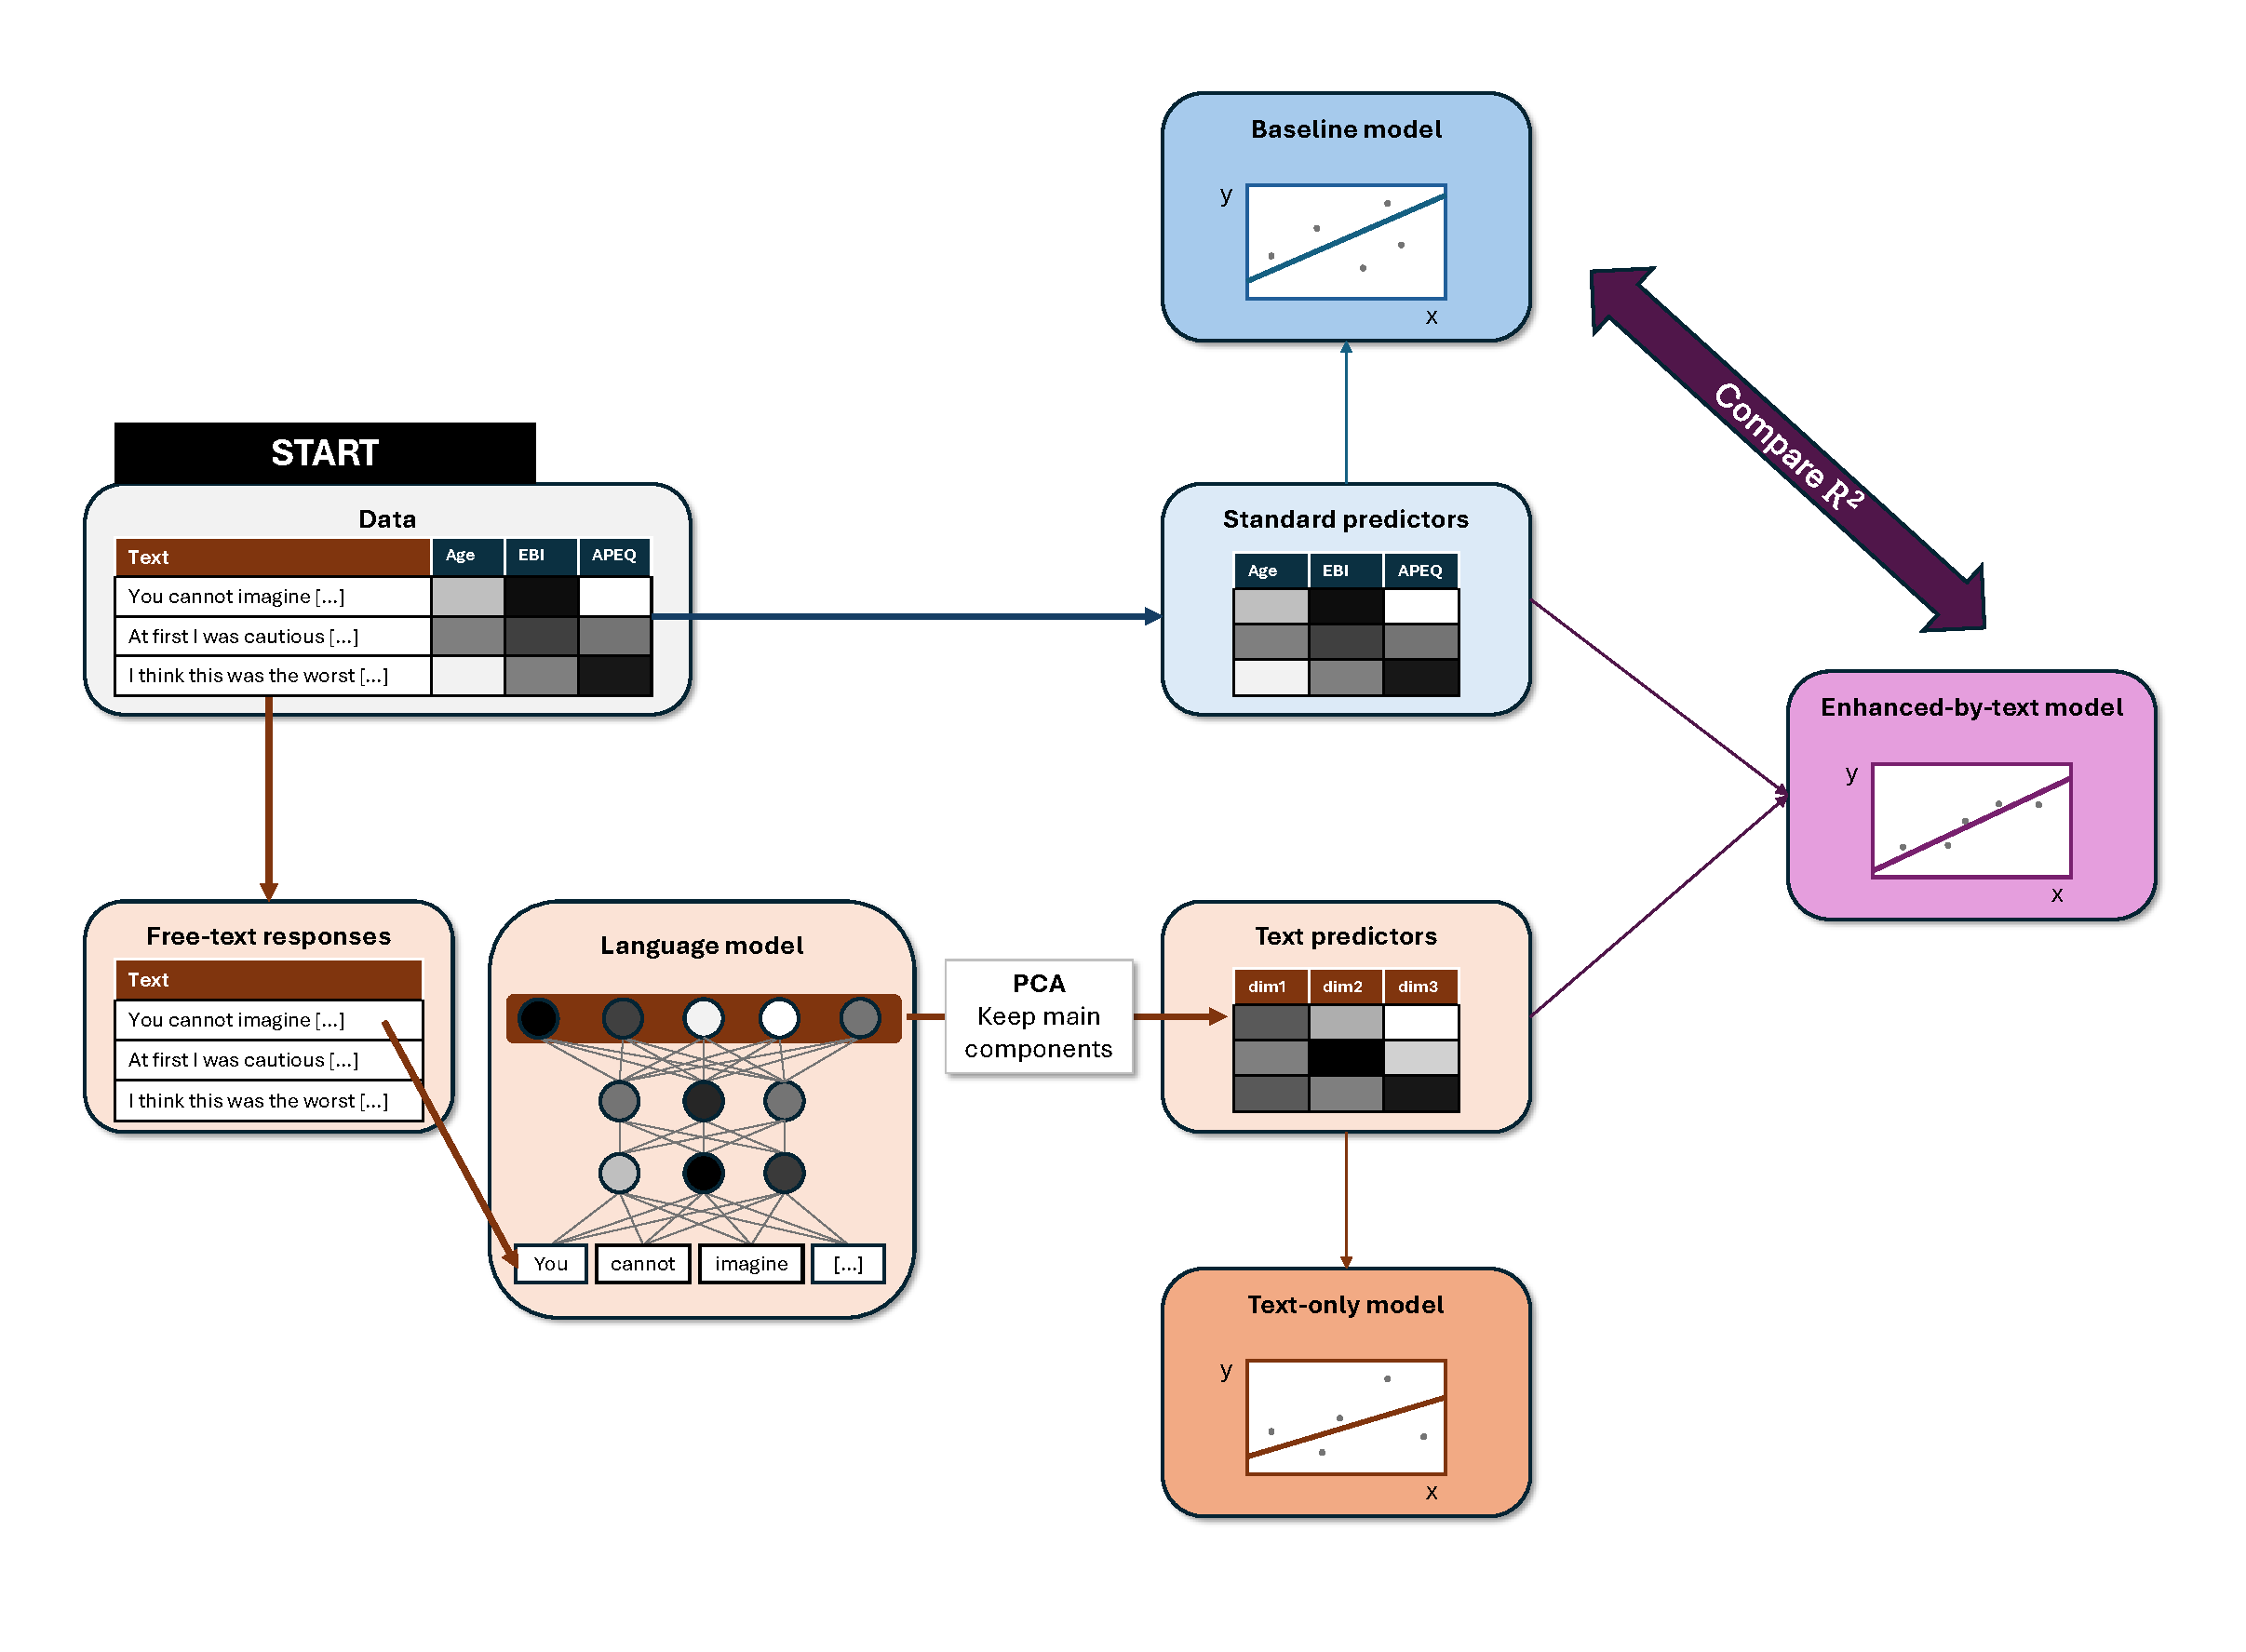
\includegraphics[width=1\linewidth]{workflow.pdf}
    \caption{Simplified overview of the overall analysis pipeline employed in our study}
    \label{fig:pipeline}
\end{figure}

\subsection{Datasets}

A summary overview of all datasets is provided in Table~\ref{tab:results_summary}.


\begin{table}[!htbp]
\small\renewcommand{\arraystretch}{0.9}%

    \caption{Overview of the datasets and main results for all outcome variables considered here. \change{$R^2$ values are cross-validated (held-out) $R^2$ from the repeated nested cross-validation, with \res{set.nprin} PCA components per free-text response. The baseline + text model contains all free-text responses of the dataset (the pre-specified test); $\Delta R^2$ is tested with the corrected repeated $k$-fold $t$-test.}}

    \centering
    \begin{threeparttable}

    % generated by R/export_tex.R -- do not edit by hand.
\begin{tabular}{llllll}
\hline
dataset & \multicolumn{2}{c}{APEQ} & \multicolumn{1}{c}{GCMQ} & \multicolumn{2}{c}{PTSD} \\
\hline
outcome & WHO-5 & AAQ-II & WEMWBS & PCL-5 & PTGI \\
\hdashline
$N$ analysed & \multicolumn{2}{c}{\synth{958}} & \synth{605} & \synth{232} & \synth{229} \\
\# free-text responses & \multicolumn{2}{c}{\synth{1}} & \synth{2} & \multicolumn{2}{c}{\synth{3}} \\
\# other predictors & \multicolumn{2}{c}{\synth{20}} & \synth{45} & \multicolumn{2}{c}{\synth{36}} \\
-- demographic & \multicolumn{2}{c}{\synth{4}} & \synth{14} & \multicolumn{2}{c}{\synth{5}} \\
-- setting & \multicolumn{2}{c}{\synth{8}} & \synth{19} & \multicolumn{2}{c}{\synth{25}} \\
-- questionnaires & \multicolumn{2}{c}{\synth{8}} & \synth{12} & \multicolumn{2}{c}{\synth{6}} \\
\hdashline
baseline model $R^2$ & \synth{.369} & \synth{.399} & \synth{.207} & \synth{.325} & \synth{.317} \\
baseline + text model $R^2$ & \synth{.411} & \synth{.432} & \synth{.205} & \synth{.449} & \synth{.309} \\
$\Delta R^2$ & \synth{.042} & \synth{.033} & \synth{\ensuremath{-}.002} & \synth{.124} & \synth{\ensuremath{-}.008} \\
-- 95\% CI & \synth{[.018, .065]} & \synth{[.012, .054]} & \synth{[\ensuremath{-}.015, .011]} & \synth{[.037, .212]} & \synth{[\ensuremath{-}.033, .017]} \\
-- $t$ (df) & \synth{3.48 (99)} & \synth{3.08 (99)} & \synth{\ensuremath{-}0.33 (99)} & \synth{2.81 (99)} & \synth{\ensuremath{-}0.65 (99)} \\
-- $p$ & \synth{$<$ .001} & \synth{.003} & \synth{.741} & \synth{.006} & \synth{.517} \\
text-only model $R^2$ & \synth{.220} & \synth{.196} & \synth{.030} & \synth{.180} & \synth{.044} \\
\hline
\end{tabular}


\begin{tablenotes}[flushleft]
\small
\item \change{\textit{Note.}\\ \textit{APEQ}: Acceptance/Avoidance-Promoting Experiences Questionnaire, \cite{wolff2022acceptance}, \textit{WHO-5}: WHO well-being index , \textit{AAQ-II}: Acceptance and Action
Questionnaire II\\ \textit{GCMQ}: General Change Mechanisms Questionnaire \cite{wolff2024measuring}, \textit{WEMWBS}: Warwick-Edinburgh Mental Wellbeing Scale, \\ \textit{PTSD}: Post-traumatic stress disorder symptoms \cite{evens2026post}, \textit{PCL-5}: PTSD Checklist for DSM-5, \textit{PTGI}:  Post-Traumatic Growth Inventory.}
\end{tablenotes}


\end{threeparttable}
    \label{tab:results_summary}
\end{table}


\subsubsection{APEQ}

The first dataset was collected by \textcite{wolff2022acceptance}, originally for the creation and validation of the \emph{Acceptance/Avoidance-Promoting Experiences Questionnaire} (APEQ), a questionnaire \change{designed to measure motivational, emotional, cognitive aspects of (acceptance- and avoidance-related) psychedelic experiences}.
\textcite{wolff2022acceptance} collected data from \change{\res{n.apeq.raw} participants; after applying the exclusion criteria of the original study, data from \res{n.apeq.after-exclusion} participants remain (\res{n.apeq.after-exclusion-language.eng} English- and \res{n.apeq.after-exclusion-language.ger} German-speaking),} who each reported on one psychedelic experience (clearly discernible psychoactive effects) following the use of different substances (LSD, psilocybin, mescaline, or ayahuasca). Participants were instructed that both positive and negative experiences could be reported on.

\paragraph{Outcome variables:} In the analysis of the APEQ data, our main outcome variable of interest is the  change in subjective well-being (assessed via the WHO-5 well-being index, \cite{topp2015}) from before to after the psychedelic experience. Both the "before" and "after" rating were assessed retrospectively by the participants, \change{and the change score was computed as the difference between the two scores}. Subjective well-being is an ideal outcome variable in this setting: On the one hand, it is a very general variable that is influenced by many different factors \change{\parencite{dolan2008we}}; on the other hand, as a measure of general life satisfaction, it is of immediate practical importance to practitioners and patients.


As a secondary outcome variable, we also considered difference in psychological flexibility before and after the psychedelic experience, which is the variable which \textcite{wolff2022acceptance} used to validate the APEQ questionnaire. Both the "before" and "after" rating were assessed retrospectively by the participants via the AAQ-II (Acceptance and Action Questionnaire II; \cite{bond2011preliminary,hoyer2013psychologische}). \change{Note that the AAQ is coded so that higher values indicate \emph{less flexibility}. Consequently, negative changes indicate an \emph{increase} in flexibility.  This is also reflected in the strong negative correlation ($r = \res{apeq.cor.who.aaq}$) between WHO-5 differences and AAQ-II differences in the data. We will note this again in the respective results sections.}

\paragraph{Free-text responses.} After questions on demographic data and mental health issues/diagnoses, participants were asked to describe the psychedelic experience in a free-text format, either in English or German. This free-text data is available from \res{n.apeq.with-text} participants (\res{n.apeq.with-text-language.eng} English-speaking, \res{n.apeq.with-text-language.ger} German-speaking). Only data from these \res{n.apeq.with-text} participants is passed on to further analysis.

\paragraph{Other predictor variables.} In addition to the free-text responses, participants answered a series of questionnaires (see  \cite{wolff2022acceptance} for detailed information). Here, we consider the following relevant variables:
\begin{itemize}
    \item \textbf{Demographic:} age, gender [female, male, other], education level [primary, intermediate, higher]; native language [English, German]
    \item \textbf{Setting (of the psychedelic experience):} substance taken, subjective strength of the dose, \change{subjective strength of the effects}, duration of the episode, valence of the episode, \change{and retrospective appraisal of the episode (how positive/negative it was judged in hindsight)}, mood, preparedness
    \item \textbf{Questionnaire data:} EBI (Emotional Breakthrough Inventory, \cite{roseman2019emotional}), CEQ (Challenging Experience Questionnaire, \cite{barrett2016challenging,dworatzyk2022phenomenological}), the  APEQ \parencite{wolff2022acceptance} subscales     APEQ-AVE (avoidance-related experience) and APEQ-ACE (acceptance-related experience) \change{plus their interaction term \parencite{wolff2022acceptance}}, \change{as well as Therapeutic use motives, Hedonic use motives, and Escapist use motives (factor scores from an additional questionnaire, \cite{wolff2022acceptance}).} 
    
\end{itemize}


\subsubsection{GCMQ}

The second dataset was collected by \textcite{wolff2024measuring} for the creation and validation of the \emph{General Change Mechanisms Questionnaire} (GCMQ). This questionnaire is \change{intended to measure psychotherapeutic or psychotherapy-like aspects of psychedelic experiences in the sense of five well-established general change mechanisms of psychotherapy:} resource activation, therapeutic relationship, problem actuation, clarification, and mastery.\textcite{wolff2024measuring} collected data from \res{n.gcmq.raw-language.eng} English-speaking and \res{n.gcmq.raw-language.ger} German-speaking participants, who each were asked to select one memorable psychedelic experience (negative or positive) to report on, and then provided responses on a series of questions and questionnaires. 


\paragraph{Outcome variables:} In the GCMQ data, our outcome variable is mental well-being as assessed via the WEMWBS (Warwick-Edinburgh Mental Wellbeing
Scale; \cite{tennant2007warwick}), the same variable used in the validation study by \textcite{wolff2024measuring}. Note that, in contrast to the outcome variables in the APEQ data, this is not a change score from before to after the psychedelic experience, but instead a state assessment of mental well-being in the two weeks prior to data collection.


\paragraph{Free-text responses.} In free-text responses, participants described the impact of the psychedelic experience on (a) their handling of stressful events, and  (b) on their mental health. We thus have two different free-text responses available here, describing related but potentially different topics. Such free-text data is available from \res{n.gcmq.with-text} participants (\res{n.gcmq.with-text-language.eng} English-speaking, \res{n.gcmq.with-text-language.ger} German-speaking; roughly 2/3 of the dataset used for the APEQ analysis). Only data from these \res{n.gcmq.with-text} participants is passed on to further analysis.


\paragraph{Other predictor variables.} In addition to the free-text responses, participants answered a series of questionnaires (see  \cite{wolff2024measuring} for detailed information). Here, we consider the following relevant variables:

\begin{itemize}

    \item \textbf{Demographic:} age, gender [female, male, other], education level [primary, intermediate, higher]; native language [English, German]; as well as mental disorder diagnosis [yes, no], which was further differentiated by the type of diagnosis (all yes/no: depression, anxiety, ADHD, PTSD, addiction, mania, psychosis, other) and the total number of stressful life events in the past five years (cumSLE; \cite{seery2010whatever}).  


    \item \textbf{Setting (of the psychedelic experience):} general setting (each yes/no: nature, party, therapy, ceremony), substance taken, subjective strength of the dose,  subjective clarity of memory for the episode, valence and retrospective appraisal of the episode, suitability of the setting for having a psychedelic experience, as well as concomitant use of another substance during the experience (each yes/no: \change{none,} cannabis, alcohol, entactogens, dissociatives, stimulants, benzodiazepines, opiates, other). 

    
    \item \textbf{Questionnaire data:} EBI; CEQ; ASC-OBE (the Oceanic Boundlessness scale of the Altered States of Consciousness Questionnaire ASC; \cite{dittrich1998standardized,studerus2010psychometric}); the \change{APEQ subscales
    APEQ-AVE and APEQ-ACE;} Therapeutic use motives, Hedonic use motives, Escapist use motives; and  the following GCMQ subscales \parencite{wolff2024measuring}: GCMQ-RA (resource activation), GCMQ-PA (problem actuation), GCMQ-CL (clarification), GCMQ-MA (mastery). The GCMQ-RE (relationship) subscale was dropped from analysis because no scores were available for \res{n.gcmq.gcmqre.missing} of the \res{n.gcmq.with-text} participants.
    
\end{itemize}


\subsubsection{PTSD}

The third dataset -- here labelled \emph{PTSD} -- was collected by \textcite{evens2026post} as a naturalistic survey study to investigate the development of post-traumatic stress disorder (PTSD) symptoms following psychedelic substance use. 


\synthmismatch{\change{A total of 1,195 volunteers began the survey and 512 provided informed consent to participate. Of these, 269 participants were excluded for the following reasons: not meeting inclusion criteria (n = 90), discontinuation of the survey before completing the PCL-5 items (n = 176), free-text responses indicating a lack of genuine participation (e.g., “just reading”; n = 2), or exceeding the recommended relative speed index cut-off (> 2) without any indication of engagement in free-text comments (n = 1).}} From \textcite{evens2026post} we thus use data from \res{n.ptsd.raw-language.eng} English-speaking and \res{n.ptsd.raw-language.ger} German-speaking participants who reported distressing experiences during or beyond the acute phase. Thus, the sample constitutes a selective subset of psychedelic substance users. Participants were asked to report on this ``particularly challenging or traumatic psychedelic experience'', and additionally provided responses on a series of questions and questionnaires. 


\paragraph{Outcome variables:} In the PTSD data, our main outcome variable is the sum score of the PCL-5 (PTSD Checklist for DSM-5; \cite{blevins2015posttraumatic,kruger2017german}), a questionnaire to assess the severity of PTSD symptoms as defined per the DSM-5 criteria. In a modification of the original instructions, participants were asked to rate their symptoms not over the past month, but specifically with reference to the month they found most challenging following their psychedelic experience. \change{PCL-5 scores are available from all \res{n.ptsd.pcl.with-outcome} participants, of which \res{n.ptsd.pcl.analysed} are analysed (\res{n.ptsd.pcl.excluded-text} participants left at least one of the free-text responses empty, see below; for \res{n.ptsd.pcl.excluded-predictor} participant, one of the other predictors is missing).}

As an additional outcome variable, we also considered the sum score of the PTGI (Post-Traumatic Growth Inventory; \cite{maercker2001posttraumatic,tedeschi2004posttraumatic}), a questionnaire assessing \emph{positive} psychological change following traumatic experiences. \change{PTGI scores are only available from \res{n.ptsd.ptgi.with-outcome} participants, of which \res{n.ptsd.ptgi.analysed} are analysed (for \res{n.ptsd.ptgi.excluded-predictor} participant, one of the other predictors is missing).}


\paragraph{Free-text responses.} \change{Participants were asked three questions to which they were instructed to provide free-text responses: 1) \textit{Acute Symptoms.} Please describe the challenging or traumatic experience you had with psychedelics. Kindly elaborate on the encounters you had during the acute substance effects. 2) \textit{Post-acute Symptoms.} Please describe all persistent symptoms or difficulties in the days, weeks, months, or years following the challenging or traumatic experience you had with psychedelics.
3) \textit{Treatment.} Please provide a detailed description of the attempts you have made so far to address the symptoms. What have you found helpful, and what have you found to be less helpful or even harmful?} \change{Empty responses were treated as missing data (\res{n.ptsd.empty-acute} acute, \res{n.ptsd.empty-post} post-acute, and \res{n.ptsd.empty-treat} treatment responses). As all models for one outcome variable were estimated on the same participants, participants with an empty response were not included in the analyses.}


\paragraph{Other predictor variables.} In addition to the free-text responses, participants answered a series of questionnaires (see  \change{\cite{evens2026post}} for detailed information). Here, we consider the following relevant variables:

\begin{itemize}

    \item \textbf{Demographic:} age, gender [female, male, \change{non-binary,} other]; native language [English, German]; country of residence \change{[countries listed $\le 5$ times among the participants with the respective outcome score were pooled into a single "other" category]}; CASMIN education level \parencite{Brauns2003CASMIN} \change{[levels listed $\le 5$ times among the participants with the respective outcome score were pooled into a single "other" category]}


    \item \textbf{Setting (of the psychedelic experience):} Substance taken \change{(19 variables in the datasets, 7 of which are general variables on the number of substances and how they were used, and 12 dummy variables for different substances such as LSD, DMT, ...; see \cite{evens2026post})}, subjective strength of the dose, subjective clarity of memory for the episode, duration of the episode, valence as well as retrospective appraisal of the episode, how challenging the episode was perceived
    
    \item \textbf{Questionnaire data:} CEQ; APEQ-ACE; APEQ-AVE; \change{Self-exploration use motives, Hedonic use motives, and Escapist use motives \parencite{evens2026post}}
    
\end{itemize}


\subsection{Text embeddings}

The bottom part (orange track) in Figure~\ref{fig:pipeline} illustrates the text embedding pipeline schematically. 

\synthmismatch{After minimal text cleaning \change{in the raw data (removal of names and personal contact data; removal of three random character strings)},} we extracted sentence embeddings \parencite{reimers2019sentence} for the free-text responses  using the R package \emph{reticulate} \parencite{reticulate}. In particular, as free-text responses are available in different languages (German and English), we selected the \emph{intfloat/multilingual-e5-large} model \parencite{wang2024multilingual} from the Hugging Face platform (\url{https://huggingface.co/intfloat/multilingual-e5-large}), which produces 1,024-dimensional embeddings for each text in 24 model layers. \synthmismatch{A robustness check with the \emph{BAAI/bge-m3} model \parencite{bge-m3} that arrives at very similar results as the main analysis is presented in the Supplementary Material.} As open model weights are downloaded from Hugging Face to a local machine for extracting text embeddings, the model runs fully offline, no third-party API is involved, and participant responses are not sent to any third party as part of this process.

In datasets where we have multiple free-text responses (2 in the GCMQ data: events and health; 3 in the PTSD data: acute, post-acute, and treat), we embedded each of them separately.  With the model's context length of 512 tokens, almost all the free-text responses could be fully embedded; longer responses were truncated\footnote{Since the bge-m3 has a longer context length, all responses could be fully embedded there; see the Supplementary Material}. In line with the  multilingual-e5-large model setup, the prefix ``passage:'' was \change{prepended} to all responses before extracting the embeddings\change{ (for comparability, this was also done for the bge-m3 model, so that the two analyses differ only in the embedding model)}. Following the conventional approach (e.g., \cite{kjell2023text}), we used the embeddings in the final hidden layer of the model (before the output layer), where the embeddings are fully contextualized and make use of all learned weights of the model, for further analysis\change{. As implemented in the \emph{sentence-transformers} library, a single embedding per response was obtained by averaging over the token embeddings (multilingual-e5-large) or by taking the embedding of the initial [CLS] token (bge-m3), and normalized to unit length}.

Sentence transformers produce high-dimensional representations to be able to adequately represent the vast variety of possible text (and their semantic content) that can occur in natural language. However, free-text responses describing psychedelic experiences will usually not cover the whole range of possible semantic content, and so 1,024 distinct numerical predictors for each text will not be required in our setup. In addition, text embedding dimensions can be highly collinear, especially for thematically related texts. We therefore ran a Principal Component Analysis (PCA) over all text embeddings from an individual set of free-text responses, and only retained the \res{set.nprin} first principal components. This number was held constant across all analyses for consistency. A parameter sweep for different numbers of principal components is presented in the Supplementary Material. \change{Note that the PCA ran \emph{within} the folds of the cross-validation (next section).}


\subsection{\change{Analysis pipeline: Elastic net with cross-validation}}

The central question of the present study is whether we can gain additional predictive accuracy in statistical analyses by considering  the information provided in participants' free-text responses, in the form of automatically-extracted text embeddings without any additional (human) annotation. Thus, our main focus  lies on prediction, rather than interpretations of individual model parameter estimates \parencite{yarkoni2017choosing,shmueli2010explain} -- especially since the dimensions of text embeddings are usually not directly interpretable but require additional analyses (e.g., \cite{kjell2023text,Kjell2019}). Accordingly, our metric of interest is incremental validity -- that is, increases in variance explained $\Delta R^2$ when predictor variables from text embeddings are included as \emph{additional} predictors in cross-validated regression models that are designed to counteract over-fitting.    


For a schematic overview of the analysis pipeline, see again Figure~\ref{fig:pipeline}. To assess the added predictive accuracy brought about by free-text data, we estimated nested regression models for each outcome variable: The main analysis relies on a baseline model containing what has been defined in the Method sections as ``other predictor variables'' (the upper, blue track of Figure~\ref{fig:pipeline}), and ``extended-by-text'' models that additionally include the \res{set.nprin} text-embedding principal components for a specific free-text response (the rightmost, purple part of Figure~\ref{fig:pipeline}, combining the blue and orange tracks). 


Depending on the number $k$ of free-text responses in a dataset, we will have a nested hierarchy of such extended-by-text models, as will be described in detail in the individual sections below. All regression models were estimated using elastic net regression \parencite{zou2005regularization}. Elastic net is a regularization technique that combines ridge and lasso penalties to shrink (ridge) and, where appropriate, eliminate (lasso) coefficients. This renders \change{it} useful to counter-act overfitting in datasets with many, potentially correlated predictors. 

Model performance for each elastic net model was evaluated using \change{repeated nested} cross-validation \change{using the R package \emph{caret} \parencite{caret}}: \change{In the outer loop, the data were split into \res{set.folds} folds;} for each fold, the model was trained and model coefficients estimated on 90\% of the data, and the resulting model was then used to generate  predictions for the remaining 10\% held-out data which the model has not seen during training. \change{The PCA on the text embedding dimensions ran on the training data only, and the coefficients from the training set were then used to project the embeddings of the test set into the same lower-dimensional space (i.e., perform dimensionality reduction).} This process repeated across all folds\change{, and the whole procedure was repeated \res{set.repeats} times with different random assignments of participants to folds (i.e., \res{set.repeats}~$\times$~\res{set.folds} outer folds in total)}. The  \change{squared correlation between predicted and observed values in each held-out fold, averaged over all outer folds,} constitutes the cross-validated (\change{held-out}) $R^2$ \change{\parencite{caret}}. The elastic net hyperparameters (the mixing parameter $\alpha$ and penalty strength $\lambda$) were tuned via grid search (hyperparameter ranges: $\alpha \in [0, 1]$, \change{\res{set.alpha.n} values in steps of 0.1}; $\lambda \in [\res{set.lambda.min}, \res{set.lambda.max}]$, \res{set.lambda.n} log-spaced values)\change{, in an inner loop: Within each outer training set, we ran a \res{set.innerfolds}-fold cross-validation (again with the PCA computed on the inner training data only), selected the combination of $\alpha$ and $\lambda$ yielding the highest inner cross-validated $R^2$, and then re-fitted the model with these values on the whole outer training set. The held-out data of an outer fold were thus used neither for estimating the coefficients nor for selecting the hyperparameters, so that the cross-validated $R^2$ is not inflated by the hyperparameter selection \parencite{varma2006bias}}. Note that  \emph{different} values of $\alpha$ and $\lambda$ can thus be applied for the baseline model and the extended-by-text models \change{(as well as in different outer folds; we report their median across the outer folds)}. As our aim is to assess how much predictive information can be gauged from the predictor variables, and not how the regression models perform under exactly the same hyperparameter settings, this choice aligns with our study objectives. As noted above, the difference in cross-validated $R^2$ between the model with and without text-embedding predictors ($\Delta R^2$, also referred to as \emph{incremental validity}; \cite{hunsley2003incremental, sechrest1963incremental} ) serves as the index of the added predictive value of the free-text data.

\change{To test whether the free-text data reliably increase predictive accuracy, we compared each extended-by-text model with the baseline model on the same outer folds (all models for one outcome variable were evaluated on identical outer and inner folds). For each outer fold $j$, we computed the difference $d_j$ between the held-out $R^2$ of the two models; $\Delta R^2$ is the mean of these $J = \res{set.repeats} \times \res{set.folds}$ differences. Since the training sets of different folds overlap, the $d_j$ are not independent, and a standard paired $t$-test would underestimate their variance. We therefore used a corrected repeated $k$-fold $t$-test \parencite{nadeau2003inference,bouckaert2004evaluating}, and report 95\% confidence intervals based on the same corrected standard error. In datasets with more than one free-text response, we pre-specified the extended-by-text model containing \emph{all} free-text responses as the test of incremental validity; the models with other combinations of responses are reported descriptively (their $p$-values are not corrected for multiple comparisons). The hyperparameter sweep over the number of principal components (Supplementary Material)\change{, all qualitative examples reported below, and the text signal in the overlap analysis (Table~\ref{tab:overlap})} are based on a single (non-repeated, non-nested) \res{set.folds}-fold cross-validation run.}


\section{Results}


A summary of the main results for all outcome variables is provided in Table~\ref{tab:results_summary}


\subsection{APEQ}

\subsubsection{Quantitative analysis.} {For the well-being difference (WHO-5) in the APEQ data, we obtain a cross-validated $R^2 = \res{e5.apeq.who.none.r2}$ for the baseline model (\change{median tuned hyperparameters across the outer folds:} $\alpha = \res{e5.apeq.who.none.alpha}$, $\lambda = \res{e5.apeq.who.none.lambda}$), and  a cross-validated $R^2 = \res{e5.apeq.who.text.r2}$ for the extended-by-text model ($\alpha = \res{e5.apeq.who.text.alpha}$, $\lambda = \res{e5.apeq.who.text.lambda}$). Consequently, we find a  $\Delta R^2 = \res{e5.apeq.who.text.delta}$ between the two models \change{(95\% CI [\res{e5.apeq.who.text.cilo}, \res{e5.apeq.who.text.cihi}], $t(\res{e5.apeq.who.text.df}) = \res{e5.apeq.who.text.t}$, \res{e5.apeq.who.text.p})}: adding the information from the free-text data in form of text embeddings increases the variance explained by \res{e5.apeq.who.text.deltapct}\% in absolute terms} (and \res{e5.apeq.who.text.relgain}\% in relative terms, starting from the baseline model's $R^2 = \res{e5.apeq.who.none.r2}$). For an elastic net model that \emph{only} takes the \res{set.nprin} text-embedding principal components as input, we already obtain a cross-validated $R^2 = \res{e5.apeq.who.textonly.r2}$.

{For the change in psychological flexibility (AAQ-II), we obtain a cross-validated $R^2 = \res{e5.apeq.aaq.none.r2}$ for the baseline model (\change{median} $\alpha = \res{e5.apeq.aaq.none.alpha}$, $\lambda = \res{e5.apeq.aaq.none.lambda}$),  a cross-validated $R^2 = \res{e5.apeq.aaq.text.r2}$ for the extended-by-text model (\change{median} $\alpha = \res{e5.apeq.aaq.text.alpha}$, $\lambda = \res{e5.apeq.aaq.text.lambda}$), and consequently a $\Delta R^2 = \res{e5.apeq.aaq.text.delta}$} \change{(95\% CI [\res{e5.apeq.aaq.text.cilo}, \res{e5.apeq.aaq.text.cihi}], $t(\res{e5.apeq.aaq.text.df}) = \res{e5.apeq.aaq.text.t}$, \res{e5.apeq.aaq.text.p};} an increase of \res{e5.apeq.aaq.text.deltapct}\% in absolute terms and of \res{e5.apeq.aaq.text.relgain}\% in relative terms). Here, an elastic net model that \emph{only} takes the \res{set.nprin} text-embedding principal components as input achieves a cross-validated $R^2 = \res{e5.apeq.aaq.textonly.r2}$.


These results already indicate that the free-text responses contain information not captured in the other predictor variables. To quantify the shared variance between the free-text data and the other predictors, \change{we regressed each of the other predictor variables on the \res{set.nprin} text-embedding principal components  (Table~\ref{tab:overlap}, for all three datasets, using $^{b}$Tjur's $R^2$ for binary variables \cite{tjur2009coefficients}). The  overlap between text data and the other predictors is small to moderate: \synthmismatch{no single predictor shares more than \res{e5.apeq.overlap.factor1-therapeutic} of its variance with the text components}, and most values are below .10. The texts partially tap into information assessed via the questionnaires, such as therapeutic use motives, acceptance- and avoidance-related experiences, the subjective experience of overcoming emotional challenges by substance use, as well as the retrospective appraisal of the experience. Overlap with the other setting dimensions is consistently small. Moreover, the other predictors together explain only about a third of the outcome-relevant information extracted from the texts (text signal, e.g., \res{e5.apeq.who.textsignal.r2} for WHO-5 and \res{e5.ptsd.pcl.textsignal.r2} for PCL-5). However, it is also evident that information encoded in the text data (a) goes far beyond what these questionnaires measure, and (b) this additional information is useful for predicting differences in the outcome variables.  
 }


\begin{table}[!htbp]
	\caption{Shared variance between the text embeddings and the other predictor variables.}
	\centering
	\renewcommand{\baselinestretch}{1}\normalsize
	\begin{threeparttable}
		% generated by R/export_tex.R -- do not edit by hand.
\small\renewcommand{\arraystretch}{0.88}%
\begin{tabular}{lccc}
\hline
 & APEQ & GCMQ (health) & PTSD (post) \\
$N$ & \synth{958} & \synth{605} & \synth{232} \\
\hline
\multicolumn{4}{l}{\textit{Demographic}} \\
\quad Age & \synth{.010} & \synth{.018} & \synth{\ensuremath{-}.001} \\
\quad Stressful life events & -- & \synth{.033} & -- \\
\quad Mental disorder diagnosis & -- & \synth{.039}$^{b}$ & -- \\
\quad Depression diagnosis & -- & \synth{.034}$^{b}$ & -- \\
\multicolumn{4}{l}{\textit{Setting}} \\
\quad Dose & \synth{.010} & \synth{\ensuremath{-}.004} & \synth{\ensuremath{-}.021} \\
\quad Strength & \synth{\ensuremath{-}.005} & -- & -- \\
\quad Valence & \synth{\ensuremath{-}.001} & \synth{.038} & \synth{\ensuremath{-}.027} \\
\quad Retrospective appraisal & \synth{.113} & \synth{.029} & \synth{.078} \\
\quad Clarity of memory & -- & \synth{.009} & \synth{.050} \\
\quad Duration & \synth{.004} & -- & \synth{\ensuremath{-}.001} \\
\quad Mood & \synth{.010} & -- & -- \\
\quad Preparedness & \synth{.022} & -- & -- \\
\quad Challenge & -- & -- & \synth{\ensuremath{-}.055} \\
\quad Suitability of setting & -- & \synth{.024} & -- \\
\quad Setting: nature & -- & \synth{.034}$^{b}$ & -- \\
\quad No concomitant substance & -- & \synth{.035}$^{b}$ & -- \\
\quad Number of psychedelics & -- & -- & \synth{.036} \\
\quad Number of other substances & -- & -- & \synth{\ensuremath{-}.010} \\
\quad Number of substances (total) & -- & -- & \synth{.039} \\
\multicolumn{4}{l}{\textit{Questionnaires}} \\
\quad Therapeutic use motives & \synth{.159} & \synth{.087} & -- \\
\quad Self-exploration use motives & -- & -- & \synth{.018} \\
\quad Escapist use motives & \synth{\ensuremath{-}.009} & \synth{.072} & \synth{\ensuremath{-}.031} \\
\quad Hedonic use motives & \synth{\ensuremath{-}.010} & \synth{\ensuremath{-}.001} & \synth{.006} \\
\quad APEQ-ACE & \synth{.213} & \synth{\ensuremath{-}.006} & \synth{\ensuremath{-}.004} \\
\quad APEQ-AVE & \synth{.011} & \synth{.019} & \synth{.007} \\
\quad EBI & \synth{.101} & \synth{.000} & -- \\
\quad CEQ & \synth{.053} & \synth{.023} & \synth{.022} \\
\quad ASC-OBE & -- & \synth{.076} & -- \\
\quad GCMQ-RA & -- & \synth{.075} & -- \\
\quad GCMQ-PA & -- & \synth{\ensuremath{-}.003} & -- \\
\quad GCMQ-CL & -- & \synth{.036} & -- \\
\quad GCMQ-MA & -- & \synth{.003} & -- \\
\hdashline
rare binary predictors (dropped) & \synth{0} & \synth{18} & \synth{14} \\
categorical predictors (not used) & \synth{3} & \synth{3} & \synth{5} \\
\hdashline
text signal$^{t}$, main outcome & \synth{.339} (WHO-5) & \synth{.606} (WEMWBS) & \synth{.233} (PCL-5) \\
text signal$^{t}$, secondary outcome & \synth{.336} (AAQ-II) & -- & \synth{.010} (PTGI) \\
\hline
\end{tabular}

		\begin{tablenotes}[flushleft]
			\small
			\item \textit{Note.} Values are the variance in each predictor variable explained by the first \res{set.nprin} principal components of the free-text response indicated in the header (the response with the largest incremental validity in each dataset\change{, in the single cross-validation run}; \change{for this descriptive analysis, the PCA was computed on the whole analysis sample rather than within cross-validation folds}): adjusted $R^2$ from linear regression for continuous variables; $^{b}$Tjur's $R^2$ from logistic regression for binary variables. Binary variables with fewer than \res{set.overlap.minn} participants in either category, categorical variables with more than two levels, and the response language were not considered. $^{t}$Text signal: adjusted $R^2$ of a linear regression of the held-out predictions of the text-only model \change{(single \res{set.folds}-fold cross-validation run)} on all other predictor variables.
		\end{tablenotes}
	\end{threeparttable}
	\label{tab:overlap}
\end{table}


\subsubsection{Qualitative examples.} To provide some qualitative impressions as to what predictive pieces of information the free-text responses capture that the questionnaires missed, we predicted each participant's outcome (\change{held-out}) from the baseline model and from the extended-by-text model. The difference in a participant's residual between the two models is a index for the predictive improvement brought about by the inclusion of text data; the difference in the predicted value for that person shows the ``direction of the effect''. The fifteen responses with the highest improvement are displayed in Table~\ref{tab:examples_APEQ}. Keep in mind that interpretations of such examples are inherently qualitative, subjective, and do not necessarily reflect patterns in the entire dataset (which is exactly why the main analysis avoids human annotation) -- they are intended to serve as illustrations. 

That being said, for differences in well-being (WHO-5), the examples in Table~\ref{tab:examples_APEQ} suggest quite clearly that the best-improving positive shifts are found where the free-text responses describe positive emotions following the substance use: relaxation, intense positive feelings of happiness, symptoms relief in affective disorders,  and general life satisfaction. This pattern is especially interesting given the very low correlation between the text information and the valence \emph{of the acute effects}. On the other hand, the best-improving negative shifts (that is, decreases in the outcome variable)  are found when the free-text responses describe insights and (meta-)cognitive processes, especially evaluations and judgments: increased awareness for oneself and ones own mental states, as well as the (social) environment. So interestingly, the free-text responses associated with positive and negative shifts are not polar opposites on one semantic dimension. 


\begin{table}[!htbp]
\centering
\caption{The \res{set.examples} responses in the APEQ dataset for which \change{held-out} prediction of change in well-being (WHO-5) improved most when text-embedding predictors were added (\emph{improvement}), alongside the change in the predicted value (\emph{shift}). Negative shift values are displayed in boldface. } 
\label{tab:examples_APEQ}
\scriptsize
\begin{threeparttable}
\begin{tabular}{p{12cm}rr}
 \hline
Response & Improvement & Shift \\
  \hline
% generated by R/export_tex.R -- do not edit by hand. Rows only (incl. the final \hline); response type: text; English version: 4 response(s) translated from translations/example_responses_en.csv, marked with \dagger
\synth{It was very confusing and I didn't understand much of what happened.} & \synth{2.75} & \textbf{\synth{\ensuremath{-}2.75}} \\
\synth{The depression is gone. Simply gone. I can hardly believe it myself.$^{\dagger}$} & \synth{2.49} & \synth{2.49} \\
\synth{Life is good} & \synth{2.22} & \synth{2.22} \\
\synth{I became aware of how, in conversations, I often just wait for my turn to talk instead of listening. I also recognised patterns in my family that repeat over generations, e.g. that we never talk about feelings. This has been on my mind a lot ever since.$^{\dagger}$} & \synth{2.21} & \textbf{\synth{\ensuremath{-}2.21}} \\
\synth{It made me notice how much I interrupt people and how little I actually listen. I'm working on it, it's embarrassing.} & \synth{2.15} & \textbf{\synth{\ensuremath{-}2.15}} \\
\synth{The trip made me take a long hard look at how I behave when I'm drunk. I didn't like what I saw.} & \synth{2.10} & \textbf{\synth{\ensuremath{-}2.10}} \\
\synth{Happiness. Relief. Love.} & \synth{2.07} & \synth{2.07} \\
\synth{Since the trip I've been very aware of my negative thinking patterns at work. I keep thinking everyone is more competent than me and I notice now how this affects what I say in meetings, or rather what I don't say. It's been eye opening but I haven't managed to change it yet.} & \synth{2.05} & \textbf{\synth{\ensuremath{-}2.05}} \\
\synth{I noticed during the experience that I constantly evaluate myself, like there's a judge in my head scoring everything I do.} & \synth{2.05} & \textbf{\synth{\ensuremath{-}2.05}} \\
\synth{For the first time I consciously noticed how much I judge others, and that these judgements usually say more about me than about the others.$^{\dagger}$} & \synth{2.04} & \textbf{\synth{\ensuremath{-}2.04}} \\
\synth{I feel reborn. The depression that was with me for years has almost disappeared. I can laugh again, fall in love, make plans. I am so grateful.$^{\dagger}$} & \synth{2.04} & \synth{2.04} \\
\synth{So much joy} & \synth{2.04} & \synth{2.04} \\
\synth{It was scary but I learned a lot about my fears} & \synth{2.01} & \textbf{\synth{\ensuremath{-}2.01}} \\
\synth{made me reflect on the choices I've made and how I treat people} & \synth{1.94} & \textbf{\synth{\ensuremath{-}1.94}} \\
\synth{I have a very analytical mind and the experience showed me how I use thinking to avoid feeling. I'm constantly evaluating everything: is this good, is this bad, what does this mean. I noticed it during the trip and I notice it now everywhere. It's been an important insight but I'm not sure what to do with it.} & \synth{1.86} & \textbf{\synth{\ensuremath{-}1.86}} \\
\hline

\end{tabular}
\begin{tablenotes}[flushleft]
\item \textit{Note.} $^{\dagger}$Response originally given in German and translated into English for this table; text embeddings, improvement, and shift values are based on the original German response.
\end{tablenotes}
\end{threeparttable}
\end{table}


For differences in psychological flexibility (AAQ-II), the most-improving responses are presented in Table~\ref{tab:examples_APEQ_AAQ}. \change{Note again that positive changes indicate a \emph{decrease} in flexibility, while negative changes indicate an \emph{increase} in flexibility.} The pattern here \change{is thus in line with what we observe for} the WHO-5 prediction: Reports of self-awareness, re-evaluation, and meta-cognition are associated to more positive changes \change{(= decreases)} in psychological flexibility, while reports of content, serenity, and happiness are associated to more negative changes \change{(= increases)}. 

\begin{table}[!htbp]
\centering
\caption{The \res{set.examples} responses in the APEQ dataset for which \change{held-out} prediction of change in psychological flexibility (AAQ-II) improved most when text-embedding predictors were added (\emph{improvement}), alongside the change in the predicted value (\emph{shift}). Negative shift values are displayed in boldface. }
\label{tab:examples_APEQ_AAQ}
\begingroup\scriptsize
\begin{threeparttable}
\begin{tabular}{p{12cm}rr}
  \hline
Response & Improvement & Shift \\
  \hline
% generated by R/export_tex.R -- do not edit by hand. Rows only (incl. the final \hline); response type: text; English version: 6 response(s) translated from translations/example_responses_en.csv, marked with \dagger
\synth{Became aware of how I react to criticism. I used to get defensive immediately, now I can pause and ask myself whether the other person has a point. Also I see how my boss manipulates the team, which I didnt see before.} & \synth{4.53} & \synth{4.53} \\
\synth{Life is good} & \synth{4.15} & \textbf{\synth{\ensuremath{-}4.15}} \\
\synth{Since the experience I have been more critical of the people around me, and I notice who means well with me and who does not.$^{\dagger}$} & \synth{4.06} & \synth{4.06} \\
\synth{Made me realise how much time I spend on my phone and how disconnected I had become from people around me} & \synth{3.98} & \synth{3.98} \\
\synth{It made me notice how much I interrupt people and how little I actually listen. I'm working on it, it's embarrassing.} & \synth{3.60} & \synth{3.60} \\
\synth{I felt my parents' love, which I never felt as a child.$^{\dagger}$} & \synth{3.50} & \textbf{\synth{\ensuremath{-}4.01}} \\
\synth{I have chronic pain from a back injury and I used psilocybin with the intention of changing my relationship to the pain. During the experience I could feel the pain but it was just a sensation, not suffering. That shift stayed with me partly. The pain is still there but I'm much less depressed about it and I enjoy my days more.} & \synth{3.43} & \textbf{\synth{\ensuremath{-}3.43}} \\
\synth{I had a horrible trip after mixing mushrooms and alcohol at a party. I vomited, felt paranoid and wanted to go to the hospital but my friends convinced me not to. Took me a few days to feel normal. Long term, nothing, except that I'm careful now.} & \synth{3.39} & \textbf{\synth{\ensuremath{-}3.39}} \\
\synth{I have bipolar disorder and I took a microdose regimen for a few months, then one larger dose. The larger dose triggered a hypomanic episode that lasted almost two weeks. I didn't sleep, spent money I didn't have and fought with my partner. Looking back I should have talked to my psychiatrist first. The microdosing on its own was fine, maybe a bit positive.} & \synth{3.39} & \synth{3.39} \\
\synth{I noticed how much I conform in groups and hold back my opinion. Now I notice it all the time.$^{\dagger}$} & \synth{3.29} & \synth{3.29} \\
\synth{It was very confusing and I didn't understand much of what happened.} & \synth{3.26} & \synth{3.26} \\
\synth{I went in with the intention of understanding my burnout. What I got was a very clear picture of my work culture: everybody competing, nobody resting, praise only for overtime. And I saw how I had taken this on as my own value system. I now look at my colleagues and my managers with different eyes, and I've started questioning whether I want to stay in this industry.} & \synth{3.24} & \synth{3.24} \\
\synth{I gained a deep insight into my fears and understood that they mostly come from my past, above all from the time when my parents separated. Since then I have thought about it a lot, and I recognise the fears more quickly when they come up.$^{\dagger}$} & \synth{3.04} & \textbf{\synth{\ensuremath{-}3.04}} \\
\synth{Deep relaxation$^{\dagger}$} & \synth{3.00} & \textbf{\synth{\ensuremath{-}3.00}} \\
\synth{I looked much more closely at myself and my motives, e.g. why I work so much. It is about recognition, not about the money.$^{\dagger}$} & \synth{2.97} & \synth{2.97} \\
\hline

   \end{tabular}
\begin{tablenotes}[flushleft]
\item \textit{Note.} $^{\dagger}$Response originally given in German and translated into English for this table; text embeddings, improvement, and shift values are based on the original German response.
\end{tablenotes}
\end{threeparttable}
\endgroup
\end{table}


\subsection{GCMQ}

\subsubsection{Quantitative analysis.} {For the well-being in the two weeks prior to data collection (WEMWBS) in the GCMQ data, we obtain a cross-validated $R^2 = \res{e5.gcmq.wemwbs.none.r2}$ for the baseline model (\change{median} $\alpha = \res{e5.gcmq.wemwbs.none.alpha}$, $\lambda = \res{e5.gcmq.wemwbs.none.lambda}$). For the extended-by-text model containing  only the "impact on handling of stressful events"-responses, we obtain \change{practically the same} $R^2 =\res{e5.gcmq.wemwbs.events.r2}$  ($\alpha = \res{e5.gcmq.wemwbs.events.alpha}$, $\lambda = \res{e5.gcmq.wemwbs.events.lambda}$), while for the extended-by-text model containing only the "impact on mental health"-responses, we obtain $R^2 = \res{e5.gcmq.wemwbs.health.r2}$  ($\alpha = \res{e5.gcmq.wemwbs.health.alpha}$, $\lambda = \res{e5.gcmq.wemwbs.health.lambda}$). \change{For} the extended-by-text model containing \emph{both} responses, we also obtain $R^2 = \res{e5.gcmq.wemwbs.events+health.r2}$ (\change{median} $\alpha = \res{e5.gcmq.wemwbs.events+health.alpha}$, $\lambda = \res{e5.gcmq.wemwbs.events+health.lambda}$).}

{Thus, \change{in the pre-specified test of the extended-by-text model containing both responses,} we find a  $\Delta R^2 = \res{e5.gcmq.wemwbs.confirm.delta}$ \change{(95\% CI [\res{e5.gcmq.wemwbs.confirm.cilo}, \res{e5.gcmq.wemwbs.confirm.cihi}], $t(\res{e5.gcmq.wemwbs.confirm.df}) = \res{e5.gcmq.wemwbs.confirm.t}$, \res{e5.gcmq.wemwbs.confirm.p}), which is not reliably different from zero. \synthmismatch{Descriptively, the increase is carried by}} the "impact on mental health"-responses \change{($\Delta R^2 = \res{e5.gcmq.wemwbs.health.delta}$, that is, \res{e5.gcmq.wemwbs.health.deltapct}\% in absolute terms and \res{e5.gcmq.wemwbs.health.relgain}\% in relative terms; 95\% CI [\res{e5.gcmq.wemwbs.health.cilo}, \res{e5.gcmq.wemwbs.health.cihi}], \res{e5.gcmq.wemwbs.health.p}), while the "impact on handling of stressful events"-responses do not add anything ($\Delta R^2 = \res{e5.gcmq.wemwbs.events.delta}$). In the GCMQ data, the free-text responses therefore do not reliably add predictive accuracy.}}

For an elastic net model that \emph{only} takes the $2 \times \res{set.nprin}$ text-embedding principal components as input, we already obtain a cross-validated $R^2 = \res{e5.gcmq.wemwbs.textonly.r2}$. \change{As in the APEQ data, the overlap between the free-text data and the other predictors is small to moderate (Table~\ref{tab:overlap}).}


\subsubsection{Qualitative examples.} 

Illustrative examples for the responses that most reduced the residuals are presented in Table~\ref{tab:examples_GCMQ}. This table reports on the model that \emph{only} contains the "mental health"-responses, as only these add predictive accuracy \change{descriptively (see above; the increase is not reliable, so these examples should be read with particular caution)}. \synthmismatch{In a qualitative interpretation, it is striking that strong negative prediction shifts are often associated to responses that describe indifference -- here, it seems that the regression model based on the other predictors otherwise overshoots in its predictions of well-being. Beyond that, other responses associated to strong negative shifts describe (too) short-lived effects, or \change{no impact of the experience (here, the model predictions based on the other predictors appear to otherwise overshoot)}. Strong positive shifts on the other hand are often associated to responses describing euphoria, connectedness and love,  open-mindedness, \change{and newly-found appreciation of life}.}


\begingroup\footnotesize
\begin{longtable}{p{12cm}rr}
\caption{The \res{set.examples} responses in the GCMQ dataset for which \change{held-out} prediction of well-being (WEMWBS) improved most when text-embedding predictors of the "mental health"-response were added (\emph{improvement}), alongside the change in the predicted value (\emph{shift}). Negative shift values are displayed in boldface.}
\label{tab:examples_GCMQ}\\

\hline

Response (mental health) & Improvement & Shift \\
\hline
\endfirsthead

\hline
Response (mental health) & Improvement & Shift \\
\hline
\endhead

\multicolumn{3}{p{14cm}}{\textit{Note.} $^{\dagger}$Response originally given in German and translated into English for this table; text embeddings, improvement, and shift values are based on the original German response. [...] marks a word missing in the original response.} \\
\endlastfoot

% generated by R/export_tex.R -- do not edit by hand. Rows only (incl. the final \hline); response type: health; English version: 8 response(s) translated from translations/example_responses_en.csv, marked with \dagger
\synth{I have become more cheerful and relaxed.$^{\dagger}$} & \synth{2.05} & \textbf{\synth{\ensuremath{-}2.05}} \\
\synth{Somewhat more balanced, otherwise little change.$^{\dagger}$} & \synth{2.05} & \textbf{\synth{\ensuremath{-}2.05}} \\
\synth{I am more relaxed and less anxious.$^{\dagger}$} & \synth{1.66} & \textbf{\synth{\ensuremath{-}1.66}} \\
\synth{Somewhat more stable, less rumination$^{\dagger}$} & \synth{1.54} & \textbf{\synth{\ensuremath{-}1.54}} \\
\synth{The experience had hardly any effect on my mental health in the narrower sense. I was already doing quite well before.$^{\dagger}$} & \synth{1.52} & \synth{1.52} \\
\synth{Slightly better mood} & \synth{1.45} & \textbf{\synth{\ensuremath{-}1.45}} \\
\synth{Somewhat more content$^{\dagger}$} & \synth{1.44} & \textbf{\synth{\ensuremath{-}1.44}} \\
\synth{I have stopped caring about a lot of things that used to upset me. I don't know if that is good; sometimes I feel somewhat indifferent.$^{\dagger}$} & \synth{1.41} & \textbf{\synth{\ensuremath{-}1.41}} \\
\synth{The experience improved my mental health in a lasting way. The feeling of love and connection I felt during the ceremony is still with me, two years later. I feel more connected to the people I love and to nature, and I'm less anxious because of it. I used to have a lot of social anxiety, and now I find it easier to open up to people. I've stayed in touch with some of the people from the ceremony, and we meet regularly to talk about our lives and our experiences. That community has been really important to me. I'm also more grateful for my life and for the beauty of the world. I go hiking almost every weekend now, and every time I'm in the mountains I feel that same sense of connection and peace. My rumination has gone down a lot, and I sleep much better.} & \synth{1.34} & \synth{1.34} \\
\synth{My mental health has changed significantly since the experience. I've had generalized anxiety since my late teens, and it shaped my whole life. I avoided travel, I turned down promotions, I was always the one who stayed home. After the experience the anxiety didn't disappear, but it became something I could live with instead of something that ran my life. I've reduced my medication with my psychiatrist's support, and I'm doing well. More than that, I feel a kind of tenderness toward myself that I didn't have before. I used to hate my anxiety and therefore hate myself. Now I see it as a sensitive part of me that needs care. I've also become more open to life. I went on my first trip abroad in ten years last spring, to Portugal, and I loved it. I appreciate so many things now that I used to be too scared to enjoy. I'm genuinely happy most days, which I couldn't say before.} & \synth{1.32} & \synth{1.32} \\
\synth{Slightly less anxious} & \synth{1.31} & \textbf{\synth{\ensuremath{-}1.31}} \\
\synth{A little better} & \synth{1.30} & \textbf{\synth{\ensuremath{-}1.30}} \\
\synth{My mental health has improved clearly through the experience, even if it did not look that way at first. Right after the experience I was quite confused, because so many feelings came up that I had ignored for years. But over time I learned to deal with these feelings, and today I feel much more alive and balanced than before. I used to often have unexplained states of exhaustion and a kind of inner emptiness that I could not explain to myself. These have largely disappeared. I understand myself better and know what I need to stay healthy. I have also become more open to things that I would have dismissed as esoteric before, like meditation or bodywork. This has greatly enriched my life.$^{\dagger}$} & \synth{1.30} & \synth{1.30} \\
\synth{I'm more content and I don't care as much about things that don't matter. In some ways I feel a bit detached from stuff other people get worked up about.} & \synth{1.28} & \textbf{\synth{\ensuremath{-}1.28}} \\
\synth{A bit happier} & \synth{1.27} & \textbf{\synth{\ensuremath{-}1.27}} \\
\hline

\end{longtable}
\endgroup

\subsection{PTSD}

\subsubsection{Quantitative analysis.} {For the main outcome PCL (PTSD symptom severity), the cross-validated $R^2$ values of the different elastic net models in the nested hierarchy (baseline models, extended-by-text models, as well as the text-only model) are presented in Table}~\ref{tab:PTSD_quant}. {The text-only model on its own \change{(with information from all three responses)} already achieves a relatively high $R^2 = \res{e5.ptsd.pcl.textonly.r2}$. \change{In the pre-specified test of the extended-by-text model including all three free-text responses, we observe a $\Delta R^2 = \res{e5.ptsd.pcl.confirm.delta}$ from $R^2 = \res{e5.ptsd.pcl.none.r2}$ in the baseline model to $R^2 = \res{e5.ptsd.pcl.confirm.r2}$ (95\% CI [\res{e5.ptsd.pcl.confirm.cilo}, \res{e5.ptsd.pcl.confirm.cihi}], $t(\res{e5.ptsd.pcl.confirm.df}) = \res{e5.ptsd.pcl.confirm.t}$, \res{e5.ptsd.pcl.confirm.p}) -- an absolute increase of \res{e5.ptsd.pcl.confirm.deltapct}\% and a relative increase of \res{e5.ptsd.pcl.confirm.relgain}\%.} In the setup where text data is the most helpful in addition to the other predictors, \change{the extended-by-text model including the \emph{post} and \emph{treat} free-text responses,} we observe a  $\Delta R^2 = \res{e5.ptsd.pcl.best.delta}$ \change{to $R^2 = \res{e5.ptsd.pcl.best.r2}$ (95\% CI [\res{e5.ptsd.pcl.best.cilo}, \res{e5.ptsd.pcl.best.cihi}], \res{e5.ptsd.pcl.best.p}, not corrected for the selection of this model among the seven extended-by-text models).}} \change{As can be seen in Table~\ref{tab:PTSD_quant}, the increase is carried primarily by the ``post'' and secondarily by the ``treat'' responses: The models including only one of them achieve $\Delta R^2 = \res{e5.ptsd.pcl.post.delta}$ (post) and $\Delta R^2 = \res{e5.ptsd.pcl.treat.delta}$ (treat), which are both reliable on their own, while the ``acute'' responses do not add predictive accuracy ($\Delta R^2 = \res{e5.ptsd.pcl.acute.delta}$).}

For the additional outcome PTGI (post-traumatic growth), text data does not add to the variance explained. The baseline model achieves $R^2 = \res{e5.ptsd.ptgi.none.r2}$\change{; the pre-specified extended-by-text model with all three responses reaches $R^2 = \res{e5.ptsd.ptgi.confirm.r2}$ ($\Delta R^2 = \res{e5.ptsd.ptgi.confirm.delta}$, 95\% CI [\res{e5.ptsd.ptgi.confirm.cilo}, \res{e5.ptsd.ptgi.confirm.cihi}], \res{e5.ptsd.ptgi.confirm.p})}\change{. \synthmismatch{In fact, all seven extended-by-text models slightly \emph{decrease} the $R^2$ compared to the baseline model (which is possible with held-out $R^2$); even the best-performing one (using the treat responses only) reaches $R^2 = \res{e5.ptsd.ptgi.best.r2}$ ($\Delta R^2 = \res{e5.ptsd.ptgi.best.delta}$, \res{e5.ptsd.ptgi.best.p}).}} The text-only model only reaches $R^2 = \res{e5.ptsd.ptgi.textonly.r2}$ \change{(in \res{e5.ptsd.ptgi.textonly.nna} of the outer folds, this model shrank all text coefficients to zero and predicted a constant value, so that no $R^2$ could be computed; these folds are not included in the average)}. \change{As in the APEQ and GCMQ data, the overlap between the free-text data and the other predictors is small to moderate (Table~\ref{tab:overlap}).}


\begin{table}[!htbp]
\centering
\caption{Cross-validated $R^2$ for predicting PCL-5 symptom severity, for the different elastic net models in the hierarchy\change{, from the repeated nested cross-validation. $\Delta R^2$ with 95\% confidence interval and $p$-value of the corrected repeated $k$-fold $t$-test against the baseline model; the pre-specified test is the model with all three responses (+ acute + post + treat), $p$-values of the other models are not corrected for multiple comparisons}. The best-performing model is highlighted in boldface.}
\label{tab:PTSD_quant}
% generated by R/export_tex.R -- do not edit by hand.
\begin{tabular}{lrrcr}
\hline
Model & $R^2$ & $\Delta R^2$ vs. baseline & 95\% CI & $p$ \\
\hline
baseline & \synth{.325} & \synth{.000} &  &  \\
+ acute & \synth{.346} & \synth{.020} & \synth{[\ensuremath{-}.029, .070]} & \synth{.419} \\
+ post & \synth{.452} & \synth{.127} & \synth{[.054, .199]} & \synth{$<$ .001} \\
+ treat & \synth{.424} & \synth{.099} & \synth{[.034, .165]} & \synth{.003} \\
+ acute + post & \synth{.428} & \synth{.103} & \synth{[.024, .182]} & \synth{.011} \\
+ acute + treat & \synth{.416} & \synth{.090} & \synth{[.010, .171]} & \synth{.028} \\
\textbf{+ post + treat} & \textbf{\synth{.463}} & \textbf{\synth{.138}} & \textbf{\synth{[.057, .219]}} & \textbf{\synth{.001}} \\
+ acute + post + treat & \synth{.449} & \synth{.124} & \synth{[.037, .212]} & \synth{.006} \\
text only (acute + post + treat) & \synth{.180} & \emph{not nested} &  &  \\
\hline
\end{tabular}

\end{table}

\subsubsection{Qualitative examples.}

Illustrative examples for the responses that most reduced the residuals are presented in Table~\ref{tab:examples_PTSD}. This table reports on the model that \emph{only} contains the "post"-responses, as these are \change{the single response with the largest increase in} $R^2$. In a qualitative interpretation, free-text responses with very positive shift values (i.e., increases in symptom severity) for the most part simply describe (severe) symptoms of mental disorders across the board, and not restricted to PTSD symptoms. It may not be too surprising that this information helps predicting PTSD symptom severity. Free-text responses with very negative shift values (i.e., decreases in symptom severity) \change{mostly state that there were no persistent difficulties, or describe insights about oneself}. 

\begingroup\footnotesize
\begin{longtable}{p{12cm}rr}
\caption{The \res{set.examples} responses in the PTSD dataset for which \change{held-out} prediction of PTSD symptom severity (PCL-5) improved most\change{$^{*}$} when text-embedding predictors of the "post"-response were added (\emph{improvement}), alongside the change in the predicted value (\emph{shift}). Negative shift values are displayed in boldface.}
\label{tab:examples_PTSD}\\

Response (post) & Improvement & Shift \\
\hline
\endfirsthead

\hline
Response (post) & Improvement & Shift \\
\hline
\endhead

\multicolumn{3}{l}{\change{\synthmismatch{\textit{Note.} $^{*}$For display purposes (e.g., length), \res{e5.ptsd.pcl.examples.ndropped} responses were replaced by the next \res{e5.ptsd.pcl.examples.ndropped} responses in the ranking.}}} \\
\multicolumn{3}{p{14cm}}{$^{\dagger}$Response originally given in German and translated into English for this table; text embeddings, improvement, and shift values are based on the original German response.} \\
\endlastfoot

% generated by R/export_tex.R -- do not edit by hand. Rows only (incl. the final \hline); response type: post; English version: 1 response(s) translated from translations/example_responses_en.csv, marked with \dagger
\synth{The sound from the courtyard is the core of it. I hear it in my head several times a week, sometimes several times a day, even now, two and a half years later. It comes when something heavy falls, when someone drops a bag, sometimes for no reason at all. When it comes I see M on the cobblestones and feel my hand on his jacket. I developed an intense fear of heights and of balconies. I can't stand near a window on an upper floor. In the hospital, where I now work as a junior doctor, I avoid the windows in the higher wards. When I see someone sitting on a wall or a railing I have to look away and my heart races. The doubt about whether I pushed him is the worst part. Rationally, I know I didn't. M doesn't blame me. The police closed the case. But the feeling that my hand might have pushed rather than grabbed comes back again and again. It's like a splinter. The guilt about not helping properly is also huge. I was supposed to be the one who knew first aid. During my emergency medicine rotation, the first time I had to assist with a trauma patient who had fallen, I froze and had to leave the room. My supervisor was kind but I was humiliated. I had nightmares nearly every night in the first year. Moons, balconies, falling. Sometimes I'm the one falling. I'd wake up with my hand reaching out. I became depressed. I thought about quitting medical school. I felt like a fraud, how could I be a doctor if I froze when it mattered? I withdrew from most of the friends who were at the party, because being with them brought it back. I drank a lot in the first months. I also had periods of feeling unreal, like I was watching my life from the outside, mostly in the weeks after. That faded.} & \synth{12.46} & \synth{12.46} \\
\synth{The weeks after that night were the start of the worst depression I've had. I'm not sure if it was the drugs, or the feeling of being abandoned, or both. I couldn't get out of bed, I didn't want to see anyone, I cried a lot for no clear reason. I couldn't feel anything good, food had no taste, music sounded like noise. I had a strong feeling that nobody actually cares about me and that my friends just tolerated me. I stopped answering their messages, which of course made it worse. Around two months later I started having suicidal thoughts every day. I didn't act on them but I thought about it a lot and looked things up. I had a lot of anxiety too, mostly in social situations, I was convinced that people were laughing at me behind my back. It took over a year for the depression to lift. I lost my job during that time because I couldn't work. I also lost most of my friends from that group. I've made new friends since, but I still find it hard to trust people.} & \synth{12.10} & \synth{12.10} \\
\synth{Since that night I've had chronic depersonalisation and derealisation. It's been two and a half years. I often feel like I'm not fully in my body, like part of me is still floating somewhere. Looking in the mirror is strange. The world often looks flat and dreamlike. I also feel emotionally numb, like the feelings are behind glass. My breakup, which I was trying to escape from, still hurt, but in a weird, muted way. I've been depressed most of the time since. Not because of the breakup anymore, but because I feel I've lost my connection to myself. I've had times where I didn't see the point of going on like this. I don't enjoy things the way I used to. I play guitar and it feels mechanical now. I have a lot of anxiety about the DP, I check myself all the time, and sometimes I have panic attacks where I'm afraid I'll 'leave' my body completely again. I can't sleep on my back because that's how I was lying that night.} & \synth{11.61} & \synth{11.61} \\
\synth{I relapsed after that experience. For six months I was back to restricting and purging. The images of my body swelling came back every time I looked in a mirror. My weight dropped to a dangerous level and I had to go back into treatment. I felt betrayed by the idea that psychedelics could heal everything.} & \synth{11.05} & \synth{11.05} \\
\synth{Some anxiety about drugs and my heart for a while. Learned to test everything.} & \synth{10.83} & \textbf{\synth{\ensuremath{-}10.83}} \\
\synth{The months after that night were the worst of my life, and I'm only now, three years later, starting to feel like myself. Nightmares. Almost every night for the first six months. Always water, black water, closing over my head, J's face, his empty eyes, his screaming. I'd wake up gasping, sometimes I'd wake up already out of bed, standing in the room. My partner started sleeping in the guest room because I was thrashing so much. Flashbacks. The smell of lake water, the sound of someone shouting, blue lights, a cold shower. Any of these could send me straight back. Once I was at a public swimming pool with my niece and someone jumped in next to me and I had a full flashback. I was back in the lake. I had to leave immediately and sit in the car shaking for an hour, and my sister had to take my niece home. Avoidance. I couldn't go near lakes, rivers or the sea. I stopped swimming. I stopped going hiking, which had been my favourite thing. I couldn't watch films with water scenes or with people being restrained. I avoided J for a long time, and when I finally saw him, he didn't remember most of what happened and didn't seem very affected, and that made me feel crazy, like I was the only one carrying it. Guilt. Massive guilt. We took the LSD without a sober sitter. I should have noticed that J was off earlier. I held him down. I kept going over it in my head, what I should have done differently. I felt responsible for his psychosis, even though his psychiatrist later told him that he probably had a predisposition. Depression. I lost interest in things. I stopped seeing the other two friends from that weekend because seeing them brought it all back. I stopped going out. My work suffered and I eventually took two months of sick leave. Hypervigilance. I became very jumpy. I'd startle at doors slamming. I couldn't relax in groups because I was always watching people's eyes, looking for that empty look that J had. Derealisation. For the first few months, especially, the world felt unreal, like a stage set. Sometimes I wasn't sure if I had actually survived the lake. That sounds crazy but it was a real feeling, that maybe I had drowned and this was some kind of afterlife. Drinking. I started drinking more to fall asleep. Not to a dangerous level, but more than I should have. The first anniversary was particularly bad. I had a week of panic attacks around that time.} & \synth{10.67} & \synth{10.67} \\
\synth{Nervous around dogs for a while, not a big deal.} & \synth{10.60} & \textbf{\synth{\ensuremath{-}10.60}} \\
\synth{Sad about nature for a few days, then fine. Made me appreciate life more.} & \synth{10.49} & \textbf{\synth{\ensuremath{-}10.49}} \\
\synth{Health anxiety and anger at myself. For months I was afraid of any medication. I also felt guilty about lying to the retreat. My depression got worse for a while because I was too scared to restart the SSRI.} & \synth{10.39} & \synth{10.39} \\
\synth{After the ceremony, more and more memories of the abuse came up that I had repressed for years. I had flashbacks in everyday life, e.g. in the shower or when someone touched me from behind. I had nightmares almost every night and woke up drenched in sweat. My depression got much worse instead of better, and I could not work for months. I also had suicidal thoughts. At the same time, I feel that these memories would have come up at some point anyway, and that I now finally know what is going on with me. But the timing and the way it happened were terrible.$^{\dagger}$} & \synth{10.13} & \synth{10.13} \\
\synth{Didn't go to forest parties again. A few nightmares about dark corridors. Otherwise okay.} & \synth{9.71} & \textbf{\synth{\ensuremath{-}9.71}} \\
\synth{Anxiety for about a week, then fine} & \synth{9.48} & \textbf{\synth{\ensuremath{-}9.48}} \\
\synth{Since that experience, which was four years ago, I've had depersonalisation almost every day. I feel like I'm not fully in my body, like I'm watching myself from a few inches behind my own head. When I talk, it sounds like someone else's voice. The world looks two-dimensional, like a picture. In the first year I also had visual snow and very strong afterimages, which have gotten a bit better. I developed depression in the first year. I couldn't feel joy or love properly, everything was muted. I felt like I'd lost my soul, which is what it felt like during the trip, that it left and never fully came back. I had suicidal thoughts for months because I couldn't imagine living like this forever. I had to drop out of my apprenticeship. I also have a lot of anxiety about the DP itself, I check constantly whether I feel 'real'. I've had several panic attacks where I felt like I was about to completely lose myself again. I avoid anything that might alter my consciousness, even alcohol and caffeine. It's better than it was in the first year, but I don't think I've ever been fully myself since.} & \synth{8.85} & \synth{8.85} \\
\synth{Bought a spare pair of glasses. No other problems.} & \synth{8.59} & \textbf{\synth{\ensuremath{-}8.59}} \\
\synth{Pretty much fine after a week.} & \synth{8.54} & \textbf{\synth{\ensuremath{-}8.54}} \\
\hline

\end{longtable}
\endgroup


\section{Discussion}

Free-text responses are \change{frequently} collected in clinical studies, but are often not analyzed systematically and rigorously. In the present study, we investigated  to what extent the information in participant's free-text responses can be harvested with text embedding models to increase the \change{held-out} predictive accuracy for relevant outcome measures above and beyond sizable collections of standard predictors (see Figure~\ref{fig:pipeline}). Specifically, we investigated free-text responses \change{describing experiences associated with psychedelic substance use}, in addition to demographic predictors, setting variables, and series of questionnaire scores.

\subsection{Discussion of current findings}

Across three large datasets \parencite{wolff2022acceptance,wolff2024measuring,evens2026post} with five different outcome measures, the increase in predictive accuracy is sometimes substantial (Table~\ref{tab:results_summary}): \change{\synthmismatch{We find significant increases in predictive accuracy between around 3\% and 10\% for predicting changes in subjective well-being (APEQ WHO-5), changes in psychological flexibility (APEQ AAQ-II) and post-traumatic stress disorder symptom severity (PTSD PCL-5).} As the variances explained range around 30\% to 40\%, these increases matter. However, such result patterns are not ubiquitous: For well-being (GCMQ WEMWBS) and post-traumatic growth (PTSD PTGI), we find no significant increases. \synthmismatch{These results  replicate in a robustness check with a second text embedding model (\emph{bge-m3}; see the Supplementary Material).} As can be seen in Table~\ref{tab:overlap}, overlap between text embeddings and other predictors is generally small to moderate. The free-text responses thus contain  information not captured by the other measurement tools. Qualitative inspections suggest that the most predictive free-text responses contain a broad range of relatively straightforward information: emotional reactions, indifference, meta-cognitive processes, or symptoms of mental disorders. Notably, in our reading the predictive texts mainly convey psychological information on the participant's own cognitive and emotional states, rather than information about the outside world (such as events or settings).  }

Concerning the GCMQ results, it may be initially tempting to attribute the lower $\Delta R^2$ to the much larger number of other predictors considered in the analysis (which stems from the fact that more such predictors are available in the dataset). However, in Table~\ref{tab:results_summary} one can clearly see that the $\Delta R^2$ values in the model comparisons are very much aligned with the $R^2$ values of the text-only models. Sample size is also not the determinant of these findings -- the sample size of the PTSD-PCL-5 data is below half of the GCMQ data, but the $\Delta R^2$ is much higher. And within the PTSD data, $\Delta R^2$ differs substantially between the two different outcomes PCL-5 and PTGI, even though the \change{set of baseline predictors} is identical. This indicates that in cases like the GCMQ data (or the PTSD-PTGI data), the text genuinely carries less information about the outcomes. 

One potential reason for the discrepancy between the APEQ-WHO-5 and the GCMQ(-WEMWBS) results, where both outcome variables are well-being measures, may be the different nature of the free-text responses: In the GCMQ data, participants do not describe the experience itself, but its perceived impact on stress handling and mental health. However, there are also other differences: WEMWBS in the GCMQ data is a state-level variable of current well-being, while WHO-5 in the APEQ data is a retrospective assessment of the difference in well-being before and after the psychedelic experience. Also $R^2$ is generally lower for \emph{all} models in the GCMQ data than in the APEQ data (which may be a consequence of the different types of outcome variables, as \change{most} baseline predictors of the APEQ models are also \change{included} in the GCMQ models\change{, with the exception of duration, mood, preparedness, strength of the effects, and the APEQ-ACE $\times$ APEQ-AVE interaction}).

In the PTSD-PTGI data, the most reasonable conclusion to us is that the free-text responses just do not carry information about posttraumatic growth, \change{in particular because the questions focused on symptoms}. As the question did not ask for posttraumatic growth, and many participants may not have experienced this or may not even be aware of the concept, findings such as these are bound to occur -- as any other variable, free-text responses will not be a universal predictor of every possible outcome. In addition, the concept and its measurement itself have received criticism in the literature \cite{frazier2009does,jayawickreme2021post}, which may lead to difficulties in predicting this variable.


\subsection{The role of open-ended free-text responses}

Of course, analyses of free-text responses are and have been performed already \parencite{mayring2014qualitative}, often requiring highly effortful and resource-intensive human annotation \cite{braun2006using,oconnor2020intercoder}. As a direct consequence, there are serious issues with scalability to large datasets\footnote{Even though recent studies are optimistic that LLM agents can be used to automatize text annotation; see \textcite{ziems2024can,gilardi2023chatgpt} }. In contrast, applying techniques from machine learning/NLP is often just a matter of seconds or maybe minutes. Such techniques have been available for some time, for example using word counts \parencite{tausczik2010psychological}, but also vector representation models such as Latent Semantic Analysis or word2vec have already been used to analyze free-text responses also in clinical settings \cite{barattieri2023automated,de2018clinical,kintsch2002potential,elvevaag2007quantifying}. With context-aware text embeddings models, where texts are no longer treated as an unordered \emph{bag of words}, this vector space approach has become far more sophisticated and powerful. Text embeddings do not annotate a set of defined criteria, but instead are general-level quantitative representations of the text and its meaning. This has the disadvantage that these embeddings are not directly interpretable, but the advantage that they encode whatever the participant produced without requiring a top-down filter of search criteria. 

Concerning the disadvantage of initial non-interpretability, this is one that can be addressed. Common approaches cluster analyses on text embeddings that allow researchers to assess common themes and topics \parencite{grootendorst2022bertopic,lalk2024measuring}, or regression-based approaches to predict pre-defined semantic dimensions such as valence from text embeddings \parencite{gatti2024valence}. In the present study, our approach to establish interpretability was to examine the responses that contributed the most to making the predictions more accurate (i.e., decreased residuals the most). As showcased in the Results sections, this reveals valuable information provided by participants, and common themes in their responses.

This ties in to a more general point about free-text responses: In standard questionnaire items  the researcher has to determine which construct they aim to measure (and ideally then evaluate the item), and the item then serves as a ``fishing net'' to catch exactly that construct.  Open-ended free-text responses function fundamentally different \change{as they are inherently personalized}: Depending on how open the questions are worded, participants are completely free to produce whatever \emph{they themselves} deem relevant or informative. The selection is thus passed from researcher to participant. In the words of \textcite{schwartz2013personality}, ``the data itself drives a comprehensive exploration of language that distinguishes people, finding connections that are not captured with traditional closed-vocabulary word-category analyses'' (see also \cite{boyd2021natural}).


This opens up a very simple opportunity to catch information we might otherwise have missed, because (to stay in the metaphor), the meshes of the fishing net were too large, or the net was in a wrong place entirely. We do not want to claim that no questionnaire items \emph{can} be developed to catch this information -- this possibility surely exists (the net can be changed or moved). In our qualitative examinations of what responses increase predictive accuracy, the relevant dimensions appear to be rather obvious, for example describing evaluations, meta-cognitive processes, or symptoms of mental disorders. Still, even though seemingly similar items existed in the questionnaires (for example, about the valence and retrospective appraisal of the psychedelic experience), these apparently did not capture the relevant information. This demonstrates that open-ended free-text responses can always function as a convenient back-up to capture information that could otherwise be missed. This is especially relevant in data collection scenarios where one cannot or does not want to let the participants fill in questionnaires for hours. As argued by \parencite{kjell2022natural,Kjell2019}, participants also often perceive the free-text response format as more natural than standard questionnaire items which force them to translate some subjective experience into a single number. \change{Open-ended questions with free-text responses may also address issues with suggestive questions in research surveys. In research on psychedelic experiences, there is currently a debate that standard questionnaire items can push participants to focus on specific dimensions of their experience and reinforce stereotypical perspectives, which can bias the data \parencite{vanderijst2026redefining}. Open-ended questions can be formulated very generically (``Describe your psychedelic experience''), so that such biases can be largely avoided.}

\change{The very points discussed so far also come with limitations:} Since participants choose what responses they provide and what type of information they present in their responses, there is very little researcher control. For instance, even a single participant response will likely often not focus on a single construct or concept, but touch on different, possibly only loosely related or unrelated concepts. The same will likely apply for responses collected from different participants, who may choose to focus on entirely different aspects of a topic or even entirely different topics. Depending on the research question and objective, this may introduce unacceptable noise to the study. Additionally, open-ended response by their nature often prevent the researcher from cleanly pre-defining the construct or concept they are supposed to measure. This makes them a risky or often unusable choice for confirmatory hypothesis-testing, where a specific relation between specific variables is at the center of the research question.  


\subsection{Practical recommendation}

Based on our study, our practical recommendation is to include at least one open-ended question with a free-text response format into any questionnaire. Even if it just ``Is there anything else you want to tell us?'' with an obligatory response field that requires a minimal amount of characters, there may always be useful information that would otherwise be missed. Text embeddings -- from open, locally-run models to ensure data protection -- make it very convenient to analyze such responses, so researchers do not have to worry about time- and resource-intensive annotation steps. The analysis pipeline presented in the present article can serve as a template for this (see also \cite{kjell2023text,debelak2025embeddings}). \change{Similar methods can, and have been, applied for clinical diagnoses -- for example, researchers have used patients' free-text data from interviews of spontaneous speech as the input for classifiers trained to perform clinical diagnoses \parencite{agbavor2022predicting,chen2025detecting,chen2026depression}. }


Of course, if more specific questions are included -- such as the questions to describe the psychedelic experiences in our current study -- this can only add more information. Depending on the research question and the data collection setting, this introduces a tradeoff question between time and resources invested and informative data points collected. As the human communicative system has developed under evolutionary pressure to efficiently convey rich information \parencite{gibson2019efficiency}, we suspect that this tradeoff may often play out in favor of open-ended free-text responses.


\section{AI usage statement}

The first version of the analysis pipeline was implemented manually in R. AI tools (Claude Code; Sonnet and Opus, versions 5 and 5.5) were used on toy data to streamline and better structure the scripts, to adapt the script for all datasets and outcome variables, \change{to create a structured and reproducible repository that flows into a reproducible \LaTeX document,} and for literature search. No AI tools were used for writing the first complete version of the manuscript text; \change{AI tools were then used to implement selected changes to the methods and analysis after internal revisions, and draft the corresponding suggestions for changes to Methods and Results}. \change{All AI-suggested modifications were manually reviewed and validated by the first author.}

    \printbibliography


\newpage

\section{Supplementary Material: Hyperparameter sweep and bge-m3 model}

Figure~\ref{fig:sweeps-e5} presents the cross-validated $R^2$ for all elastic net models reported in the main paper for different numbers of PCA components of the \emph{multilingual-e5-large} embeddings that are entered as predictors. \change{These results are based on a single (non-repeated, non-nested) \res{set.folds}-fold cross-validation run, as repeating the nested cross-validation for every number of components would have been computationally prohibitive. As the hyperparameters are selected on the same folds that are used for evaluation here, these $R^2$ values tend to be optimistic compared to the nested results in the main text \synthmismatch{(hardly in the APEQ data, but more clearly in the GCMQ data and especially in the comparatively small PTSD dataset)}; the informative part is therefore the comparison \emph{across} numbers of components. \synthmismatch{In the APEQ and GCMQ data, $R^2$ increases steeply up to about 10--15 components and remains largely stable up to about 40 components before slowly decreasing;} the \res{set.nprin} components used in the main analysis lie within this stable range. For PCL-5 in the PTSD data, the pattern is similar but noisier. For PTGI, no number of components leads to an increase over the baseline model.} Figure~\ref{fig:sweeps-bge} presents the same information for the \emph{bge-m3} embeddings, where we find \synthmismatch{\change{comparable results, with one exception: for PCL-5, $R^2$ continues to increase up to 40--60 components, so that the main analysis with \res{set.nprin} components is, if anything, conservative here (although the gains at larger numbers of components, estimated on fewer than 210 training participants, are particularly prone to the optimism described above)}}. These results for the \emph{bge-m3} analysis are summarized in Table~\ref{tab:results_summary_bge}, in the same format as Table~\ref{tab:results_summary} for the main  \emph{multilingual-e5-large} analysis.


\begin{table}[!htbp]
\small\renewcommand{\arraystretch}{0.9}%

    \caption{Overview of the datasets and main results for all outcome variables considered here, using \textbf{bge-m3} text embeddings. \change{$R^2$ values are cross-validated (held-out) $R^2$ from the repeated nested cross-validation, with \res{set.nprin} PCA components per free-text response. The baseline + text model contains all free-text responses of the dataset (the pre-specified test); $\Delta R^2$ is tested with the corrected repeated $k$-fold $t$-test.}}

    \centering
    % generated by R/export_tex.R -- do not edit by hand.
\begin{tabular}{llllll}
\hline
dataset & \multicolumn{2}{c}{APEQ} & \multicolumn{1}{c}{GCMQ} & \multicolumn{2}{c}{PTSD} \\
\hline
outcome & WHO-5 & AAQ-II & WEMWBS & PCL-5 & PTGI \\
\hdashline
$N$ analysed & \multicolumn{2}{c}{\synth{958}} & \synth{605} & \synth{232} & \synth{229} \\
\# free-text responses & \multicolumn{2}{c}{\synth{1}} & \synth{2} & \multicolumn{2}{c}{\synth{3}} \\
\# other predictors & \multicolumn{2}{c}{\synth{20}} & \synth{45} & \multicolumn{2}{c}{\synth{36}} \\
-- demographic & \multicolumn{2}{c}{\synth{4}} & \synth{14} & \multicolumn{2}{c}{\synth{5}} \\
-- setting & \multicolumn{2}{c}{\synth{8}} & \synth{19} & \multicolumn{2}{c}{\synth{25}} \\
-- questionnaires & \multicolumn{2}{c}{\synth{8}} & \synth{12} & \multicolumn{2}{c}{\synth{6}} \\
\hdashline
baseline model $R^2$ & \synth{.369} & \synth{.399} & \synth{.207} & \synth{.325} & \synth{.317} \\
baseline + text model $R^2$ & \synth{.421} & \synth{.436} & \synth{.207} & \synth{.365} & \synth{.315} \\
$\Delta R^2$ & \synth{.051} & \synth{.037} & \synth{.000} & \synth{.040} & \synth{\ensuremath{-}.002} \\
-- 95\% CI & \synth{[.029, .074]} & \synth{[.018, .055]} & \synth{[\ensuremath{-}.015, .014]} & \synth{[\ensuremath{-}.032, .112]} & \synth{[\ensuremath{-}.024, .019]} \\
-- $t$ (df) & \synth{4.56 (99)} & \synth{3.91 (99)} & \synth{\ensuremath{-}0.03 (99)} & \synth{1.10 (99)} & \synth{\ensuremath{-}0.20 (99)} \\
-- $p$ & \multicolumn{2}{c}{\synth{$<$ .001}} & \synth{.975} & \synth{.273} & \synth{.845} \\
text-only model $R^2$ & \synth{.224} & \synth{.197} & \synth{.026} & \synth{.154} & \synth{.045} \\
\hline
\end{tabular}


    \label{tab:results_summary_bge}
\end{table}

\begin{figure}[ht!]
  \centering
  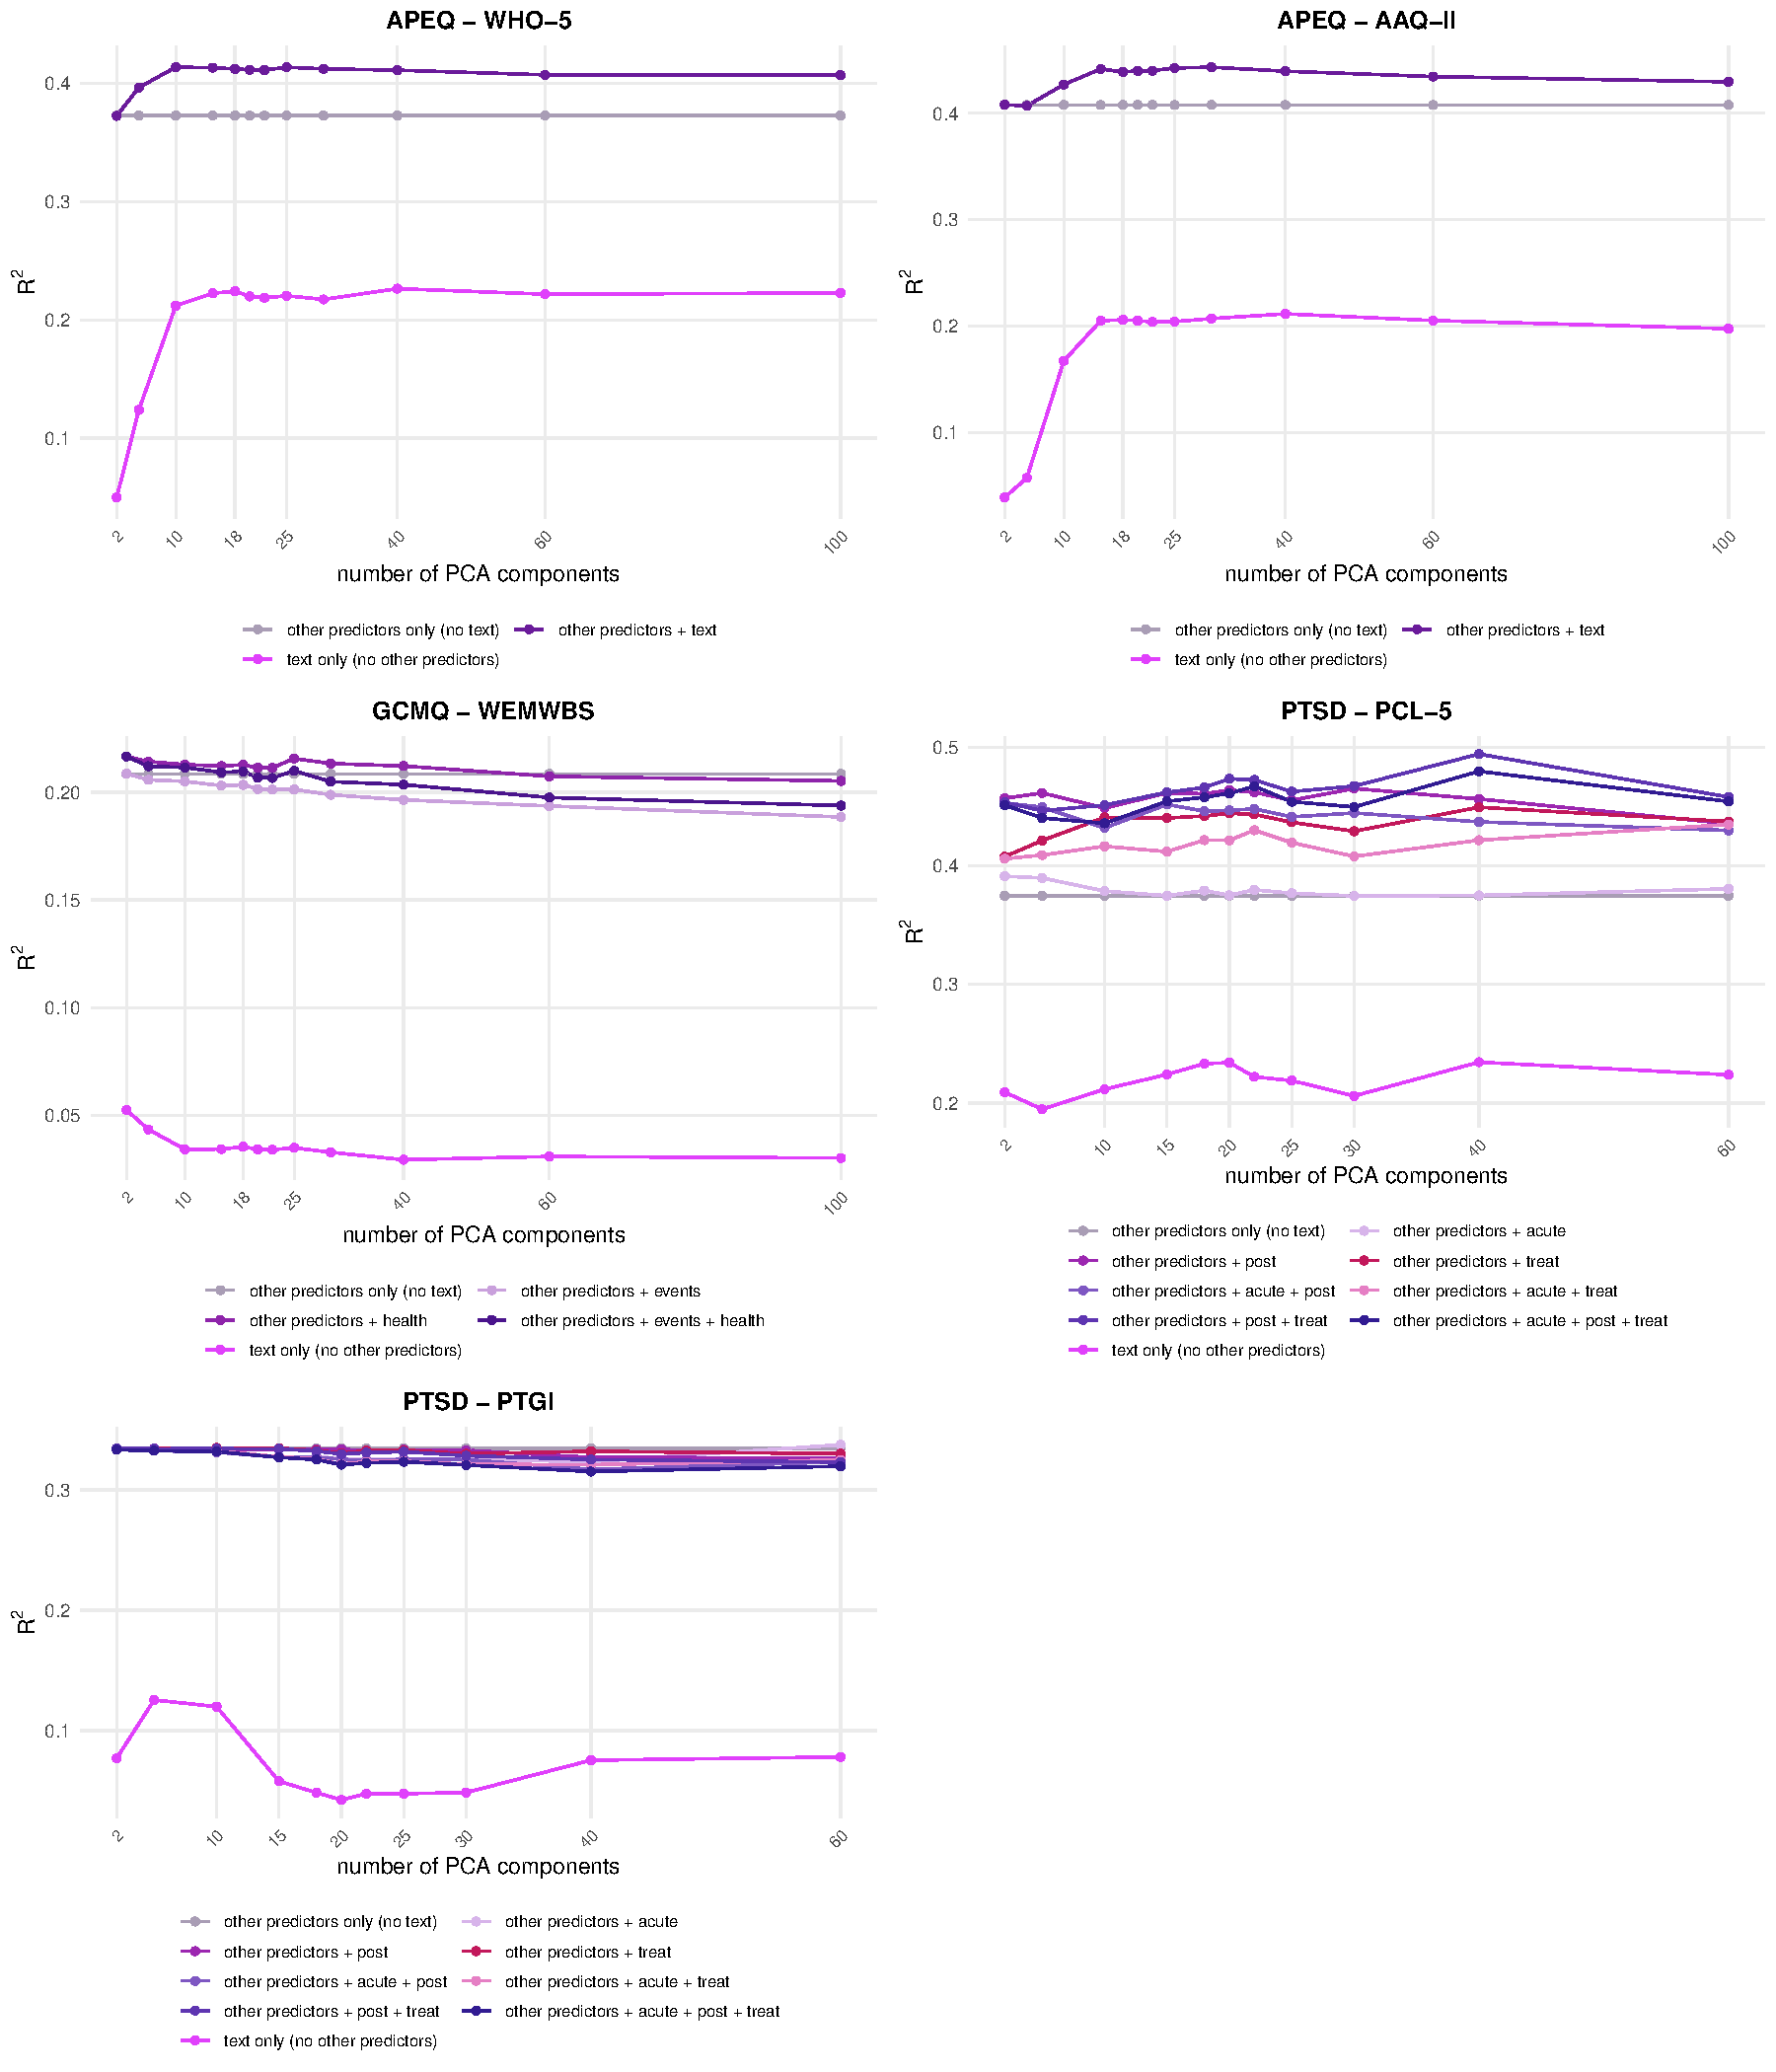
\includegraphics[width=\textwidth]{generated/fig_sweeps_e5.pdf}
  \caption{Cross-validated $R^2$ against the number of retained PCA components, for each dataset and outcome\change{ (single \res{set.folds}-fold cross-validation run)}. Text embeddings: multilingual-e5-large.}
  \label{fig:sweeps-e5}
\end{figure}

\newpage

\begin{figure}[ht!]
  \centering
  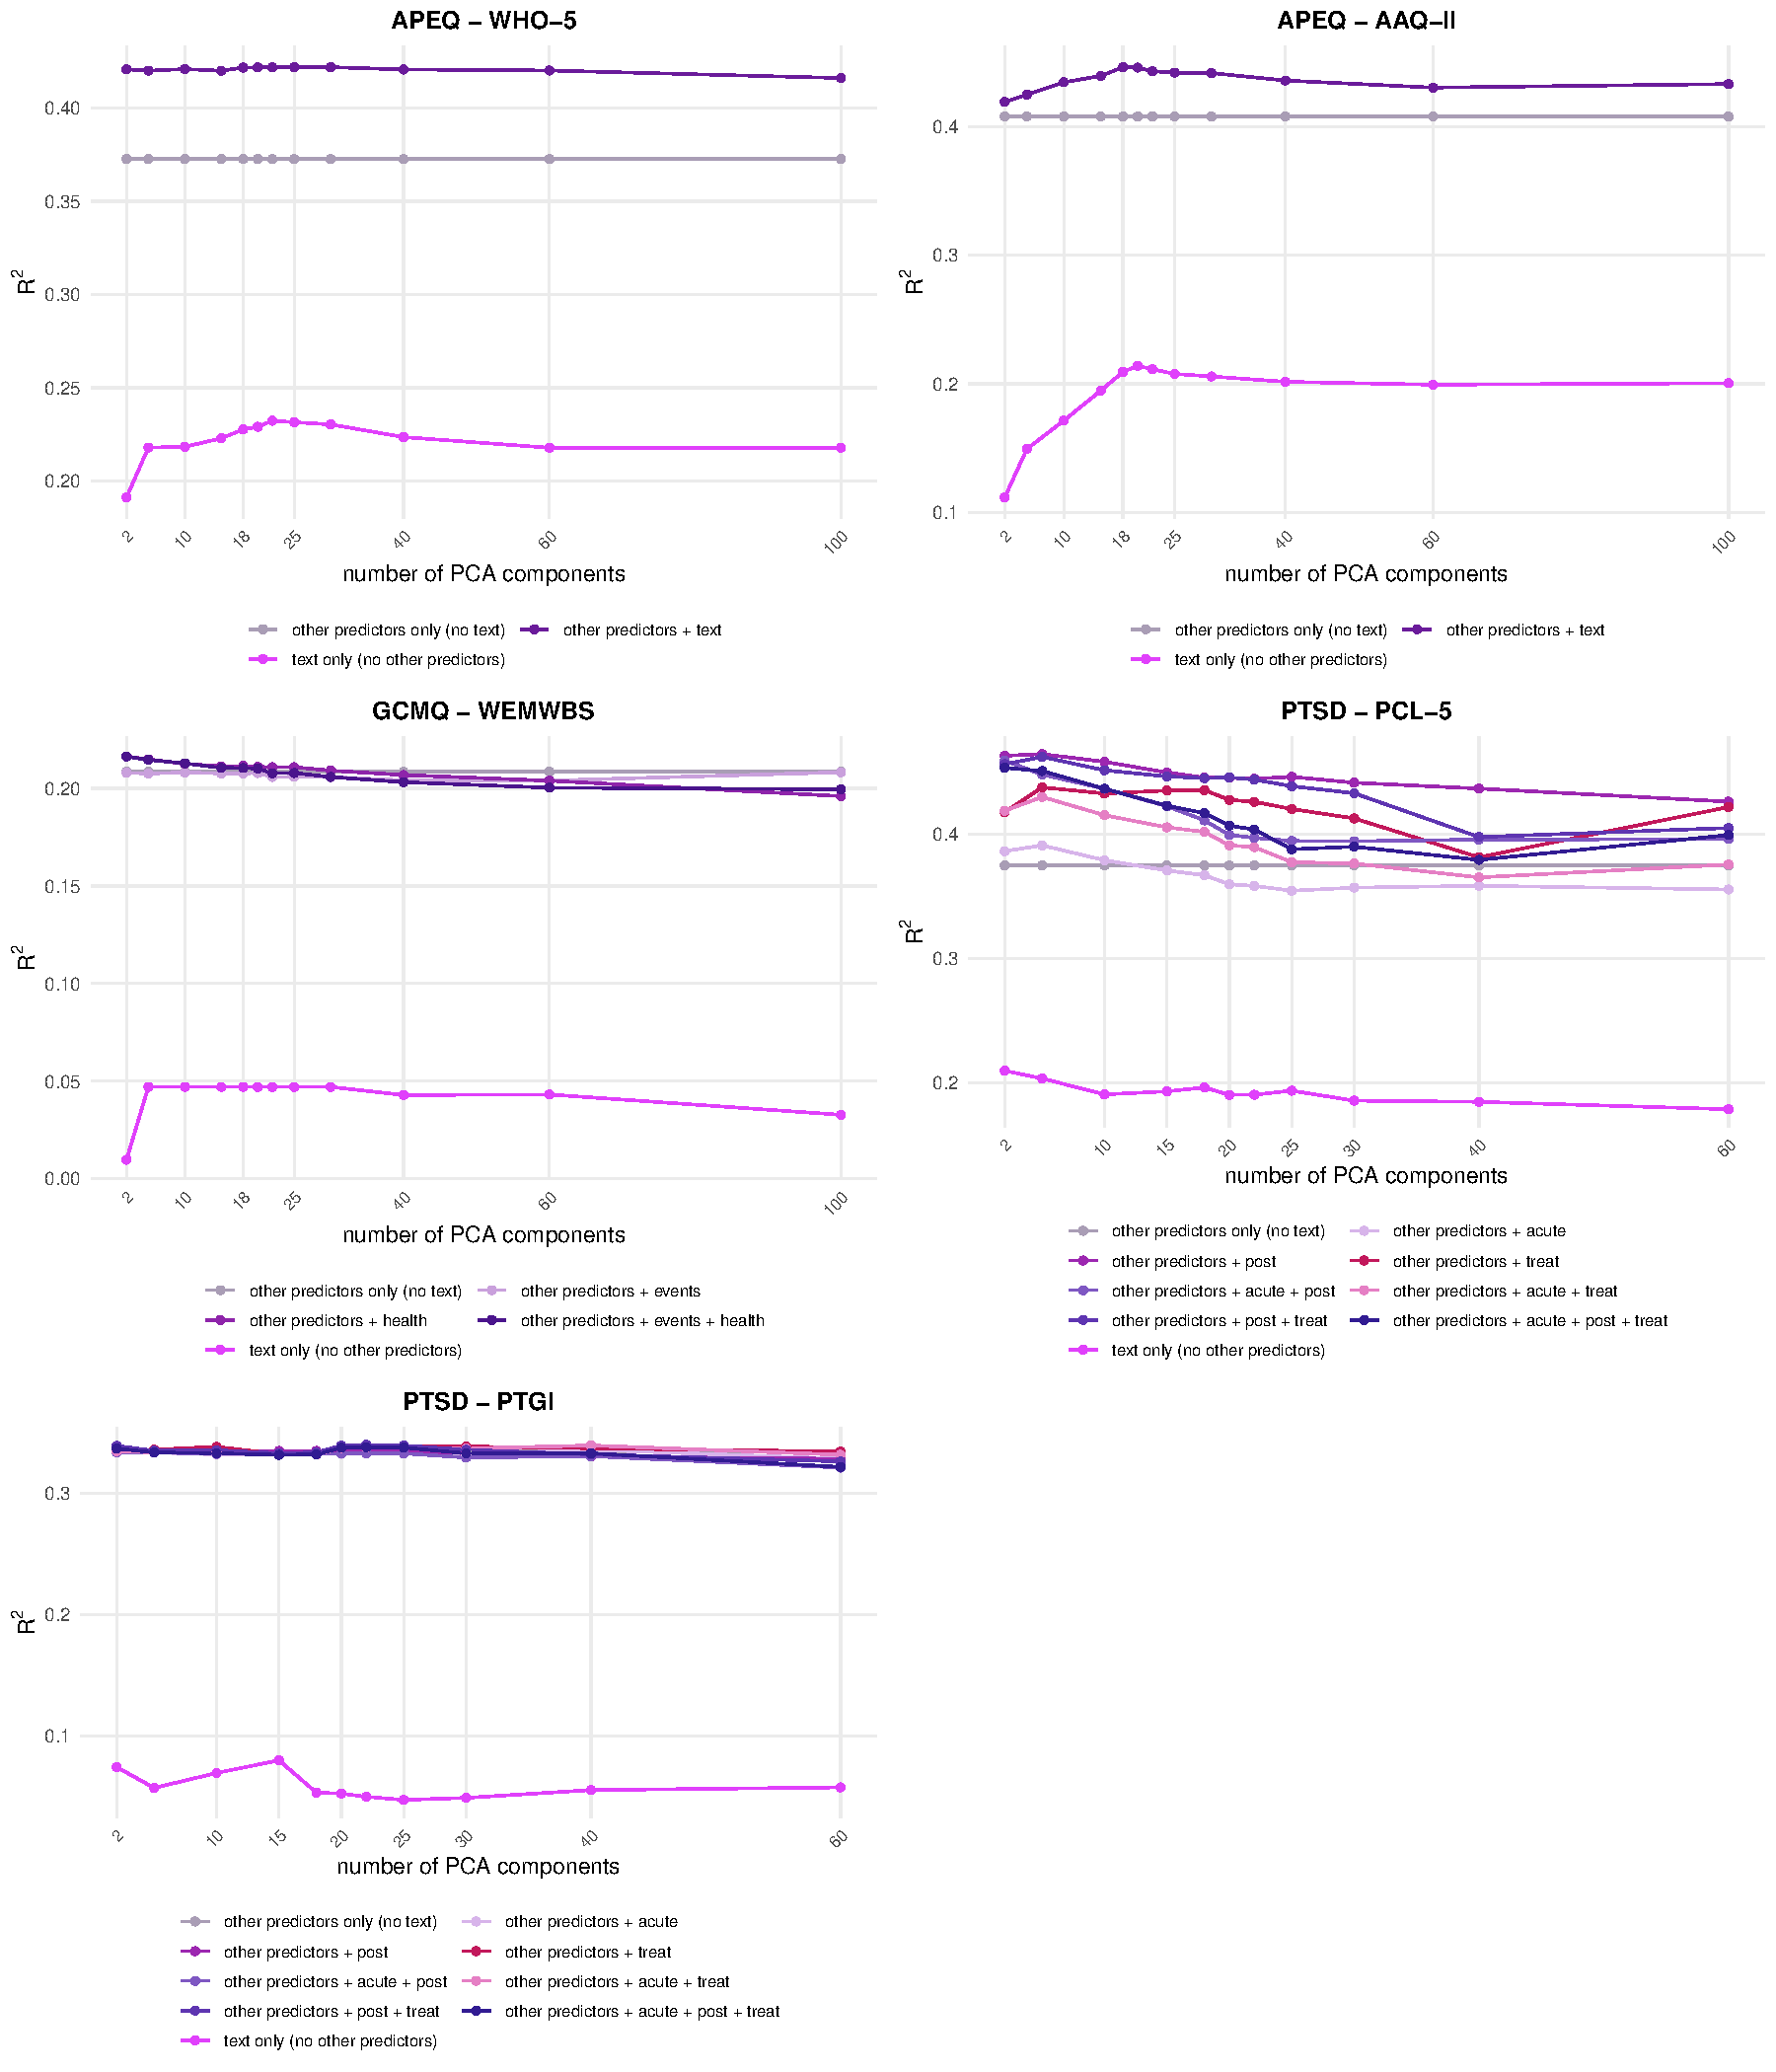
\includegraphics[width=\textwidth]{generated/fig_sweeps_bge.pdf}
  \caption{Cross-validated $R^2$ against the number of retained PCA components, for each dataset and outcome\change{ (single \res{set.folds}-fold cross-validation run)}. Text embeddings: bge-m3.}
  \label{fig:sweeps-bge}
\end{figure}
    
\end{document}
